\documentclass{yorkThesis}

%%%%%%%%%%%%%%%%%%%%%%%%%%%%%%%%%%%%%%%%%%%%%%%%%%%%%%%%%

\usepackage[utf8]{inputenc}

%%%%%%%%%%%%%%%%%%%%%%%%%%%%%%%%%%%%%%%%%%%%%%%%%%%%%%%%%

\newcommand{\lorem}{Lorem ipsum dolor sit amet, consectetur adipiscing elit, sed do eiusmod tempor incididunt ut labore et dolore magna aliqua. Ut enim ad minim veniam, quis nostrud exercitation ullamco laboris nisi ut aliquip ex ea commodo consequat. Duis aute irure dolor in reprehenderit in voluptate velit esse cillum dolore eu fugiat nulla pariatur. Excepteur sint occaecat cupidatat non proident, sunt in culpa qui officia deserunt mollit anim id est laborum.\\}

%%%%%%%%%%%%%%%%%%%%%%%%%%%%%%%%%%%%%%%%%%%%%%%%%%%%%%%%%

\title{
{Approximating Motivation-Related Latent States in \\ Large Scale Scenarios}\\
{\small Applications to Engagement Prediction in a Videogames Setting.}\\

{\large University of York}
}
\author{Valerio Bonometti}

%%%%%%%%%%%%%%%%%%%%%%%%%%%%%%%%%%%%%%%%%%%%%%%%%%%%%%%%%

\begin{document}

\maketitle

\chapter*{Abstract}
\lorem

\chapter*{Dedication}
\lorem

\chapter*{Declaration}
The work presented in this thesis was developed as a partnership between University of York and Square Enix Ltd. It was supported by the EPSRC Centre for Doctoral Training in Intelligent Games \& Games Intelligence (IGGI) grant number [EP/L015846/1]. All data employed in this work were obtained and processed in compliance with the European Union's General Data Protection Regulation \cite{EUdataregulations2018} and Square Enix Ltd. data protection policies. Chapter \ref{chapter_theory_modelling} is based on the work carried out in \cite{bonometti2020theory, bonometti2021approximating}. Chapter \ref{chapter_implementation_testing} is based on the work carried out in \cite{bonometti2019modelling, bonometti2020theory, bonometti2021approximating}. Chapter \ref{chapter_repr_anal} is based on the work carried out in \cite{bonometti2021approximating}.

\chapter*{Acknowledgements}
\lorem

\tableofcontents

%%%%%%%%%%%%%%%%%%%%%%%%%%%%%%%%%%%%%%%%%%%%%%%%%%%%%%%%%

\chapter{Introduction}
\label{chapter_intro}
\section{General Introduction}
When we see a professional athlete competing at an event we often find ourself thinking "how much work they must have done to reach such level of performance". Similarly we might be surprised discovering the effort miners were putting in finding even small ammount of gold nuggets during the \nth{19} century gold rush, and we widen our eyes looking at how many hours we sank watching the latest Netflix series or playing our favourite videogames. But what do all these activities have in common? They are very different from each other but nevertheless able to elicit prolonged and vigorous behavioural responses. Indeed, it appears that human being are capable of remarkable feats when trying to achieve goals that lead to positive and pleasurable outcomes for them. From psychological point of view, we say that in all those instances a common set of cognitive and affective processes, which go under the umbrella of "Motivation", are involved in the generation of goal-directed behaviour. This implies that knowing the motivational state of an individual, during a particular activity, puts us in a favourable position for interpreting their behaviour and predicting its future intensity. Within this general framework lies the aim of this thesis. With the current work we attempted to develop a methodology for approximating the motivational states of individuals in situations where large volumes of observational data are present but a direct contact with the individuals is not possible.


\section{Thesis Outline}
The goal of this thesis is to design, develop and test a methodology for approximating the motivational states of individuals in situations where large volumes of observational data are present but it is not possible to have direct contact with the individuals that generated them. Chapter one with a general outline on motivation and reward-driven motivation in particular. Stemming from here it highlights, how from a behavioural point of view, engagement can be seen as a derivative of the motivational state in which an individual is. Next, It continues showing how motivation can be conventionally assessed highlighting strengths and weaknesses of different approaches with particular attention to applications in large scale scenarios. The chapter closes on a review of works for estimating motivation and engagement at large scale with a particular focus on applications in a video game context. Chapter two aims to illustrate how we can leverage knowledge from theories of motivation for designing data driven solution for the estimation of the motivational state of individuals and engagement prediction. It opens with the illustration of a computational model of incentive salience, a particular theoretical account of reward-driven motivation, and it continues showing how the principles of this model can be used for defining the architecture of an artificial neural network. The chapter closes with a series of experiments aiming to assses the profiiency of the derived model through model comparison. Chapter three aims to illustrate how it is possible to extract and inspect the representantion generated by an articial neural network. It opens illustrating the concept of representation learning in the context of artificial neural network and it proceeds illustrating a series of methodologies for analyzing this representations and deriving insights from it. Chapter four illustartes how the model designed in chapter 2 can be extended and improved. Chapter 5 shows a potential application of the work carried out in this thesis for large scale engagement estimation in a videogame context.




\chapter{Literature Review}
\label{chapter_lit_review}
\section{Introduction}
\label{motivation_engagement_introduction}

\section{Motivation as a Reward-Driven Process}
\label{motivation}

The construct of motivation is a key concept for understanding why individuals seek out specific objects or experiences at particular times and why they react in particular ways when encountering stimuli considered of particular relevance [1]. In this view motivation can be defined as the process leading the modulation and reiteration of goal directed behaviours that once reached exerts rewarding (i.e. pleasurable) effects on the individual [2]. What is a common confound when defining this phenomenon is to partition it in different sub-components each one supposedly representing a different version of the motivational process (e.g. the motivation of X, the X motivation) [3]. The motivational process remains always the same, what changes is the nature of the goal producing the motivated behaviour [2]. If we represent motivation as a vector, its length would be the intensity of pursuit (or the amount of goal directed behaviour) while the angle the focus on a specific goal [2]. Summarizing we can say that the behaviour of an individual is motivated by the expectancy of pleasurable outcomes derived by the goal the behaviour is aiming to reach [1]. The aforementioned statement becomes particularly relevant for those spontaneous activities which are not driven by the fulfilment of fundamental needs (e.g. hunger or thirst) or by the avoidance of negative consequences (e.g. cognitive or physical pain), indeed for these activities what matters is the nature of the goal which may largely vary among individuals. Having a clear definition of the motivational process in place will help us understanding how some of the findings regarding motivational factors in videogames can be reframed in a behavioural context.

\subsection{An Historical View on Reward-driven Motivation}
\label{motivation_hist}
One of the early theorizations of human motivation proposed that individuals were motivated by the expectance of incentive outcomes. These expectations are formed through a process in which an individual learn the existence of an association between the actions he performs and the potential pleasurable outcomes associated to them [1]. Extending on this conceptualization, it has been proposed that the learning process does not only provide a way for forming the expectation of a pleasurable outcome in response to a specific behaviour but also allow to perceive the behaviour itself as source of hedonic reward [1], this concept of hedonic reward will be clarified later in this section as it constitutes an interesting point of connection with existing models of motivational factors in videogames. A third theoretical formulation, which fuses the two aforementioned approaches, making use of  concept related to learning through reinforcement formulated that a stimulus and the behaviours associated to it become relevant and salient for an individual as a consequence of learning its rewarding properties [1]. What written in this paragraph seems very distant from our initial starting point, to a certain extent an over-simplistic lab rat view on human behaviour, but what has been described here is one of the fundamental and most elegant (in terms of complexity to explanatory power ratio) mechanism able to explain and describe at why people do what they do, why they keep doing it and why they do that for a specific amount of time. Obviously taking this as the ultimate explanatory approach would be not just naïve but wrong as many layers of complexity need to be applied for approaching a good description of the motivational process in humans, however we can see some similarities with our previous overview on engagement: the relationships between the individual and the activity preformed, the ability of the activity in providing pleasurable experience and the necessity of feedback (i.e. reward) for maintaining engagement.

\subsection{Learning mechanisms: classical and operant conditioning}
\label{classical_operant_cond}
We will now illustrate the concepts of classical and operant conditioning, basic learning processes which are fundamental for introducing the higher level concept of incentive salience later on. For understanding the processes of classical and operant conditioning it is worth defining what a reinforcing object and process are. We can describe as reinforces those object having the capability to alter the probability of appearance of a specific behaviour [34, 35, 36].  On the other hand the reinforcing process identify the development of a condition in which a specific behaviour becomes more probable when followed by particular reinforcing events and becomes less probable when this last ones are not present anymore [34]. Reframing this concepts in a videogame context we can hypothesize that in-game contents or mechanics act as reinforcing objects when they produce positive outcomes for the player, in a cyclic process in which interacting with the game might produce positive reactions player-activity interactions which in response will make new interactions with the game more probable. 
We will now see the how classical and operant conditioning operationalize the aforementioned concepts of reinforcing object and process.
CLASSICAL CONDITIONING
Classical conditioning describes a learning process in which, independently from the activity of an individual, the repeated pairing of two stimuli will cause one to acquire the eliciting properties of the other [36]. Employing the aforementioned concepts of reinforce, the repeated pairing of a neutral object with reinforcing consequences will imbue the first with reinforcement properties. This concept is extremely simplistic and not suitable for describing human behaviour, however succinctly illustrate a very basic and common learning process other than being the ground from which operant conditioning stems.
OPERANT CONDITIONING
Operant conditioning extends on the concept of classical condition introducing the agency of the individual. The concept refers to the process in which the frequency of a behaviour tends to increase when precise consequences are associated to it [35]. In this view, an operant is formalized as a goal directed behaviour while all the elements reinforcing the re-iteration of this behaviour are called reinforces [35]. The learning process here results from the relationship between a behaviour and its consequences, therefore the probability of behaviour to take place is related to its capability to produce reinforcement [34]. Again, reframing this concept in a videogame context the goal directed behaviour would be the interaction with the game environment while the reinforces are the consequences generate by the interaction itself, which might come in form of internal state only (i.e. pleasurable experiences) or also in the form of in game rewards (i.e. game feedbacks). 

\subsection{Reward and Incentive Salience Attribution}
\label{incentive_salience}
Until now we have mainly used the terms reinforces and incentives for identifying stimuli able to drive and shape behaviour, but when it comes to define effective reinforces, is not just a matter of merely pairing a behaviour with a stimulus but the stimulus itself has to have particular properties. In this view, stimuli able to generate pleasurable feelings in the individual are the best candidates for being effective reinforces,  they are said having ‘rewarding properties’.  But what is, and how can be defined the reward?  The reward is a process generated in response to a stimulus making it desirable for its capacity to generate pleasurable responses. In this view, for being able to generate rewarding response, a stimulus needs two fundamental properties: it has to be wanted (i.e. it acquires the capacity to become desirable) and liked (i.e. it has to be able to generate pleasure in the individual) [37]. But how a particular object acquires this properties? Here comes in action the aforementioned learning processes: the repeated pairing between a stimulus and the reaction it generates in the individual imbue the first with rewarding properties. Moreover, through the aforementioned learning process (i.e. operant conditioning) not just the stimulus itself but also the connected instrumental behaviour will likely acquire the same rewarding properties [37]. A useful distinction that can be me here is between stimuli having primary and secondary reward properties:
Primary rewards 
These are type of stimuli having intrinsic rewarding properties due to their linkage with essential evolutionary needs (i.e. satisfaction of homeostatic needs),  the rewarding properties don’t have to be learned but already present, up to a certain extent, in the stimulus itself [45]. 
Secondary rewards
these are type of stimuli which don’t hold an innate capacity to generate rewarding experiences, their capacity to generate pleasurable experiences and consequently being wanted is strongly related to the occurrence of some of the aforementioned learning processes [45].

Despite this distinction might seems superfluous at a first glance, it has a particular relevance for understating the framework in which videogames lies. No element in a videogame context possesses intrinsic rewarding properties, here the learning process is essential for allowing the element to acquire the aforementioned rewarding properties. The attractive property of an in-game element is not present before the user start playing the game but it might be learned through the user – game interactions occurring during the playing activity.

\paragraph{Wanting}
\label{wanting}
\lorem

\paragraph{Liking}
\label{liking}
\lorem


\paragraph{Learning}
\label{learning}
Classical conditioning describes a learning process in which, independently from the activity of an individual, the repeated pairing of two stimuli will cause one to acquire the eliciting properties of the other [36]. Employing the aforementioned concepts of reinforce, the repeated pairing of a neutral object with reinforcing consequences will imbue the first with reinforcement properties. This concept is extremely simplistic and not suitable for describing human behaviour, however succinctly illustrate a very basic and common learning process other than being the ground from which operant conditioning stems.

Operant conditioning extends on the concept of classical condition introducing the agency of the individual. The concept refers to the process in which the frequency of a behaviour tends to increase when precise consequences are associated to it [35]. In this view, an operant is formalized as a goal directed behaviour while all the elements reinforcing the re-iteration of this behaviour are called reinforces [35]. The learning process here results from the relationship between a behaviour and its consequences, therefore the probability of behaviour to take place is related to its capability to produce reinforcement [34]. Again, reframing this concept in a videogame context the goal directed behaviour would be the interaction with the game environment while the reinforces are the consequences generate by the interaction itself, which might come in form of internal state only (i.e. pleasurable experiences) or also in the form of in game rewards (i.e. game feedbacks).

We will now illustrate the concepts of classical and operant conditioning, basic learning processes which are fundamental for introducing the higher level concept of incentive salience later on. For understanding the processes of classical and operant conditioning it is worth defining what a reinforcing object and process are. We can describe as reinforces those object having the capability to alter the probability of appearance of a specific behaviour [34, 35, 36].  On the other hand the reinforcing process identify the development of a condition in which a specific behaviour becomes more probable when followed by particular reinforcing events and becomes less probable when this last ones are not present anymore [34]. Reframing this concepts in a videogame context we can hypothesize that in-game contents or mechanics act as reinforcing objects when they produce positive outcomes for the player, in a cyclic process in which interacting with the game might produce positive reactions player-activity interactions which in response will make new interactions with the game more probable. 
We will now see the how classical and operant conditioning operationalize the aforementioned concepts of reinforcing object and process.

\section{What is Engagement: A Behavioural Perspective}
\label{engagement}
Playing games has always been present in human history as an occupation aiming to entertain and relax [42], it can be defined as a free-time activity with spatial and temporal boundaries able to intensely absorb who is involved in it [42]. A special case of the broader group of games are those being delivered and experienced in a digital format (i.e. videogames) which since various decades has been substituting more traditional ludic activities [42, 43]. This phenomenon has been well reflected both in terms of number of people involved in playing videogames as well as in the amount of time spent engaging in this activity [44]. One of the main reasons for this explosive phenomenon relies on the fact that videogames seems to be perfect medium for delivering enjoyable experiences [32], consequently holding a strong potential to engage and retain users involved in the playing activity. Various attempt has been made to understand engagement in videogames, both at the level of process and factors driving and influencing it [32].

\subsection{Factors Driving Engagement}
\label{factors_engagement}
The literature reports various theoretical approaches  for addressing the possible different mechanism producing engagement [32], we will briefly illustrates some of the most prominent ones focusing in a second moment on a specific framework connecting engagement to the motivational factors provided by videogames. Focusing on the motivational factors driving engagement is a well suited ground for building a methodology aiming to assess and evaluate engagement via behavioural measures, this because we can take advantage of existing theories describing human behaviour via the interaction between the individual (i.e. the player) and the stimuli (i.e. the game features) present in the environment (i.e. the game world).

Flow
A classical construct employed in the videogame literature for explaining the phenomenon of engagement, is the concept of flow developed by [33]. The formulation of this construct prescribe that when an individual is absorbed in an activity perceived as valuable they will experience a rewarding state of optimal pleasure constituting the fuel for of  engagement process [32]. In this view the conditio sine qua non for the flow state to arise is a balanced combination of the individual’ skill level and the difficulty of the task in which they are involved. Despite offering an interesting point of view, the concept of flow as a framework for explaining engagement in digital games might be prone to the fallacy of circular reasoning: is a user engaged in a specific activity because this provides the optimal flow experience or this last one is a bi-product of being engaged in the activity itself? 

Immersion
A construct linked to the concept of flow is immersion, which differently from flow is concerned with the specific, psychological experience of engaging with a computer game [46]. Immersion is referred as the experience of engaging in one moment in time with a videogame rather than being a factor driving engagement itself [46]. The experience of immersion involves loosing track of time, space and having a sense of being in the task environment, all of this occurring as a result of a good gaming experience. What emerges from the brief overview of the concept of immersion is that rather than posing itself as a factor influencing or driving engagement it seems to provide an alternative approach for describing and characterizing it.

Uses and gratifications
Uses and gratification theory states that users possess different motives characterizing their gratification-seeking behaviours and that these can be satisfied through media consumption [47]. Engagement in this type of activities (i.e. media consumption) is justified by their ability to meet the motives driving the user behaviour. Another point that this theoretical approach assumes is that media audience are not passive but rather variably active, concept that is particularly relevant when evaluating the interaction between players and videogames, since the first have an active role in determining how the latter changes over time[47]. Despite its relatively vague formulation, uses and gratification theory introduce two important concepts: first that users engage in a spontaneous activity (i.e. media interaction) in search of some form of gratification and second that this interaction is not passive but an active process in which the user interact with the medium.

\subsection{The Engagement Process Model}
\label{eng_proc_model}
Various attempts have been made for formalizing the concept of ‘engagement in digital games’, but this appears to be a non-trivial task with the resulting theoretical framework being heterogeneous and not unified [32]. We will employ the work of [40] for providing a general overview on engagement. In [40] engagement is defined as:
‘…a quality of user experiences with technology that is characterized by challenge, aesthetic and sensory appeal, feedback, novelty, interactivity, perceived control and time, awareness, motivation, interest and affect’.
Building on this, [40] avoids to provide an exact definition of engagement but rather describes it as a process with distinct phases each one possessing peculiar attributes.
Point of engagement
It Is the starting point of the engagement process, it configures as the moment in which the user’s attention is directed towards a specific activity due to properties of the activity itself or for its capacity to fulfil specific motivational drives that the user might have.
Period of engagement
It is the period during which the user is having a sustained involvement into the activity and it is fostered by the ability of the activity to provide appropriated feedbacks, novel information and features.
Disengagement
It is defined as the moment in which the users makes an internal decision to stop the activity or when external factors force them to not engage in it anymore. The internal factors are usually connected to loss of interest or pressure derived by the time passing, external factors instead relate to the inability of the activity to provide novelty or to the occurrence of distractors during the activity.
Reengagement
It identifies the moment in which the user returns to the activity after disengagement occurred. This can happen both at short term and long term and it is the result of positive past experiences with the activity, which are usually linked to be exposed to rewarding incentives or novel content within the activity.
What emerges from the description of engagement as process seems to be that a mix of properties of the activity, internal states of the user and ‘environmental’ factors external to the activity itself controls the engagement’s quality and quantity. This consideration will be functional for the theoretical framework we are trying to build through this review.

SUMMARY
The aim of this brief review was not to define or once-for-all clarifying the concept of engagement in digital games (it would be almost impossible other than out of scope) but rather to identify a possible fil rouge connecting the existing works. What emerged seems to point in the direction of engagement being a second order factor emerging from (or generated by) a series of subjective experiences linked to the interaction between the user and the playing activity. What seems to connect all these different approaches seems to be the description of a process in which the interaction between the user and the game activity generates feelings of enjoyment and pleasure ultimately contributing to the engagement in the activity itself [32]. This interpretation will become particularly useful when we will address the concept of reward and incentive salience later on.

\section{Engagement as a Derivative of Motivational Processes}
Motivation and engagement seems to be interchangeable terms but we argue that they are qualitatively different. Motivation pertain the state of an individual with resect to achieving a particular goal, perfroming a particular action or interacting with a particular object. Engagement on the other hand describes the quantity and quality of the interaction both from a behavioural and experiential point of view. From now on the relationship between motivation and engagement will be assumed we will have to rember that engagement, from a behavioural point of view, is a derivative product of the motivational state in which an individual is. 

\section{Measuring Motivation and Engagement}
\label{measuring_motivation_engagement}
\lorem
    \subsection{Self-report Measures}
    \label{self_report}
    \lorem
    \subsection{Psychophisiological Measures}
    \label{psychophisio}
    \lorem
    \subsection{Behavioural Measures}
    \label{behavioural_indices}
    \lorem
    \subsection{Challenges from Large Scale Observational Data}
    \label{challenges_large_scale}
    \lorem

\section{Estimating Motivation and Predicting Engagement from Observational Data}
\label{estpred_motivation_engagement}
\lorem
    \subsection{Latent States Estimation Models}
    \label{latent_estimation}
    \lorem
    \subsection{Engagement Prediction Models}
    \label{engagement_prediction}
    \lorem
    \subsection{Common Features}
    \label{estimation_prediction}
    \lorem

\lorem





\chapter{From Theory to Modelling}
\label{chapter_theory_modelling}
\section{Manifold Representation of Motivation}
\label{neural_manifold}
\lorem
\section{Computational Framework}
\label{comp_framework}
In this chapter, we will propose a way to approximate the manifold structure of attributed incentive salience in scenarios where only large volumes of behavioural data are available and no strict experimental control is possible. First, we will briefly illustrate how previous work has framed the modelling of this construct as a reinforcement learning problem and solved it using Temporal Difference Learning (TD Learning) \cite{sutton1988learning}. This, will provide us with a psycho-biologically plausible computational model of attribute incentive salience and constitute the starting point for our approach. Then, we will highlight how video games are promising candidates for studying the behavioural aspects of incentive salience attribution in naturalistic settings. Finally, combining these two ideas, we will show how estimating the manifold structure of attributed incentive salience can be cast as the solution to a supervised learning problem and why Artificial Neural Networks (ANNs), thanks to their representation learning capabilities, are well suited for the task.

\subsection{Temporal Difference Learning}
\label{td_learning}

The first attempt to model incentive salience attribution was carried out by McClure \textit{et. al.} using TD Learning \cite{mcclure2003computational}. The use of TD Learning in simulation studies involving reward learning, is often motivated by its good approximation of the reward-prediction error signal generated by dopaminergic neurons \cite{schultz1997neural,flagel2011selective}. Algorithms in the family of TD Learning attempt to learn a value function $V$ by iteratively refining an estimate $\widehat{V}$ over time \cite{sutton2018reinforcement}. In the most basic form, called TD(0), this is done by simply observing the reward $r$ associated with a particular state $s$ at time $t_{+1}$ and using it to adjust the estimate of $V$ produced at time $t$ \cite{sutton2018reinforcement}. Here $t$ is an arbitrary unit of time, it can be specific (i.e. seconds) or generic (i.e. a point in an ordered series of events) depending on the type of application. If we let $S=\{s_{t}: t \in T\}$ be a sequence of states, then the value $V$  at $s_{t}$ is given by the sum of all future discounted rewards expected when transitioning from $s_t$ to $s_{t+1}$
\begin{align}
\label{td_v}
    V(s_t) 
        &= E[
            r_{t+1} + 
            \gamma r_{t+2} + 
            \gamma^{2} r_{t+3} +
            ... +
            \gamma^{T} r_{T}
        ]\\
        &= E[
            r_{t+1} + 
            \gamma V(s_{t+1}) 
        ] \nonumber
\end{align}
with $\gamma \in [0, 1]$ being a discounting factor for $r$. The iterative refining of $\widehat{V}$ carried out by TD learning is achieved by first computing an error signal $\delta$ at time $t$
\begin{align}
    \label{td_error}
    \delta(t) = r_{t+1} + \gamma \widehat{V}(s_{t+1}) - \widehat{V}(s_{t})
\end{align}
which quantifies the difference between the current $\widehat{V}$ and what is expected when transitioning to $s_{t+1}$. Once the error signal is computed, $\widehat{V}(s_{t})$ is updated as: 
\begin{align}
    \label{td_update}
    \widehat{V}(s_t)  \leftarrow \widehat{V}(s_t) + \alpha(\delta)
\end{align}
where $\alpha \in [0, 1]$ is a constant controlling the amount of updating or the "learning rate". This process called TD update is illustrated by the diagram presented in Figure \ref{fig: td_learning}. Conventionally the transition from $s$ to $s_{t+1}$ is the result of an action selection process guided by $\widehat{V}$, because in optimal control settings the role of reinforcement learning is to select the course of action that maximizes future rewards \cite{schultz1997neural,mcclure2003computational,sutton2018reinforcement}.
\begin{figure}[h]
  \begin{center}
    \begin{adjustbox}{width=0.7\columnwidth}

        \tikzset{every picture/.style={line width=0.75pt}}       
        
        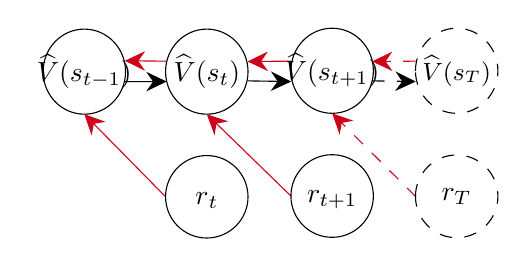
\begin{tikzpicture}[x=0.75pt,y=0.75pt,yscale=-1,xscale=1]
        
        %Straight Lines [id:da2592063600931961] 
        \draw [color={rgb, 255:red, 208; green, 2; blue, 27 }  ,draw opacity=1 ]   (282.5,135.16) -- (300.67,135.02) ;
        \draw [shift={(279.5,135.18)}, rotate = 359.55] [fill={rgb, 255:red, 208; green, 2; blue, 27 }  ,fill opacity=1 ][line width=0.08]  [draw opacity=0] (9.82,-4.72) -- (0,0) -- (9.82,4.72) -- (6.52,0) -- cycle    ;
        %Straight Lines [id:da41585806917853485] 
        \draw [color={rgb, 255:red, 208; green, 2; blue, 27 }  ,draw opacity=1 ]   (223.33,134.87) -- (240.67,135.02) ;
        \draw [shift={(220.33,134.85)}, rotate = 0.47] [fill={rgb, 255:red, 208; green, 2; blue, 27 }  ,fill opacity=1 ][line width=0.08]  [draw opacity=0] (9.82,-4.72) -- (0,0) -- (9.82,4.72) -- (6.52,0) -- cycle    ;
        %Shape: Ellipse [id:dp31493856088290983] 
        \draw   (181,140.07) .. controls (181,128.75) and (189.89,119.58) .. (200.86,119.58) .. controls (211.83,119.58) and (220.72,128.75) .. (220.72,140.07) .. controls (220.72,151.4) and (211.83,160.57) .. (200.86,160.57) .. controls (189.89,160.57) and (181,151.4) .. (181,140.07) -- cycle ;
        %Shape: Ellipse [id:dp5103941395609547] 
        \draw  [dash pattern={on 4.5pt off 4.5pt}] (360.4,139.66) .. controls (360.4,128.34) and (369.29,119.16) .. (380.26,119.16) .. controls (391.23,119.16) and (400.12,128.34) .. (400.12,139.66) .. controls (400.12,150.98) and (391.23,160.16) .. (380.26,160.16) .. controls (369.29,160.16) and (360.4,150.98) .. (360.4,139.66) -- cycle ;
        %Straight Lines [id:da30559831832260953] 
        \draw [color={rgb, 255:red, 0; green, 0; blue, 0 }  ,draw opacity=1 ]   (220.07,144.9) -- (237.5,144.86) ;
        \draw [shift={(240.5,144.85)}, rotate = 539.86] [fill={rgb, 255:red, 0; green, 0; blue, 0 }  ,fill opacity=1 ][line width=0.08]  [draw opacity=0] (9.82,-4.72) -- (0,0) -- (9.82,4.72) -- (6.52,0) -- cycle    ;
        %Shape: Ellipse [id:dp12377292733336898] 
        \draw  [color={rgb, 255:red, 0; green, 0; blue, 0 }  ,draw opacity=1 ] (240,140.07) .. controls (240,128.75) and (248.89,119.58) .. (259.86,119.58) .. controls (270.83,119.58) and (279.72,128.75) .. (279.72,140.07) .. controls (279.72,151.4) and (270.83,160.57) .. (259.86,160.57) .. controls (248.89,160.57) and (240,151.4) .. (240,140.07) -- cycle ;
        %Shape: Ellipse [id:dp9248757796917767] 
        \draw   (300.4,139.66) .. controls (300.4,128.34) and (309.29,119.16) .. (320.26,119.16) .. controls (331.23,119.16) and (340.12,128.34) .. (340.12,139.66) .. controls (340.12,150.98) and (331.23,160.16) .. (320.26,160.16) .. controls (309.29,160.16) and (300.4,150.98) .. (300.4,139.66) -- cycle ;
        %Straight Lines [id:da050274800713848156] 
        \draw [color={rgb, 255:red, 208; green, 2; blue, 27 }  ,draw opacity=1 ]   (202.96,162.71) -- (240,200.37) ;
        \draw [shift={(200.86,160.57)}, rotate = 45.48] [fill={rgb, 255:red, 208; green, 2; blue, 27 }  ,fill opacity=1 ][line width=0.08]  [draw opacity=0] (9.82,-4.72) -- (0,0) -- (9.82,4.72) -- (6.52,0) -- cycle    ;
        %Straight Lines [id:da7059353635730191] 
        \draw [color={rgb, 255:red, 208; green, 2; blue, 27 }  ,draw opacity=1 ]   (262.01,162.66) -- (300.4,200) ;
        \draw [shift={(259.86,160.57)}, rotate = 44.2] [fill={rgb, 255:red, 208; green, 2; blue, 27 }  ,fill opacity=1 ][line width=0.08]  [draw opacity=0] (9.82,-4.72) -- (0,0) -- (9.82,4.72) -- (6.52,0) -- cycle    ;
        %Straight Lines [id:da17885982011746426] 
        \draw [color={rgb, 255:red, 208; green, 2; blue, 27 }  ,draw opacity=1 ] [dash pattern={on 4.5pt off 4.5pt}]  (322.38,162.28) -- (360.4,200.16) ;
        \draw [shift={(320.26,160.16)}, rotate = 44.9] [fill={rgb, 255:red, 208; green, 2; blue, 27 }  ,fill opacity=1 ][line width=0.08]  [draw opacity=0] (9.82,-4.72) -- (0,0) -- (9.82,4.72) -- (6.52,0) -- cycle    ;
        %Shape: Ellipse [id:dp3523005799699832] 
        \draw  [dash pattern={on 4.5pt off 4.5pt}] (360.4,200.16) .. controls (360.4,189.16) and (369.29,180.23) .. (380.26,180.23) .. controls (391.23,180.23) and (400.12,189.16) .. (400.12,200.16) .. controls (400.12,211.17) and (391.23,220.09) .. (380.26,220.09) .. controls (369.29,220.09) and (360.4,211.17) .. (360.4,200.16) -- cycle ;
        %Shape: Ellipse [id:dp3509500153089894] 
        \draw   (300.4,200) .. controls (300.4,189) and (309.29,180.09) .. (320.26,180.09) .. controls (331.23,180.09) and (340.12,189) .. (340.12,200) .. controls (340.12,210.99) and (331.23,219.9) .. (320.26,219.9) .. controls (309.29,219.9) and (300.4,210.99) .. (300.4,200) -- cycle ;
        %Shape: Ellipse [id:dp17336392317383575] 
        \draw  [color={rgb, 255:red, 0; green, 0; blue, 0 }  ,draw opacity=1 ] (240,200.37) .. controls (240,189.4) and (248.89,180.5) .. (259.86,180.5) .. controls (270.83,180.5) and (279.72,189.4) .. (279.72,200.37) .. controls (279.72,211.34) and (270.83,220.23) .. (259.86,220.23) .. controls (248.89,220.23) and (240,211.34) .. (240,200.37) -- cycle ;
        %Straight Lines [id:da21459790152477998] 
        \draw [color={rgb, 255:red, 0; green, 0; blue, 0 }  ,draw opacity=1 ]   (279.5,144.52) -- (297.5,144.8) ;
        \draw [shift={(300.5,144.85)}, rotate = 180.91] [fill={rgb, 255:red, 0; green, 0; blue, 0 }  ,fill opacity=1 ][line width=0.08]  [draw opacity=0] (9.82,-4.72) -- (0,0) -- (9.82,4.72) -- (6.52,0) -- cycle    ;
        %Straight Lines [id:da8588950475203374] 
        \draw [color={rgb, 255:red, 208; green, 2; blue, 27 }  ,draw opacity=1 ] [dash pattern={on 4.5pt off 4.5pt}]  (342.5,135.16) -- (360.67,135.02) ;
        \draw [shift={(339.5,135.18)}, rotate = 359.55] [fill={rgb, 255:red, 208; green, 2; blue, 27 }  ,fill opacity=1 ][line width=0.08]  [draw opacity=0] (9.82,-4.72) -- (0,0) -- (9.82,4.72) -- (6.52,0) -- cycle    ;
        %Straight Lines [id:da9169375689094925] 
        \draw [color={rgb, 255:red, 0; green, 0; blue, 0 }  ,draw opacity=1 ] [dash pattern={on 4.5pt off 4.5pt}]  (339.5,144.52) -- (357.5,144.8) ;
        \draw [shift={(360.5,144.85)}, rotate = 180.91] [fill={rgb, 255:red, 0; green, 0; blue, 0 }  ,fill opacity=1 ][line width=0.08]  [draw opacity=0] (9.82,-4.72) -- (0,0) -- (9.82,4.72) -- (6.52,0) -- cycle    ;
        
        % Text Node
        \draw (320.26,201.59) node    {$r_{t+1}$};
        % Text Node
        \draw (200.86,140.07) node    {$\widehat{V}(s_{t-1})$};
        % Text Node
        \draw (320.26,139.66) node    {$\widehat{V}(s_{t+1})$};
        % Text Node
        \draw (380.26,139.66) node  [font=\small]  {$\widehat{V}(s_{T})$};
        % Text Node
        \draw (259.86,202) node  [color={rgb, 255:red, 208; green, 9; blue, 2 }  ,opacity=1 ]  {$\textcolor[rgb]{0,0,0}{r}\textcolor[rgb]{0,0,0}{_{t}}$};
        % Text Node
        \draw (259.86,140.07) node  [color={rgb, 255:red, 208; green, 9; blue, 2 }  ,opacity=1 ]  {$\textcolor[rgb]{0,0,0}{\widehat{V}}\textcolor[rgb]{0,0,0}{(s_{t})}$};
        % Text Node
        \draw (380.26,200.16) node    {$r_{T}$};

        \end{tikzpicture}
    \end{adjustbox}
  \end{center}
\caption{\textbf{Graphical representation of TD Learning}. Red arrows indicate the flow of the computations for deriving $\delta$ and updating $\widehat{V}$ expressed by equations \ref{td_error} and \ref{td_update}. Black arrows instead indicate the changes of $\widehat{V}$ moving from $s$ to $s_{t+1}$. Solid circles indicate states which have already been observed while dashed ones represent future not-yet observed states.}
\label{fig: td_learning}
\end{figure}
McClure \textit{et. al.} proposed that incentive salience is represented by $V$ as defined in equation \ref{td_v} while the error signal expressed by equation \ref{td_error} represents the activity of dopaminergic neurons with the dual function of driving the attribution of incentive salience (through reward prediction error coding as specified in section \ref{incentive_salience}) and guiding the previously mentioned action selection process \cite{schultz1997neural,mcclure2003computational,o2003temporal}. However, in later work, Zhang \textit{et. al.} highlighted the fact that the model proposed by McClure \textit{et. al.} fails to take into account an important part of the original incentive salience hypothesis: the dynamic modulation produced by the individual's internal state (see section \ref{wanting}) \cite{toates1994comparing,mcclure2003computational,berridge2004motivation,zhang2009neural,tindell2009dynamic,berridge2012prediction}. Zhang \textit{et. al.} therefore proposed a modification of the original TD Learning model to include a modulatory factor $k \in [0, +\infty]$ which can enhance ($k > 1$), dampen or even revert ($k < 1$) previously learned incentive salience values
\begin{align}
    \label{zhang_td_v}
    V(s_t) = E[\tilde{r}(r_{t+1},k_{t}) + \gamma V(s_{t+1})]
\end{align}
here $\tilde{r}(.,.)$ is a function of two variables and can assume either an additive or multiplicative form \footnote{See \cite{zhang2009neural} for detailed description of the two forms and their functional differences.}. The main difference between the approaches of McClure \textit{et. al.} and Zhang \textit{et. al.} lies in the interpretation of $V$. Both authors see it as a combination of cached value (i.e. what has been learned from past experiences) and expectation over future $r$ but for McClure \textit{et. al.} all the future $r$ have the same weight while for Zhang \textit{et. al.} the state of the individual dynamically modulates the weighting of $r$. Using the notation from section \ref{incentive_salience}, we can say that the interaction $s$ between $I$ and $O$ at time $t_{+1}$ arises from the $V$ (i.e. incentive salience) generated after $s_{t}$. The mismatch between the predicted amount of reward and the actual reward received at time $t_{+1}$ generates an error signal that allows $I$ to learn about the "correct" magnitude of $V(s_{t})$ \cite{schultz2017reward} . As an example, an individual may anticipate that eating their favourite meal would be a rewarding experience but instead (for some reason) it was underwhelming. They therefore reduce the salience previously attributed to it. Importantly, $V(s_{t})$ does not just encompass the previous history of interactions between $I$ and $O$ but also the current state of $I$: the individual has learned from long experience that eating is a pleasurable activity but currently, since they are sated they do not expect much reward from doing it again in the near future.  

\paragraph{\textbf{From TD to Supervised Learning}}
\label{td_to_supervised}
The approaches discussed above frame the estimation of attributed incentive salience as a reinforcement learning task. This requires the simulation of a sequence of interactions between $I$ and $O$ and the concomitant delivery of $r$  \cite{schultz1997neural,mcclure2003computational,zhang2009neural}. However, it is not always straightforward to replicate these interactions in real world scenarios, especially when dealing with human participants. The control on the internal state of $I$ and amount of $r$ delivered that McClure and Zhang assume is usually based on strict assumptions and can be achieved only in controlled experimental settings \cite{mcclure2003computational,zhang2009neural}. As an alternative solution for inferring $V$ outside the laboratory we propose to learn its manifold structure through supervised learning. Differently to what reported in the literature \cite{calhoun2019unsupervised, mccullough2021unsupervised, luxem2020identifying, pereira2020quantifying, shi2021learning} we argue that in this case the use of supervised in place of un-supervised techniques is to be preferred. Indeed, since we are dealing exclusively with behavioural data and trying to solve an inverse problem  we would like to learn a manifold structure which is not just a generic indicator of behavioural phenotype \cite{luxem2020identifying} but also obeys to specific functional constrains.\\
\\
In this approach, an experimenter gathers data on a set of interactions between $I$ and $O$ and let a learning algorithm to estimate two functions:
\begin{gather}
\label{supervised_v}
    V(s_{t}) = f^{1}(O, \tilde{r_{t}}, V(s_{t-1}); \theta^{1}) \\
    r_{t+1} = f^{2}(V(s_{t}); \theta^{2}) \nonumber
\end{gather}
here $f^{1}$ and $f^{2}$ are arbitrarily complex functions while $\theta^{1}$ and $\theta^{2}$ are parameters that the learning algorithm has to infer. The future reward that an individual expects after an interaction with an object is produced by the current level of attributed salience, which  itself is a function of the current internal state of the individual (expressed through the amount of reward just experienced) and the incentive salience previously attributed to the object. It is important to note that the two functions above need to be recursive over all $s \in S$ (see equations \ref{td_v} and \ref{zhang_td_v}) in order to provide $V(s_{t})$ with the dual purpose of caching all the past $V$ and being a suitable predictor for all the $r$. This formulation however still requires a measure of the $r$ experienced by $I$ (or more precisely its weighted version $\tilde{r}$) after interacting with $O$, which is not easily accessible. However, Thorndike's law of effect \cite{thorndike1927law} and Skinner's operant conditioning principles \cite{skinner1965science} suggest that $r$, which  like $V$ is a non observable latent variable, manifests itself through the intensity of interactions between $I$ and $O$ (i.e. $B$ in Figure \ref{fig: incs} and section \ref{motivation}): the frequency and amount of object-directed behaviours increase or decrease as a function of the rewards an individual expects to receive \cite{berridge2004motivation,schultz2017reward}. Since $V(s_{t})$ predicts how much $r$ an $I$ expects to receive from interacting with $O$, we should also expect the strength of their future interactions to be a function of $V(s_{t})$. This can be represented re-arranging the equations in \ref{supervised_v} in a more compact form as a chain of functions
\begin{align}
\label{supervised_b}
    B_{t+1} = f^{2}(f^{1}(O, B_{t}, V(s_{t-1}); \theta^{1});  \theta^{2})
\end{align}
To approximate the above expression, a learning algorithm would require records of behaviours generated by individuals while interacting with a diverse set of potentially rewarding objects. Here, we argue that video games are one way to obtain this type of data at scale while also achieving some level of ecological validity.

\subsection{Video Games and Telemetry}
\label{videogame_telemetries}
Interacting with video games is a volitional activity driven largely by the capacity of the games to provide pleasurable experiences \cite{boyle2012engagement}. Behaviour within the game is best understood as the result of a value attribution process similar to that of secondary reward objects (see section \ref{incentive_salience}). Indeed, it appears that the play behaviour is often produced and maintained by the structural characteristics of the game (e.g. game mechanics) \cite{king2010video} which, working like conventional reinforcement mechanisms \cite{chumbley2006affect,wang2011game,phillips2013videogame,avserivskis2017computational}, produce effects similar to operant conditioning \cite{skinner1965science}. Although caution should be applied when complex activities are investigated using neuroimaging techniques, evidence suggest that the maintenance of video games playing behaviour engages the same cortico-striatal structures \cite{hoeft2008gender,mathiak2011reward,cole2012interactivity,klasen2012neural,lorenz2015video,gleich2017functional} and neurotransmitters \cite{koepp1998evidence} involved in reward processing. This, seems also supported at the behavioural level where the ammount of experienced in-game reward appears to play a role in controlling how likely is an individual to keep engaging in playing behaviour \cite{agarwal2017quitting, steyvers2019joint}. This, in conjunction with a growing literature highlighting similarities between certain video game mechanics and activities driven by secondary rewards (e.g. gambling) \cite{king2010role,drummond2018video,zendle2018video}, corroborates the idea that video games are able to elicit behavioural responses through incentive mechanics. In this view, video games with different structural characteristics could be seen as objects possessing rewarding properties that heavily depend on the individuals interacting with them (e.g. an individual's preference for a specific game mechanic). Hence, similarly to the process specified in section \ref{theoretical_framework}, we can expect that through repeated interactions, an individual will experience varying degrees of reward determined by their internal state and the characteristics of the game. These interactions will produce continuous adjustments in the level of saliency attributed to playing that specific game which in turn will influence the frequency and amount of future interactions with that same game. Other than offering a context for observing the process of incentive salience attribution, video games allow us to obtain large volumes of behavioural data (similar to those mentioned in section \ref{td_to_supervised}) in a naturalistic fashion. This is made possible by the widespread practice of obtaining high frequency records (i.e. telemetry\footnote{See \cite{el2016game} for a more technical description of telemetry in video games.}) of players' behaviour during the game \cite{drachen2015behavioral}. This approach, despite offering less control and rigour than conventional experimental procedures, allows us to obtain a more faithful representation of natural behaviour (similarly to field studies) while avoiding some of the limitations connected with laboratory-based studies (e.g. sampling and observer biases).
\newline
\newline
In order to use this type of behavioural data to model attributed incentive salience, a learning algorithm should possess the following properties. First, it should be scalable and noise resilient, to leverage large volumes of naturalistic data in an efficient and effective manner. Second, it should be able to approximate arbitrarily complex functions, given that the shape of the functions specified in equation \ref{td_to_supervised} is not known a-priori. And finally, it should be able to produce an approximation of $V(s_{t})$ that can be inspected in order to evaluate if its functional properties can be compared with those of attributed incentive salience. Artificial Neural Networks (ANNs) appear to satisfy these requirements.

\subsection{Artificial Neural Networks}
\label{artificial_neural_networks}
In their conventional form, ANNs can be seen as chains of nested functions (the layers of the network). These layers are vector valued (there are multiple units or neurons in each layer) and organized as directed acyclic computational graphs (information only flows forward). When the number of layers is greater than two, the prefix "deep" is usually applied \cite{bengio2017deep}. The goal of this ensemble of functions is to create a mapping between an input $x$ and a target $y$. Following the example illustrated in Figure \ref{fig: ffnn}, given the set of parameters $\Theta = \{\theta^1, \theta^2 \}$ an ANN would first infer a function $h = f(x;\theta^{1})$, mapping the input to a new representation $h$. The same representation $h$ would then become the input of a second function $\widehat{y} = f^{1}(h;\theta^{2})$ which produces an estimate of the target \cite{bengio2017deep}. In this sense, we can think of each layer as a collection of many non-linear vector to scalar functions taking the previous layer as input and generating the units for the layer that follows \cite{bengio2017deep}. By increasing the number of layers and units, ANNs can approximate an extremely large class of functions \cite{rumelhart1986learning}.
\begin{figure}[h]
    \begin{center}
        \begin{adjustbox}{width=0.6\columnwidth}
            \tikzset{every picture/.style={line width=0.75pt}} %set default line width to 0.75pt        
            
            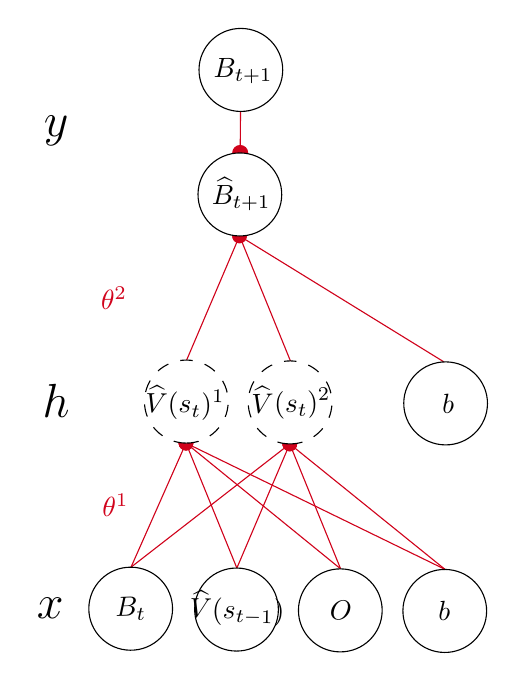
\begin{tikzpicture}[x=0.75pt,y=0.75pt,yscale=-1,xscale=1]
            %uncomment if require: \path (0,350); %set diagram left start at 0, and has height of 350
            
            %Straight Lines [id:da8866607252953388] 
            \draw [color={rgb, 255:red, 208; green, 2; blue, 27 }  ,draw opacity=1 ]   (227.88,279.44) -- (254.36,219.65) ;
            \draw [shift={(254.36,219.65)}, rotate = 293.89] [color={rgb, 255:red, 208; green, 2; blue, 27 }  ,draw opacity=1 ][fill={rgb, 255:red, 208; green, 2; blue, 27 }  ,fill opacity=1 ][line width=0.75]      (0, 0) circle [x radius= 3.02, y radius= 3.02]   ;
            %Straight Lines [id:da0731191645042184] 
            \draw [color={rgb, 255:red, 208; green, 2; blue, 27 }  ,draw opacity=1 ]   (254.68,179.65) -- (280.16,119.85) ;
            \draw [shift={(280.16,119.85)}, rotate = 293.08] [color={rgb, 255:red, 208; green, 2; blue, 27 }  ,draw opacity=1 ][fill={rgb, 255:red, 208; green, 2; blue, 27 }  ,fill opacity=1 ][line width=0.75]      (0, 0) circle [x radius= 3.02, y radius= 3.02]   ;
            %Straight Lines [id:da4826752085294559] 
            \draw [color={rgb, 255:red, 208; green, 2; blue, 27 }  ,draw opacity=1 ]   (304.68,180.05) -- (280.16,119.85) ;
            \draw [shift={(280.16,119.85)}, rotate = 247.84] [color={rgb, 255:red, 208; green, 2; blue, 27 }  ,draw opacity=1 ][fill={rgb, 255:red, 208; green, 2; blue, 27 }  ,fill opacity=1 ][line width=0.75]      (0, 0) circle [x radius= 2.01, y radius= 2.01]   ;
            %Straight Lines [id:da39539248901414714] 
            \draw [color={rgb, 255:red, 208; green, 2; blue, 27 }  ,draw opacity=1 ]   (328.88,280.25) -- (304.36,220.05) ;
            \draw [shift={(304.36,220.05)}, rotate = 247.84] [color={rgb, 255:red, 208; green, 2; blue, 27 }  ,draw opacity=1 ][fill={rgb, 255:red, 208; green, 2; blue, 27 }  ,fill opacity=1 ][line width=0.75]      (0, 0) circle [x radius= 3.02, y radius= 3.02]   ;
            %Straight Lines [id:da8990891706173756] 
            \draw [color={rgb, 255:red, 208; green, 2; blue, 27 }  ,draw opacity=1 ]   (278.88,279.85) -- (254.36,219.65) ;
            \draw [shift={(254.36,219.65)}, rotate = 247.84] [color={rgb, 255:red, 208; green, 2; blue, 27 }  ,draw opacity=1 ][fill={rgb, 255:red, 208; green, 2; blue, 27 }  ,fill opacity=1 ][line width=0.75]      (0, 0) circle [x radius= 3.02, y radius= 3.02]   ;
            %Straight Lines [id:da1147021220204143] 
            \draw [color={rgb, 255:red, 208; green, 2; blue, 27 }  ,draw opacity=1 ]   (328.88,280.25) -- (254.36,219.65) ;
            \draw [shift={(254.36,219.65)}, rotate = 219.12] [color={rgb, 255:red, 208; green, 2; blue, 27 }  ,draw opacity=1 ][fill={rgb, 255:red, 208; green, 2; blue, 27 }  ,fill opacity=1 ][line width=0.75]      (0, 0) circle [x radius= 3.02, y radius= 3.02]   ;
            %Straight Lines [id:da30405558125224674] 
            \draw [color={rgb, 255:red, 208; green, 2; blue, 27 }  ,draw opacity=1 ]   (278.88,279.85) -- (304.36,220.05) ;
            \draw [shift={(304.36,220.05)}, rotate = 293.08] [color={rgb, 255:red, 208; green, 2; blue, 27 }  ,draw opacity=1 ][fill={rgb, 255:red, 208; green, 2; blue, 27 }  ,fill opacity=1 ][line width=0.75]      (0, 0) circle [x radius= 3.02, y radius= 3.02]   ;
            %Straight Lines [id:da7841365763851936] 
            \draw [color={rgb, 255:red, 208; green, 2; blue, 27 }  ,draw opacity=1 ]   (227.88,279.44) -- (304.36,220.05) ;
            \draw [shift={(304.36,220.05)}, rotate = 322.17] [color={rgb, 255:red, 208; green, 2; blue, 27 }  ,draw opacity=1 ][fill={rgb, 255:red, 208; green, 2; blue, 27 }  ,fill opacity=1 ][line width=0.75]      (0, 0) circle [x radius= 3.02, y radius= 3.02]   ;
            %Straight Lines [id:da5618158283475858] 
            \draw [color={rgb, 255:red, 208; green, 2; blue, 27 }  ,draw opacity=1 ]   (379.21,280.52) -- (304.36,220.05) ;
            \draw [shift={(304.36,220.05)}, rotate = 218.93] [color={rgb, 255:red, 208; green, 2; blue, 27 }  ,draw opacity=1 ][fill={rgb, 255:red, 208; green, 2; blue, 27 }  ,fill opacity=1 ][line width=0.75]      (0, 0) circle [x radius= 3.02, y radius= 3.02]   ;
            %Straight Lines [id:da4509011415852858] 
            \draw [color={rgb, 255:red, 208; green, 2; blue, 27 }  ,draw opacity=1 ]   (378.61,180.51) -- (280.16,119.85) ;
            \draw [shift={(280.16,119.85)}, rotate = 211.64] [color={rgb, 255:red, 208; green, 2; blue, 27 }  ,draw opacity=1 ][fill={rgb, 255:red, 208; green, 2; blue, 27 }  ,fill opacity=1 ][line width=0.75]      (0, 0) circle [x radius= 3.02, y radius= 3.02]   ;
            %Straight Lines [id:da7242656967921071] 
            \draw [color={rgb, 255:red, 208; green, 2; blue, 27 }  ,draw opacity=1 ]   (379.21,280.52) -- (254.36,219.65) ;
            \draw [shift={(254.36,219.65)}, rotate = 205.99] [color={rgb, 255:red, 208; green, 2; blue, 27 }  ,draw opacity=1 ][fill={rgb, 255:red, 208; green, 2; blue, 27 }  ,fill opacity=1 ][line width=0.75]      (0, 0) circle [x radius= 3.02, y radius= 3.02]   ;
            %Shape: Ellipse [id:dp9097533963365589] 
            \draw  [fill={rgb, 255:red, 255; green, 255; blue, 255 }  ,fill opacity=1 ][dash pattern={on 4.5pt off 4.5pt}] (304.36,220.05) .. controls (293.22,219.96) and (284.26,210.94) .. (284.35,199.89) .. controls (284.44,188.84) and (293.54,179.96) .. (304.68,180.05) .. controls (315.82,180.14) and (324.77,189.17) .. (324.69,200.21) .. controls (324.6,211.26) and (315.5,220.14) .. (304.36,220.05) -- cycle ;
            %Shape: Ellipse [id:dp9467435778420286] 
            \draw  [fill={rgb, 255:red, 255; green, 255; blue, 255 }  ,fill opacity=1 ][dash pattern={on 4.5pt off 4.5pt}] (254.36,219.65) .. controls (243.22,219.56) and (234.27,210.53) .. (234.36,199.49) .. controls (234.44,188.44) and (243.54,179.56) .. (254.68,179.65) .. controls (265.82,179.74) and (274.78,188.77) .. (274.69,199.81) .. controls (274.6,210.86) and (265.5,219.74) .. (254.36,219.65) -- cycle ;
            %Shape: Ellipse [id:dp4514100854948462] 
            \draw  [fill={rgb, 255:red, 255; green, 255; blue, 255 }  ,fill opacity=1 ] (379.29,220.52) .. controls (368.15,220.43) and (359.2,211.4) .. (359.29,200.36) .. controls (359.37,189.31) and (368.47,180.43) .. (379.61,180.52) .. controls (390.75,180.61) and (399.71,189.64) .. (399.62,200.68) .. controls (399.53,211.73) and (390.43,220.61) .. (379.29,220.52) -- cycle ;
            %Shape: Ellipse [id:dp2836578028815524] 
            \draw  [fill={rgb, 255:red, 255; green, 255; blue, 255 }  ,fill opacity=1 ] (227.56,319.44) .. controls (216.42,319.35) and (207.46,310.32) .. (207.55,299.28) .. controls (207.64,288.23) and (216.74,279.35) .. (227.88,279.44) .. controls (239.02,279.53) and (247.97,288.56) .. (247.89,299.6) .. controls (247.8,310.65) and (238.7,319.53) .. (227.56,319.44) -- cycle ;
            %Shape: Ellipse [id:dp10987171532240936] 
            \draw  [fill={rgb, 255:red, 255; green, 255; blue, 255 }  ,fill opacity=1 ] (278.56,319.85) .. controls (267.42,319.76) and (258.46,310.73) .. (258.55,299.69) .. controls (258.64,288.64) and (267.74,279.76) .. (278.88,279.85) .. controls (290.02,279.94) and (298.97,288.96) .. (298.88,300.01) .. controls (298.79,311.06) and (289.69,319.94) .. (278.56,319.85) -- cycle ;
            %Shape: Ellipse [id:dp5734471221931936] 
            \draw  [fill={rgb, 255:red, 255; green, 255; blue, 255 }  ,fill opacity=1 ] (328.56,320.25) .. controls (317.42,320.16) and (308.46,311.13) .. (308.55,300.09) .. controls (308.64,289.04) and (317.74,280.16) .. (328.88,280.25) .. controls (340.01,280.34) and (348.97,289.37) .. (348.88,300.41) .. controls (348.79,311.46) and (339.69,320.34) .. (328.56,320.25) -- cycle ;
            %Shape: Ellipse [id:dp8405299754625457] 
            \draw  [fill={rgb, 255:red, 255; green, 255; blue, 255 }  ,fill opacity=1 ] (378.89,320.52) .. controls (367.75,320.43) and (358.79,311.4) .. (358.88,300.36) .. controls (358.97,289.31) and (368.07,280.43) .. (379.21,280.52) .. controls (390.35,280.61) and (399.3,289.64) .. (399.21,300.68) .. controls (399.13,311.73) and (390.03,320.61) .. (378.89,320.52) -- cycle ;
            %Straight Lines [id:da531681756338569] 
            \draw [color={rgb, 255:red, 208; green, 2; blue, 27 }  ,draw opacity=1 ]   (280.48,79.86) -- (280.64,59.86) ;
            \draw [shift={(280.48,79.86)}, rotate = 270.46] [color={rgb, 255:red, 208; green, 2; blue, 27 }  ,draw opacity=1 ][fill={rgb, 255:red, 208; green, 2; blue, 27 }  ,fill opacity=1 ][line width=0.75]      (0, 0) circle [x radius= 3.35, y radius= 3.35]   ;
            %Shape: Ellipse [id:dp7122318662628844] 
            \draw  [fill={rgb, 255:red, 255; green, 255; blue, 255 }  ,fill opacity=1 ] (280.64,59.86) .. controls (269.51,59.77) and (260.55,50.74) .. (260.64,39.69) .. controls (260.73,28.65) and (269.83,19.77) .. (280.97,19.86) .. controls (292.1,19.95) and (301.06,28.97) .. (300.97,40.02) .. controls (300.88,51.06) and (291.78,59.95) .. (280.64,59.86) -- cycle ;
            %Shape: Ellipse [id:dp8923679098088735] 
            \draw  [fill={rgb, 255:red, 255; green, 255; blue, 255 }  ,fill opacity=1 ] (280.16,119.85) .. controls (269.03,119.76) and (260.07,110.74) .. (260.16,99.69) .. controls (260.25,88.65) and (269.35,79.77) .. (280.48,79.86) .. controls (291.62,79.94) and (300.58,88.97) .. (300.49,100.02) .. controls (300.4,111.06) and (291.3,119.94) .. (280.16,119.85) -- cycle ;
            
            % Text Node
            \draw (279.05,299.33) node  [rotate=-0.94] [align=left] {$\displaystyle \widehat{V}(s_{t-1})$};
            % Text Node
            \draw (329.04,300.22) node  [rotate=-1.88] [align=left] {$\displaystyle O$};
            % Text Node
            \draw (378.8,300.47) node  [rotate=-359.63] [align=left] {$\displaystyle b$};
            % Text Node
            \draw (380.6,200.87) node  [rotate=-358.65] [align=left] {$\displaystyle b$};
            % Text Node
            \draw (253.92,200.36) node  [rotate=-0.88] [align=left] {$\displaystyle \widehat{V}(s_{t})^1$};
            % Text Node
            \draw (305.05,199.96) node  [rotate=-358.47] [align=left] {$\displaystyle \widehat{V}(s_{t})^2$};
            % Text Node
            \draw (280.95,99.59) node  [rotate=-359.67] [align=left] {$\displaystyle \widehat{B}_{t+1}$};
            % Text Node
            \draw (189,299.2) node  [font=\LARGE,rotate=-0.33]  {$x$};
            % Text Node
            \draw (191.8,199.22) node  [font=\LARGE,rotate=-359.71]  {$h$};
            % Text Node
            \draw (191.84,69.22) node  [font=\LARGE,rotate=-0.13]  {$y$};
            % Text Node
            \draw (220.4,249.43) node  [font=\normalsize,color={rgb, 255:red, 0; green, 0; blue, 0 }  ,opacity=1 ,rotate=-359.94]  {$\textcolor[rgb]{0.82,0.01,0.11}{\theta }\textcolor[rgb]{0.82,0.01,0.11}{^{1}}$};
            % Text Node
            \draw (219.7,149.93) node  [font=\normalsize,color={rgb, 255:red, 208; green, 2; blue, 27 }  ,opacity=1 ,rotate=-359.3]  {$\textcolor[rgb]{0.82,0.01,0.11}{\theta }\textcolor[rgb]{0.82,0.01,0.11}{^{2}}$};
            % Text Node
            \draw (227.72,299.44) node  [rotate=-358] [align=left] {$\displaystyle B_{t}$};
            % Text Node
            \draw (281.85,40.31) node  [rotate=-359.39] [align=left] {$\displaystyle B_{t+1}$};
            
            
            \end{tikzpicture}
        \end{adjustbox}
    \end{center}
\caption{\textbf{Feedforward ANN with a 2-units hidden layer.} The figure represents how a feedforward ANN could be used for estimating $V(s_t)$ given a sequence of observed behaviors ($B$) produced while interacting with an object ($O$). Here $x$ and $h$ are vectors indicating the model's input and the inferred representation.  $y$ indicates both the target and the estimate produced by the model while $b$ is a bias term. The collection of all the red lines indicates the $\Theta$ that the ANN has to estimate while each line represents a single parameter $w$. The circles are computational units (i.e. artificial neurons) whose outputs are given by $Act(\sum_{i=1}^N w_i + b )$. Here, $Act$ is a non-linear function conventionally called activation while $N$ is the dimensionality of the previous layer.}
\label{fig: ffnn}
\end{figure}
An ANN finds the optimal values for $\Theta$ by taking forward and a backward passes through the computational graph. In the forward pass, information flows from the input $x$ to the estimate $\widehat{y}$ according to the operations specified in Figure \ref{fig: ffnn}. During the backward pass, the error between $\widehat{y}$ and the target is first computed
\begin{gather}
\label{loss}
    E =  L(y, \widehat{y})
\end{gather}
Here $L$ is a generic convex and differentiable function measuring the distance between $y$ and $\widehat{y}$. Then, the gradient of the error with respect to all the parameters is found and an update is performed taking steps of size $\alpha \in [0, 1]$ in the direction opposite to the gradient
\begin{gather}
\label{delta_rule}
    \Delta w^{j}_{i} = -\alpha\frac{\partial E}{\partial w^{j}_{i}} \\
    w^{j}_{i} \leftarrow w^{j}_{i} + \Delta w^{j}_{i} \nonumber
\end{gather}
What we illustrated here is the application of the delta rule for updating the $i^{th}$ parameter of the $j^{th}$ layer through gradient descent \cite{widrow1960adaptive}. Deep feedforward ANNs rely on a generalization of this rule (i.e. backpropagation \cite{rumelhart1986learning}) for efficiently computing the gradient for all the parameters in the network.  
\\
\\
Returning to the supervised learning problem specified in section \ref{td_to_supervised}, a feedforward ANN approximates $V(s_{t})$ by mapping the inputs of equation \ref{supervised_b} to a candidate $\widehat{V}(s_{t})$ which is then used to generate an estimate $\widehat{B}_{t+1}$. Then, during the backward pass $\widehat{V}(s_{t})$ is adjusted based on the degree of mismatch between the estimation that it produced and the real value of $B_{t+1}$. It is of interest to note that there is a certain degree of overlap between how ANNs adjust their weights and the TD update illustrated in section \ref{td_learning}. Indeed, in single-step scenarios (i.e. predicting $s_{t+1}$ based on $s_{t}$ for each $s \in S$) the parameter changes produced by the two methods are the same \cite{sutton1988learning}. The major difference lies in the delivery of the update: TD learning performs it at every step while backpropagation-based algorithms must  wait until the end of the sequence in order to collate all the observed errors in a single term \cite{sutton1988learning}.

\paragraph{\textbf{Recurrent Neural Networks}}
\label{rnn_theory}
Despite their universal function approximation properties \cite{hornik1989multilayer}, feedforward ANNs are not suitable for the type of recursive operations expressed in paragraph \ref{td_to_supervised} \cite{bengio2017deep}. As we can see from Figure \ref{fig: ffnn_rnn}A, given a sequence of inputs and targets, a conventional feedforward ANN would be limited to learning a temporally local function of the form
\begin{gather}
\label{td_ffnn}
    B_{t+1} = f^2(f^1(O, B_{t}; \theta^{1}); \theta^{2})
\end{gather}
Even when $\Theta$ are shared across time, the estimated $\widehat{V}(s_t)$ cannot incorporate information from past $\widehat{V}(s)$ nor guarantee predictive power for the future $B$. A solution to this problem is offered by ANNs with feedback connections like Recurrent Neural Networks (RNNs). These  are a class of ANNs that are able to efficiently process long sequences of data while also relaxing the requirements of conventional feedforward ANNs for fixed length inputs \cite{bengio2017deep}. Looking at Figure \ref{fig: ffnn_rnn}B, we see that for each $t \in T$ a RNN would compute $\widehat{V}(s_t)$ using both the input $OB_{t}$ and the previously estimated representation $\widehat{V}(s_{t-1})$. This, in combination with the recursive application of $\Theta$, allows the network to learn a function over the entire temporal sequence and to provide $\widehat{V}(s_t)$ with the desirable properties mentioned in section \ref{td_to_supervised}. The structure of $\Theta$ is more complex in RNNs than in feedforward ANNs \footnote{See \cite{bengio2017deep} for a description of the parameters' structure in RNNs.} and a detailed derivation of the underlying optimization process is outside the scope of the present work. Nevertheless, it is worth singling out how the recurrent nature of the computations underlying the generation of $\widehat{V}(s_t)$  makes RNNs suitable for approximating the function specified in section \ref{td_to_supervised}. \\
\\
Following Figure \ref{fig: ffnn_rnn}B, let $\widehat{V}(s_t)$ be the representation inferred by the model at time $t$ and its associated parameters. Optimal parameter values are found through the same update rule used in feedforward ANNs
\begin{gather}
\label{bptt_1}
    \widehat{V}(s_t) \leftarrow \widehat{V}(s_t) + -\alpha \frac{\partial E}{\partial \widehat{V}(s_t)}
\end{gather}
however, since $E$ can now only be observed at the end of a temporal sequence, computing $\frac{\partial E}{\partial \widehat{V}(s_t)}$ requires us to take into account all the intermediate steps from $t$ to $T$. This is achieved applying the chain rule and propagating the error gradient backward in time \cite{bengio2017deep,lillicrap2019backpropagation}
\begin{gather}
\label{bptt_2}
    \frac{\partial E}{\partial \widehat{V}(s_t)} = 
    \frac{\partial E}{\partial \widehat{V}(s_{T})}
    \frac{\partial \widehat{V}(s_{T})}{\partial \widehat{V}(s_{t+1})}
    \frac{\partial \widehat{V}(s_{t+1})}{\partial \widehat{V}(s_{t})}
\end{gather}
This implies that, similarly to TD update, the error flow forces $\widehat{V}(s_t)$ to retain information from $OB_t$ and $\widehat{V}(s_{t-1})$ in order to perform estimation of $B_{t+1}$ while still being useful for generating $\widehat{V}(s_{t+1})$ as we can see from Figure \ref{fig: ffnn_rnn}B. This process is made more efficient by an RNN variant called Long Short-Term Memory (LSTM) \cite{hochreiter1997long}, which, as well as improving the propagation of the error gradient, has specialized mechanisms for inferring, at each point in time, which portion of information should be kept or discarded in order to minimize $E$ \cite{hochreiter1997long,bengio2017deep}.
\begin{figure}[h]
\begin{center}
\begin{adjustbox}{width=\columnwidth}
    \tikzset{every picture/.style={line width=0.75pt}} %set default line width to 0.75pt        
    
    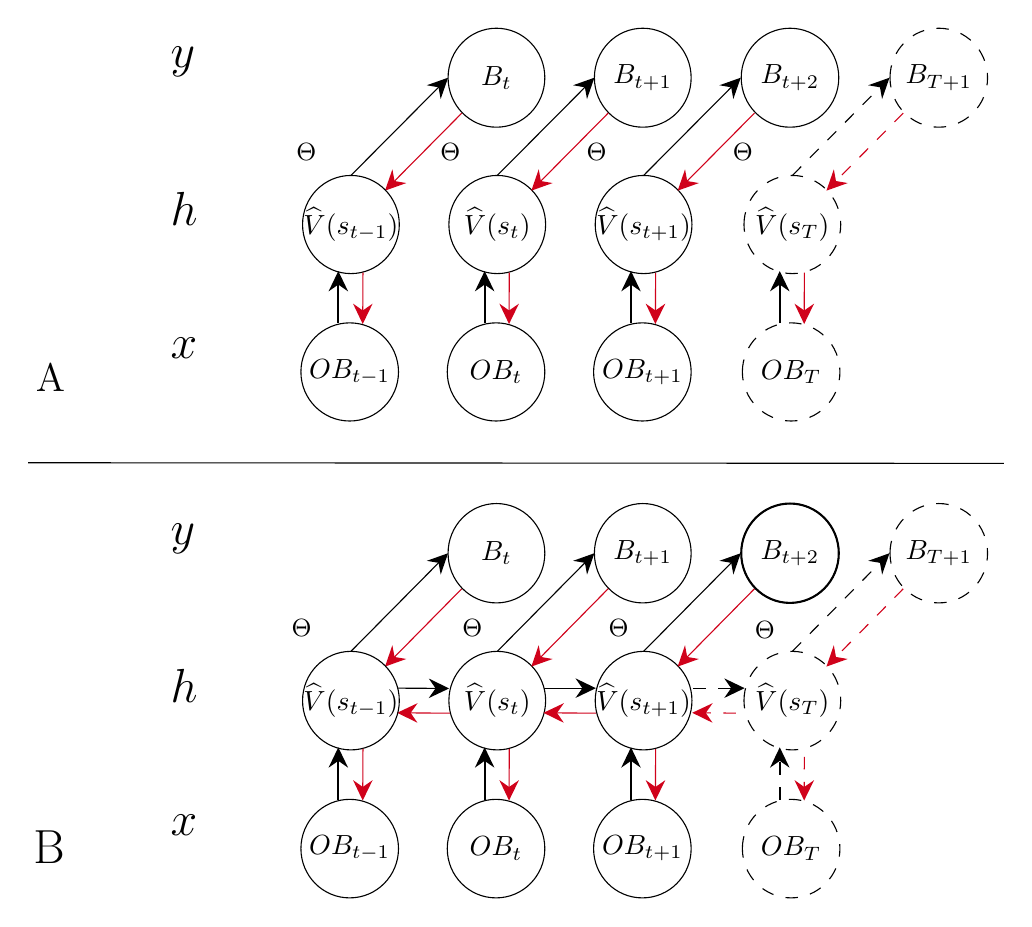
\begin{tikzpicture}[x=0.75pt,y=0.75pt,yscale=-1,xscale=1]
    %uncomment if require: \path (0,432); %set diagram left start at 0, and has height of 432
    
    %Shape: Ellipse [id:dp9152556376471453] 
    \draw   (252.87,325.26) .. controls (252.87,312.15) and (263.3,301.52) .. (276.18,301.52) .. controls (289.05,301.52) and (299.48,312.15) .. (299.48,325.26) .. controls (299.48,338.37) and (289.05,349) .. (276.18,349) .. controls (263.3,349) and (252.87,338.37) .. (252.87,325.26) -- cycle ;
    %Straight Lines [id:da0084456304461753] 
    \draw [color={rgb, 255:red, 208; green, 2; blue, 27 }  ,draw opacity=1 ]   (230.94,331.15) -- (253.32,331.31) ;
    \draw [shift={(227.94,331.12)}, rotate = 0.43] [fill={rgb, 255:red, 208; green, 2; blue, 27 }  ,fill opacity=1 ][line width=0.08]  [draw opacity=0] (9.82,-4.72) -- (0,0) -- (9.82,4.72) -- (6.52,0) -- cycle    ;
    %Shape: Ellipse [id:dp18326344407352502] 
    \draw   (181.58,396.56) .. controls (181.58,383.45) and (192.11,372.82) .. (205.08,372.82) .. controls (218.06,372.82) and (228.59,383.45) .. (228.59,396.56) .. controls (228.59,409.67) and (218.06,420.3) .. (205.08,420.3) .. controls (192.11,420.3) and (181.58,409.67) .. (181.58,396.56) -- cycle ;
    %Shape: Ellipse [id:dp4732045107682973] 
    \draw   (252.09,396.56) .. controls (252.09,383.45) and (262.61,372.82) .. (275.59,372.82) .. controls (288.57,372.82) and (299.09,383.45) .. (299.09,396.56) .. controls (299.09,409.67) and (288.57,420.3) .. (275.59,420.3) .. controls (262.61,420.3) and (252.09,409.67) .. (252.09,396.56) -- cycle ;
    %Straight Lines [id:da9106304988340169] 
    \draw    (205.67,301.52) -- (250.37,256.37) ;
    \draw [shift={(252.48,254.24)}, rotate = 494.71] [fill={rgb, 255:red, 0; green, 0; blue, 0 }  ][line width=0.08]  [draw opacity=0] (9.82,-4.72) -- (0,0) -- (9.82,4.72) -- (6.52,0) -- cycle    ;
    %Straight Lines [id:da5186602107869037] 
    \draw [color={rgb, 255:red, 208; green, 2; blue, 27 }  ,draw opacity=1 ]   (259.09,271.36) -- (224.2,306.73) ;
    \draw [shift={(222.1,308.86)}, rotate = 314.62] [fill={rgb, 255:red, 208; green, 2; blue, 27 }  ,fill opacity=1 ][line width=0.08]  [draw opacity=0] (9.82,-4.72) -- (0,0) -- (9.82,4.72) -- (6.52,0) -- cycle    ;
    %Shape: Ellipse [id:dp6434768624828036] 
    \draw   (322.59,396.56) .. controls (322.59,383.45) and (333.11,372.82) .. (346.09,372.82) .. controls (359.07,372.82) and (369.59,383.45) .. (369.59,396.56) .. controls (369.59,409.67) and (359.07,420.3) .. (346.09,420.3) .. controls (333.11,420.3) and (322.59,409.67) .. (322.59,396.56) -- cycle ;
    %Shape: Ellipse [id:dp4847846412537088] 
    \draw   (252.48,254.24) .. controls (252.48,241.02) and (262.91,230.3) .. (275.78,230.3) .. controls (288.65,230.3) and (299.09,241.02) .. (299.09,254.24) .. controls (299.09,267.46) and (288.65,278.18) .. (275.78,278.18) .. controls (262.91,278.18) and (252.48,267.46) .. (252.48,254.24) -- cycle ;
    %Shape: Ellipse [id:dp07973567399208026] 
    \draw   (322.98,254.24) .. controls (322.98,241.02) and (333.42,230.3) .. (346.29,230.3) .. controls (359.16,230.3) and (369.59,241.02) .. (369.59,254.24) .. controls (369.59,267.46) and (359.16,278.18) .. (346.29,278.18) .. controls (333.42,278.18) and (322.98,267.46) .. (322.98,254.24) -- cycle ;
    %Shape: Ellipse [id:dp05423142626898558] 
    \draw   (393.72,254.24) .. controls (393.72,241.02) and (404.24,230.3) .. (417.22,230.3) .. controls (430.2,230.3) and (440.72,241.02) .. (440.72,254.24) .. controls (440.72,267.46) and (430.2,278.18) .. (417.22,278.18) .. controls (404.24,278.18) and (393.72,267.46) .. (393.72,254.24) -- cycle ;
    %Shape: Ellipse [id:dp22782348689960996] 
    \draw   (182.37,325.26) .. controls (182.37,312.15) and (192.8,301.52) .. (205.67,301.52) .. controls (218.54,301.52) and (228.98,312.15) .. (228.98,325.26) .. controls (228.98,338.37) and (218.54,349) .. (205.67,349) .. controls (192.8,349) and (182.37,338.37) .. (182.37,325.26) -- cycle ;
    %Straight Lines [id:da8044112442211012] 
    \draw [line width=0.75]    (270.1,372.91) -- (270.1,350.76) ;
    \draw [shift={(270.1,347.76)}, rotate = 450] [fill={rgb, 255:red, 0; green, 0; blue, 0 }  ][line width=0.08]  [draw opacity=0] (9.82,-4.72) -- (0,0) -- (9.82,4.72) -- (6.52,0) -- cycle    ;
    %Straight Lines [id:da4352361095595384] 
    \draw [color={rgb, 255:red, 208; green, 2; blue, 27 }  ,draw opacity=1 ]   (281.87,370.38) -- (281.97,348.47) ;
    \draw [shift={(281.85,373.38)}, rotate = 270.27] [fill={rgb, 255:red, 208; green, 2; blue, 27 }  ,fill opacity=1 ][line width=0.08]  [draw opacity=0] (9.82,-4.72) -- (0,0) -- (9.82,4.72) -- (6.52,0) -- cycle    ;
    %Straight Lines [id:da9840961706533492] 
    \draw [color={rgb, 255:red, 0; green, 0; blue, 0 }  ,draw opacity=1 ]   (228.41,319.25) -- (249.98,319.36) ;
    \draw [shift={(252.98,319.38)}, rotate = 180.28] [fill={rgb, 255:red, 0; green, 0; blue, 0 }  ,fill opacity=1 ][line width=0.08]  [draw opacity=0] (9.82,-4.72) -- (0,0) -- (9.82,4.72) -- (6.52,0) -- cycle    ;
    %Straight Lines [id:da9105454079139469] 
    \draw [line width=0.75]    (340.61,372.91) -- (340.61,350.76) ;
    \draw [shift={(340.61,347.76)}, rotate = 450] [fill={rgb, 255:red, 0; green, 0; blue, 0 }  ][line width=0.08]  [draw opacity=0] (9.82,-4.72) -- (0,0) -- (9.82,4.72) -- (6.52,0) -- cycle    ;
    %Straight Lines [id:da2563913907740285] 
    \draw [color={rgb, 255:red, 208; green, 2; blue, 27 }  ,draw opacity=1 ]   (352.37,370.38) -- (352.48,348.47) ;
    \draw [shift={(352.36,373.38)}, rotate = 270.27] [fill={rgb, 255:red, 208; green, 2; blue, 27 }  ,fill opacity=1 ][line width=0.08]  [draw opacity=0] (9.82,-4.72) -- (0,0) -- (9.82,4.72) -- (6.52,0) -- cycle    ;
    %Shape: Ellipse [id:dp3682545800349367] 
    \draw   (323.37,325.26) .. controls (323.37,312.15) and (333.81,301.52) .. (346.68,301.52) .. controls (359.55,301.52) and (369.98,312.15) .. (369.98,325.26) .. controls (369.98,338.37) and (359.55,349) .. (346.68,349) .. controls (333.81,349) and (323.37,338.37) .. (323.37,325.26) -- cycle ;
    %Straight Lines [id:da5491729665822646] 
    \draw [line width=0.75]    (199.6,372.91) -- (199.6,350.76) ;
    \draw [shift={(199.6,347.76)}, rotate = 450] [fill={rgb, 255:red, 0; green, 0; blue, 0 }  ][line width=0.08]  [draw opacity=0] (9.82,-4.72) -- (0,0) -- (9.82,4.72) -- (6.52,0) -- cycle    ;
    %Straight Lines [id:da6906936296691885] 
    \draw [color={rgb, 255:red, 208; green, 2; blue, 27 }  ,draw opacity=1 ]   (211.37,370.38) -- (211.47,348.47) ;
    \draw [shift={(211.35,373.38)}, rotate = 270.27] [fill={rgb, 255:red, 208; green, 2; blue, 27 }  ,fill opacity=1 ][line width=0.08]  [draw opacity=0] (9.82,-4.72) -- (0,0) -- (9.82,4.72) -- (6.52,0) -- cycle    ;
    %Straight Lines [id:da8976403312606693] 
    \draw [color={rgb, 255:red, 208; green, 2; blue, 27 }  ,draw opacity=1 ]   (301.45,331.15) -- (323.82,331.31) ;
    \draw [shift={(298.45,331.12)}, rotate = 0.43] [fill={rgb, 255:red, 208; green, 2; blue, 27 }  ,fill opacity=1 ][line width=0.08]  [draw opacity=0] (9.82,-4.72) -- (0,0) -- (9.82,4.72) -- (6.52,0) -- cycle    ;
    %Straight Lines [id:da7873502214297404] 
    \draw [color={rgb, 255:red, 0; green, 0; blue, 0 }  ,draw opacity=1 ]   (298.92,319.25) -- (320.69,319.25) ;
    \draw [shift={(323.69,319.25)}, rotate = 180] [fill={rgb, 255:red, 0; green, 0; blue, 0 }  ,fill opacity=1 ][line width=0.08]  [draw opacity=0] (9.82,-4.72) -- (0,0) -- (9.82,4.72) -- (6.52,0) -- cycle    ;
    %Straight Lines [id:da38615546041268245] 
    \draw    (276.18,301.52) -- (320.87,256.37) ;
    \draw [shift={(322.98,254.24)}, rotate = 494.71] [fill={rgb, 255:red, 0; green, 0; blue, 0 }  ][line width=0.08]  [draw opacity=0] (9.82,-4.72) -- (0,0) -- (9.82,4.72) -- (6.52,0) -- cycle    ;
    %Straight Lines [id:da8727709104298054] 
    \draw [color={rgb, 255:red, 208; green, 2; blue, 27 }  ,draw opacity=1 ]   (329.6,271.36) -- (294.71,306.73) ;
    \draw [shift={(292.6,308.86)}, rotate = 314.62] [fill={rgb, 255:red, 208; green, 2; blue, 27 }  ,fill opacity=1 ][line width=0.08]  [draw opacity=0] (9.82,-4.72) -- (0,0) -- (9.82,4.72) -- (6.52,0) -- cycle    ;
    %Straight Lines [id:da025606451942667974] 
    \draw    (346.68,301.52) -- (391.37,256.37) ;
    \draw [shift={(393.48,254.24)}, rotate = 494.71] [fill={rgb, 255:red, 0; green, 0; blue, 0 }  ][line width=0.08]  [draw opacity=0] (9.82,-4.72) -- (0,0) -- (9.82,4.72) -- (6.52,0) -- cycle    ;
    %Straight Lines [id:da7157498693904918] 
    \draw [color={rgb, 255:red, 208; green, 2; blue, 27 }  ,draw opacity=1 ]   (400.1,271.36) -- (365.21,306.73) ;
    \draw [shift={(363.1,308.86)}, rotate = 314.62] [fill={rgb, 255:red, 208; green, 2; blue, 27 }  ,fill opacity=1 ][line width=0.08]  [draw opacity=0] (9.82,-4.72) -- (0,0) -- (9.82,4.72) -- (6.52,0) -- cycle    ;
    %Shape: Ellipse [id:dp1944088973906778] 
    \draw   (252.87,95.88) .. controls (252.87,82.82) and (263.3,72.23) .. (276.18,72.23) .. controls (289.05,72.23) and (299.48,82.82) .. (299.48,95.88) .. controls (299.48,108.94) and (289.05,119.52) .. (276.18,119.52) .. controls (263.3,119.52) and (252.87,108.94) .. (252.87,95.88) -- cycle ;
    %Shape: Ellipse [id:dp7540301212468546] 
    \draw   (181.58,166.89) .. controls (181.58,153.83) and (192.11,143.25) .. (205.08,143.25) .. controls (218.06,143.25) and (228.59,153.83) .. (228.59,166.89) .. controls (228.59,179.95) and (218.06,190.54) .. (205.08,190.54) .. controls (192.11,190.54) and (181.58,179.95) .. (181.58,166.89) -- cycle ;
    %Shape: Ellipse [id:dp5780436923676984] 
    \draw   (252.09,166.89) .. controls (252.09,153.83) and (262.61,143.25) .. (275.59,143.25) .. controls (288.57,143.25) and (299.09,153.83) .. (299.09,166.89) .. controls (299.09,179.95) and (288.57,190.54) .. (275.59,190.54) .. controls (262.61,190.54) and (252.09,179.95) .. (252.09,166.89) -- cycle ;
    %Straight Lines [id:da6776717368806907] 
    \draw    (205.67,72.23) -- (250.36,27.27) ;
    \draw [shift={(252.48,25.14)}, rotate = 494.83] [fill={rgb, 255:red, 0; green, 0; blue, 0 }  ][line width=0.08]  [draw opacity=0] (9.82,-4.72) -- (0,0) -- (9.82,4.72) -- (6.52,0) -- cycle    ;
    %Straight Lines [id:da030655313121066063] 
    \draw [color={rgb, 255:red, 208; green, 2; blue, 27 }  ,draw opacity=1 ]   (259.09,42.2) -- (224.21,77.42) ;
    \draw [shift={(222.1,79.55)}, rotate = 314.73] [fill={rgb, 255:red, 208; green, 2; blue, 27 }  ,fill opacity=1 ][line width=0.08]  [draw opacity=0] (9.82,-4.72) -- (0,0) -- (9.82,4.72) -- (6.52,0) -- cycle    ;
    %Shape: Ellipse [id:dp9167477381870462] 
    \draw   (322.59,166.89) .. controls (322.59,153.83) and (333.11,143.25) .. (346.09,143.25) .. controls (359.07,143.25) and (369.59,153.83) .. (369.59,166.89) .. controls (369.59,179.95) and (359.07,190.54) .. (346.09,190.54) .. controls (333.11,190.54) and (322.59,179.95) .. (322.59,166.89) -- cycle ;
    %Shape: Ellipse [id:dp28076940126490224] 
    \draw   (252.48,25.14) .. controls (252.48,11.97) and (262.91,1.3) .. (275.78,1.3) .. controls (288.65,1.3) and (299.09,11.97) .. (299.09,25.14) .. controls (299.09,38.31) and (288.65,48.98) .. (275.78,48.98) .. controls (262.91,48.98) and (252.48,38.31) .. (252.48,25.14) -- cycle ;
    %Shape: Ellipse [id:dp018136489069107253] 
    \draw   (322.98,25.14) .. controls (322.98,11.97) and (333.42,1.3) .. (346.29,1.3) .. controls (359.16,1.3) and (369.59,11.97) .. (369.59,25.14) .. controls (369.59,38.31) and (359.16,48.98) .. (346.29,48.98) .. controls (333.42,48.98) and (322.98,38.31) .. (322.98,25.14) -- cycle ;
    %Shape: Ellipse [id:dp43337791741971476] 
    \draw   (393.72,25.14) .. controls (393.72,11.97) and (404.24,1.3) .. (417.22,1.3) .. controls (430.2,1.3) and (440.72,11.97) .. (440.72,25.14) .. controls (440.72,38.31) and (430.2,48.98) .. (417.22,48.98) .. controls (404.24,48.98) and (393.72,38.31) .. (393.72,25.14) -- cycle ;
    %Shape: Ellipse [id:dp27462372888763276] 
    \draw   (182.37,95.88) .. controls (182.37,82.82) and (192.8,72.23) .. (205.67,72.23) .. controls (218.54,72.23) and (228.98,82.82) .. (228.98,95.88) .. controls (228.98,108.94) and (218.54,119.52) .. (205.67,119.52) .. controls (192.8,119.52) and (182.37,108.94) .. (182.37,95.88) -- cycle ;
    %Straight Lines [id:da29813692702208516] 
    \draw [line width=0.75]    (270.1,143.33) -- (270.1,121.29) ;
    \draw [shift={(270.1,118.29)}, rotate = 450] [fill={rgb, 255:red, 0; green, 0; blue, 0 }  ][line width=0.08]  [draw opacity=0] (9.82,-4.72) -- (0,0) -- (9.82,4.72) -- (6.52,0) -- cycle    ;
    %Straight Lines [id:da3349478757051123] 
    \draw [color={rgb, 255:red, 208; green, 2; blue, 27 }  ,draw opacity=1 ]   (281.87,140.81) -- (281.97,118.99) ;
    \draw [shift={(281.85,143.81)}, rotate = 270.27] [fill={rgb, 255:red, 208; green, 2; blue, 27 }  ,fill opacity=1 ][line width=0.08]  [draw opacity=0] (9.82,-4.72) -- (0,0) -- (9.82,4.72) -- (6.52,0) -- cycle    ;
    %Straight Lines [id:da9602295578636938] 
    \draw [line width=0.75]    (340.61,143.33) -- (340.61,121.29) ;
    \draw [shift={(340.61,118.29)}, rotate = 450] [fill={rgb, 255:red, 0; green, 0; blue, 0 }  ][line width=0.08]  [draw opacity=0] (9.82,-4.72) -- (0,0) -- (9.82,4.72) -- (6.52,0) -- cycle    ;
    %Straight Lines [id:da63886615565973] 
    \draw [color={rgb, 255:red, 208; green, 2; blue, 27 }  ,draw opacity=1 ]   (352.37,140.81) -- (352.48,118.99) ;
    \draw [shift={(352.36,143.81)}, rotate = 270.27] [fill={rgb, 255:red, 208; green, 2; blue, 27 }  ,fill opacity=1 ][line width=0.08]  [draw opacity=0] (9.82,-4.72) -- (0,0) -- (9.82,4.72) -- (6.52,0) -- cycle    ;
    %Shape: Ellipse [id:dp8361207322156409] 
    \draw   (323.37,95.88) .. controls (323.37,82.82) and (333.81,72.23) .. (346.68,72.23) .. controls (359.55,72.23) and (369.98,82.82) .. (369.98,95.88) .. controls (369.98,108.94) and (359.55,119.52) .. (346.68,119.52) .. controls (333.81,119.52) and (323.37,108.94) .. (323.37,95.88) -- cycle ;
    %Straight Lines [id:da4551016346165171] 
    \draw [line width=0.75]    (199.6,143.33) -- (199.6,121.29) ;
    \draw [shift={(199.6,118.29)}, rotate = 450] [fill={rgb, 255:red, 0; green, 0; blue, 0 }  ][line width=0.08]  [draw opacity=0] (9.82,-4.72) -- (0,0) -- (9.82,4.72) -- (6.52,0) -- cycle    ;
    %Straight Lines [id:da561902479346039] 
    \draw [color={rgb, 255:red, 208; green, 2; blue, 27 }  ,draw opacity=1 ]   (211.37,140.81) -- (211.47,118.99) ;
    \draw [shift={(211.35,143.81)}, rotate = 270.27] [fill={rgb, 255:red, 208; green, 2; blue, 27 }  ,fill opacity=1 ][line width=0.08]  [draw opacity=0] (9.82,-4.72) -- (0,0) -- (9.82,4.72) -- (6.52,0) -- cycle    ;
    %Straight Lines [id:da8478794915247372] 
    \draw    (276.18,72.23) -- (320.87,27.27) ;
    \draw [shift={(322.98,25.14)}, rotate = 494.83] [fill={rgb, 255:red, 0; green, 0; blue, 0 }  ][line width=0.08]  [draw opacity=0] (9.82,-4.72) -- (0,0) -- (9.82,4.72) -- (6.52,0) -- cycle    ;
    %Straight Lines [id:da27798944049873586] 
    \draw [color={rgb, 255:red, 208; green, 2; blue, 27 }  ,draw opacity=1 ]   (329.6,42.2) -- (294.71,77.42) ;
    \draw [shift={(292.6,79.55)}, rotate = 314.73] [fill={rgb, 255:red, 208; green, 2; blue, 27 }  ,fill opacity=1 ][line width=0.08]  [draw opacity=0] (9.82,-4.72) -- (0,0) -- (9.82,4.72) -- (6.52,0) -- cycle    ;
    %Straight Lines [id:da24137509475938523] 
    \draw    (346.68,72.23) -- (391.37,27.27) ;
    \draw [shift={(393.48,25.14)}, rotate = 494.83] [fill={rgb, 255:red, 0; green, 0; blue, 0 }  ][line width=0.08]  [draw opacity=0] (9.82,-4.72) -- (0,0) -- (9.82,4.72) -- (6.52,0) -- cycle    ;
    %Straight Lines [id:da5361482602236827] 
    \draw [color={rgb, 255:red, 208; green, 2; blue, 27 }  ,draw opacity=1 ]   (400.1,42.2) -- (365.21,77.42) ;
    \draw [shift={(363.1,79.55)}, rotate = 314.73] [fill={rgb, 255:red, 208; green, 2; blue, 27 }  ,fill opacity=1 ][line width=0.08]  [draw opacity=0] (9.82,-4.72) -- (0,0) -- (9.82,4.72) -- (6.52,0) -- cycle    ;
    %Shape: Ellipse [id:dp9428082939545759] 
    \draw  [dash pattern={on 4.5pt off 4.5pt}] (394.27,166.89) .. controls (394.27,153.83) and (404.79,143.25) .. (417.77,143.25) .. controls (430.75,143.25) and (441.27,153.83) .. (441.27,166.89) .. controls (441.27,179.95) and (430.75,190.54) .. (417.77,190.54) .. controls (404.79,190.54) and (394.27,179.95) .. (394.27,166.89) -- cycle ;
    %Shape: Ellipse [id:dp12638273249032017] 
    \draw  [dash pattern={on 4.5pt off 4.5pt}] (465.4,25.14) .. controls (465.4,11.97) and (475.92,1.3) .. (488.9,1.3) .. controls (501.88,1.3) and (512.4,11.97) .. (512.4,25.14) .. controls (512.4,38.31) and (501.88,48.98) .. (488.9,48.98) .. controls (475.92,48.98) and (465.4,38.31) .. (465.4,25.14) -- cycle ;
    %Shape: Ellipse [id:dp8917959348395956] 
    \draw  [dash pattern={on 4.5pt off 4.5pt}] (395.05,95.88) .. controls (395.05,82.82) and (405.49,72.23) .. (418.36,72.23) .. controls (431.23,72.23) and (441.66,82.82) .. (441.66,95.88) .. controls (441.66,108.94) and (431.23,119.52) .. (418.36,119.52) .. controls (405.49,119.52) and (395.05,108.94) .. (395.05,95.88) -- cycle ;
    %Straight Lines [id:da6091521843857648] 
    \draw  [dash pattern={on 4.5pt off 4.5pt}]  (418.36,72.23) -- (463.05,27.27) ;
    \draw [shift={(465.16,25.14)}, rotate = 494.83] [fill={rgb, 255:red, 0; green, 0; blue, 0 }  ][line width=0.08]  [draw opacity=0] (9.82,-4.72) -- (0,0) -- (9.82,4.72) -- (6.52,0) -- cycle    ;
    %Straight Lines [id:da18105258004250324] 
    \draw [color={rgb, 255:red, 208; green, 2; blue, 27 }  ,draw opacity=1 ] [dash pattern={on 4.5pt off 4.5pt}]  (471.78,42.2) -- (436.89,77.42) ;
    \draw [shift={(434.78,79.55)}, rotate = 314.73] [fill={rgb, 255:red, 208; green, 2; blue, 27 }  ,fill opacity=1 ][line width=0.08]  [draw opacity=0] (9.82,-4.72) -- (0,0) -- (9.82,4.72) -- (6.52,0) -- cycle    ;
    %Straight Lines [id:da6760788428742098] 
    \draw [line width=0.75]    (412.29,143.33) -- (412.29,121.29) ;
    \draw [shift={(412.29,118.29)}, rotate = 450] [fill={rgb, 255:red, 0; green, 0; blue, 0 }  ][line width=0.08]  [draw opacity=0] (9.82,-4.72) -- (0,0) -- (9.82,4.72) -- (6.52,0) -- cycle    ;
    %Straight Lines [id:da7825592771106329] 
    \draw [color={rgb, 255:red, 208; green, 2; blue, 27 }  ,draw opacity=1 ]   (424.05,140.81) -- (424.15,118.99) ;
    \draw [shift={(424.04,143.81)}, rotate = 270.27] [fill={rgb, 255:red, 208; green, 2; blue, 27 }  ,fill opacity=1 ][line width=0.08]  [draw opacity=0] (9.82,-4.72) -- (0,0) -- (9.82,4.72) -- (6.52,0) -- cycle    ;
    %Shape: Ellipse [id:dp44556831775872074] 
    \draw  [line width=0.75]  (393.72,254.24) .. controls (393.72,241.02) and (404.24,230.3) .. (417.22,230.3) .. controls (430.2,230.3) and (440.72,241.02) .. (440.72,254.24) .. controls (440.72,267.46) and (430.2,278.18) .. (417.22,278.18) .. controls (404.24,278.18) and (393.72,267.46) .. (393.72,254.24) -- cycle ;
    %Shape: Ellipse [id:dp001475416847050881] 
    \draw  [dash pattern={on 4.5pt off 4.5pt}] (394.27,396.56) .. controls (394.27,383.45) and (404.79,372.82) .. (417.77,372.82) .. controls (430.75,372.82) and (441.27,383.45) .. (441.27,396.56) .. controls (441.27,409.67) and (430.75,420.3) .. (417.77,420.3) .. controls (404.79,420.3) and (394.27,409.67) .. (394.27,396.56) -- cycle ;
    %Shape: Ellipse [id:dp6004502309758961] 
    \draw  [dash pattern={on 4.5pt off 4.5pt}] (465.4,254.24) .. controls (465.4,241.02) and (475.92,230.3) .. (488.9,230.3) .. controls (501.88,230.3) and (512.4,241.02) .. (512.4,254.24) .. controls (512.4,267.46) and (501.88,278.18) .. (488.9,278.18) .. controls (475.92,278.18) and (465.4,267.46) .. (465.4,254.24) -- cycle ;
    %Shape: Ellipse [id:dp9012578897389621] 
    \draw  [dash pattern={on 4.5pt off 4.5pt}] (395.05,325.26) .. controls (395.05,312.15) and (405.49,301.52) .. (418.36,301.52) .. controls (431.23,301.52) and (441.66,312.15) .. (441.66,325.26) .. controls (441.66,338.37) and (431.23,349) .. (418.36,349) .. controls (405.49,349) and (395.05,338.37) .. (395.05,325.26) -- cycle ;
    %Straight Lines [id:da8776948176349402] 
    \draw  [dash pattern={on 4.5pt off 4.5pt}]  (418.36,301.52) -- (463.05,256.37) ;
    \draw [shift={(465.16,254.24)}, rotate = 494.71] [fill={rgb, 255:red, 0; green, 0; blue, 0 }  ][line width=0.08]  [draw opacity=0] (9.82,-4.72) -- (0,0) -- (9.82,4.72) -- (6.52,0) -- cycle    ;
    %Straight Lines [id:da11237121474720091] 
    \draw [color={rgb, 255:red, 208; green, 2; blue, 27 }  ,draw opacity=1 ] [dash pattern={on 4.5pt off 4.5pt}]  (471.78,271.36) -- (436.89,306.73) ;
    \draw [shift={(434.78,308.86)}, rotate = 314.62] [fill={rgb, 255:red, 208; green, 2; blue, 27 }  ,fill opacity=1 ][line width=0.08]  [draw opacity=0] (9.82,-4.72) -- (0,0) -- (9.82,4.72) -- (6.52,0) -- cycle    ;
    %Straight Lines [id:da12172698001213589] 
    \draw [line width=0.75]  [dash pattern={on 4.5pt off 4.5pt}]  (412.29,372.91) -- (412.29,350.76) ;
    \draw [shift={(412.29,347.76)}, rotate = 450] [fill={rgb, 255:red, 0; green, 0; blue, 0 }  ][line width=0.08]  [draw opacity=0] (9.82,-4.72) -- (0,0) -- (9.82,4.72) -- (6.52,0) -- cycle    ;
    %Straight Lines [id:da6444397198631048] 
    \draw [color={rgb, 255:red, 208; green, 2; blue, 27 }  ,draw opacity=1 ] [dash pattern={on 4.5pt off 4.5pt}]  (424.05,370.38) -- (424.15,348.47) ;
    \draw [shift={(424.04,373.38)}, rotate = 270.27] [fill={rgb, 255:red, 208; green, 2; blue, 27 }  ,fill opacity=1 ][line width=0.08]  [draw opacity=0] (9.82,-4.72) -- (0,0) -- (9.82,4.72) -- (6.52,0) -- cycle    ;
    %Straight Lines [id:da11944678601617786] 
    \draw [color={rgb, 255:red, 208; green, 2; blue, 27 }  ,draw opacity=1 ] [dash pattern={on 4.5pt off 4.5pt}]  (373.12,331.15) -- (395.5,331.31) ;
    \draw [shift={(370.12,331.12)}, rotate = 0.43] [fill={rgb, 255:red, 208; green, 2; blue, 27 }  ,fill opacity=1 ][line width=0.08]  [draw opacity=0] (9.82,-4.72) -- (0,0) -- (9.82,4.72) -- (6.52,0) -- cycle    ;
    %Straight Lines [id:da6070445313661826] 
    \draw [color={rgb, 255:red, 0; green, 0; blue, 0 }  ,draw opacity=1 ] [dash pattern={on 4.5pt off 4.5pt}]  (370.59,319.25) -- (392.36,319.25) ;
    \draw [shift={(395.36,319.25)}, rotate = 180] [fill={rgb, 255:red, 0; green, 0; blue, 0 }  ,fill opacity=1 ][line width=0.08]  [draw opacity=0] (9.82,-4.72) -- (0,0) -- (9.82,4.72) -- (6.52,0) -- cycle    ;
    %Straight Lines [id:da8091605227382529] 
    \draw    (50.2,210.65) -- (520.2,210.95) ;
    
    % Text Node
    \draw (51.39,386.85) node [anchor=north west][inner sep=0.75pt]   [align=left] {{\LARGE B}};
    % Text Node
    \draw (205.08,396.56) node    {$OB_{t-1}$};
    % Text Node
    \draw (205.67,325.26) node    {$\widehat{V}(s_{t-1})$};
    % Text Node
    \draw (275.59,396.56) node    {$OB_{t}$};
    % Text Node
    \draw (276.18,325.26) node    {$\widehat{V}(s_t)$};
    % Text Node
    \draw (275.78,254.24) node    {$B_{t}$};
    % Text Node
    \draw (346.09,396.56) node  [font=\normalsize]  {$OB_{t+1}$};
    % Text Node
    \draw (346.68,325.26) node    {$\widehat{V}(s_{t+1})$};
    % Text Node
    \draw (346.29,254.24) node    {$B_{t+1}$};
    % Text Node
    \draw (417.22,254.24) node    {$B_{t+2}$};
    % Text Node
    \draw (181.86,290.07) node  [font=\small]  {$\Theta$};
    % Text Node
    \draw (264.11,290.07) node  [font=\small]  {$\Theta$};
    % Text Node
    \draw (334.61,290.07) node  [font=\small]  {$\Theta$};
    % Text Node
    \draw (205.08,166.89) node    {$OB_{t-1}$};
    % Text Node
    \draw (205.67,95.88) node    {$\widehat{V}(s_{t-1})$};
    % Text Node
    \draw (275.59,166.89) node    {$OB_{t}$};
    % Text Node
    \draw (276.18,95.88) node    {$\widehat{V}(s_{t})$};
    % Text Node
    \draw (275.78,25.14) node    {$B_{t}$};
    % Text Node
    \draw (346.09,166.89) node    {$OB_{t+1}$};
    % Text Node
    \draw (346.68,95.88) node    {$\widehat{V}(s_{t+1})$};
    % Text Node
    \draw (346.29,25.14) node    {$B_{t+1}$};
    % Text Node
    \draw (417.22,25.14) node    {$B_{t+2}$};
    % Text Node
    \draw (184.21,60.83) node  [font=\small]  {$\Theta $};
    % Text Node
    \draw (417.77,166.89) node    {$OB_{T}$};
    % Text Node
    \draw (418.36,95.88) node    {$\widehat{V}(s_{T})$};
    % Text Node
    \draw (488.9,25.14) node    {$B_{T+1}$};
    % Text Node
    \draw (52.57,162.08) node [anchor=north west][inner sep=0.75pt]   [align=left] {{\Large A}};
    % Text Node
    \draw (417.77,396.56) node    {$OB_{T}$};
    % Text Node
    \draw (418.36,325.26) node    {$\widehat{V}(s_{T})$};
    % Text Node
    \draw (488.9,254.24) node    {$B_{T+1}$};
    % Text Node
    \draw (405.12,291.26) node  [font=\small]  {$\Theta$};
    % Text Node
    \draw (253.54,60.83) node  [font=\small]  {$\Theta$};
    % Text Node
    \draw (324.04,60.83) node  [font=\small]  {$\Theta$};
    % Text Node
    \draw (394.54,60.83) node  [font=\small]  {$\Theta$};
    % Text Node
    \draw (117.57,9.08) node [anchor=north west][inner sep=0.75pt]  [font=\LARGE] [align=left] {$\displaystyle y$};
    % Text Node
    \draw (117.57,79.08) node [anchor=north west][inner sep=0.75pt]  [font=\LARGE] [align=left] {$\displaystyle h$};
    % Text Node
    \draw (117.57,149.08) node [anchor=north west][inner sep=0.75pt]  [font=\LARGE] [align=left] {$\displaystyle x$};
    % Text Node
    \draw (117.57,239.08) node [anchor=north west][inner sep=0.75pt]  [font=\LARGE] [align=left] {$\displaystyle y$};
    % Text Node
    \draw (117.57,309.08) node [anchor=north west][inner sep=0.75pt]  [font=\LARGE] [align=left] {$\displaystyle h$};
    % Text Node
    \draw (117.57,379.08) node [anchor=north west][inner sep=0.75pt]  [font=\LARGE] [align=left] {$\displaystyle x$};

    \end{tikzpicture}
\end{adjustbox}
\end{center}

\caption{\textbf{Differences in single-step prediction between feed-forward (A) and recurrent (B) neural networks}. Adapted from \cite{bengio2017deep,lillicrap2019backpropagation}, the figure represents how feedforward and recurrent ANNs could be used for estimating $V(s_t)$. Here $OB=\{OB_{t}: t \in T\}$ indicates the series of inputs of length $T$  that the network receives while the target is the lead 1 version of the $B$ portion of the same series. The series $\widehat{V}=\{\widehat{V}(s_{t}): t \in T\}$ correspond to the representations generated combining the input with the parameters $\Theta$ learned by the network in order to approximate the target. Circles indicate computational blocks similar to those present in figure \ref{fig: ffnn}. Black and red arrows are respectively the direction of the computations and the flow of the error gradient.}
\label{fig: ffnn_rnn}
\end{figure}

\subsection{Representation and Manifold Learning}
\label{manifold_learning}
As mentioned in the previous sections, ANNs are tasked to create latent representations (e.g. $V(s_{t})$) which are not explicitly defined by their input or target but are nevertheless functional for connecting the two \cite{rumelhart1986learning,bengio2017deep,lillicrap2020backpropagation}. This is based on the hypothesis that the relationship between the input and the target can be expressed in terms of variations in coordinates on a manifold \cite{bengio2017deep}. In the lower dimensional space of this manifold, the input is re-organized to improve estimation and elements which are similar to each other tend to appear close together \cite{bengio2017deep}. In this view, during optimization, each layer of an ANN attempts to place its input on a manifold that is useful for the layer that follows. This process continues until the last layer. Here the inputs are organized in such way that it makes easier for the network to produce good predictions of the target \cite{bengio2017deep}. Moving along this final manifold allows one to reach inputs with different characteristics leading to variations in the predictions produced by the model. We hypothesize that the amount of attributed incentive salience (i.e. $V(s_{t})$) can be modeled as a manifold on which the history of individual-object interactions is placed in order to best predict the intensity of all future interactions. This relates to the concept of motivation as a vector presented in sections \ref{motivation} and \ref{manifold_state}: the representation $V(s_{t})$ estimated by an ANN can be thought of as a vector in an $h$ dimensional space, where $h$ is the number of units of the layer producing the representation, indicating the amount of attributed incentive salience after observing $t$ interactions. As we can see, differently from completely un-supervised approaches this approach forces the learned manifold to obey to specific representational and predictive functionalities that are shared with the construct of attributed incentive salience. Given the potentially large number of layers in an ANN, locating this representation and most importantly ensuring that it is a suitable approximation of $V(s_{t})$ are potential issues. A possible solution is to impose a form of architectural constraint on the optimization process through multi-task learning. Multi-task learning closely resemble multivariate analysis, it  works on the assumption that a common latent factor underlying a set of targets exists and it can be constrained in a single representation used by the ANN for producing multiple predictions \cite{bengio2017deep}. An example of this process is shown in figure \ref{fig: multi_task}. As mentioned in section \ref{incentive_salience}, the amount of attributed incentive salience $V(s_t)$ that an individual $I$ assigns to an object $O$ should be a latent factor that indicates how intense future interactions with that object will be. Therefore, if a layer in an ANN is forced to produce a single representation which is then used to estimate multiple behavioural indicators of the intensity of these interactions, this should provide a sensible approximation of the amount of attributed incentive salience. 
\begin{figure}[h]
  \begin{center}
    \begin{adjustbox}{width=0.6\columnwidth}
        \tikzset{every picture/.style={line width=0.75pt}} %set default line width to 0.75pt        
        
        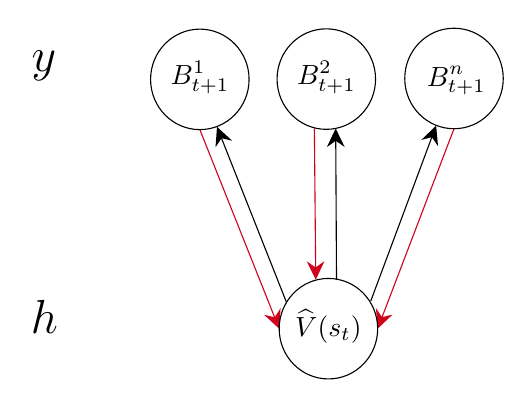
\begin{tikzpicture}[x=0.75pt,y=0.75pt,yscale=-1,xscale=1]
        %uncomment if require: \path (0,300); %set diagram left start at 0, and has height of 300
        
        %Straight Lines [id:da4267952151606098] 
        \draw    (319.82,122) -- (320.2,191.88) ;
        \draw [shift={(319.8,119)}, rotate = 89.69] [fill={rgb, 255:red, 0; green, 0; blue, 0 }  ][line width=0.08]  [draw opacity=0] (8.93,-4.29) -- (0,0) -- (8.93,4.29) -- (5.93,0) -- cycle    ;
        %Straight Lines [id:da6989378371909234] 
        \draw [color={rgb, 255:red, 208; green, 2; blue, 27 }  ,draw opacity=1 ]   (310.17,188.88) -- (309.53,119) ;
        \draw [shift={(310.2,191.88)}, rotate = 269.48] [fill={rgb, 255:red, 208; green, 2; blue, 27 }  ,fill opacity=1 ][line width=0.08]  [draw opacity=0] (8.93,-4.29) -- (0,0) -- (8.93,4.29) -- (5.93,0) -- cycle    ;
        %Shape: Ellipse [id:dp8707618719305075] 
        \draw   (353.08,94.91) .. controls (353.08,81.53) and (363.7,70.7) .. (376.81,70.7) .. controls (389.91,70.7) and (400.53,81.53) .. (400.53,94.91) .. controls (400.53,108.28) and (389.91,119.12) .. (376.81,119.12) .. controls (363.7,119.12) and (353.08,108.28) .. (353.08,94.91) -- cycle ;
        %Straight Lines [id:da13933094112344846] 
        \draw [color={rgb, 255:red, 208; green, 2; blue, 27 }  ,draw opacity=1 ]   (341.1,212.65) -- (376.81,119.12) ;
        \draw [shift={(340.03,215.46)}, rotate = 290.89] [fill={rgb, 255:red, 208; green, 2; blue, 27 }  ,fill opacity=1 ][line width=0.08]  [draw opacity=0] (8.93,-4.29) -- (0,0) -- (8.93,4.29) -- (5.93,0) -- cycle    ;
        %Shape: Ellipse [id:dp9097319337144372] 
        \draw   (291.56,95.2) .. controls (291.56,81.82) and (302.18,70.99) .. (315.29,70.99) .. controls (328.39,70.99) and (339.01,81.82) .. (339.01,95.2) .. controls (339.01,108.57) and (328.39,119.41) .. (315.29,119.41) .. controls (302.18,119.41) and (291.56,108.57) .. (291.56,95.2) -- cycle ;
        %Straight Lines [id:da3769355222150532] 
        \draw [color={rgb, 255:red, 208; green, 2; blue, 27 }  ,draw opacity=1 ]   (291.47,212.67) -- (254.35,119.55) ;
        \draw [shift={(292.58,215.46)}, rotate = 248.27] [fill={rgb, 255:red, 208; green, 2; blue, 27 }  ,fill opacity=1 ][line width=0.08]  [draw opacity=0] (8.93,-4.29) -- (0,0) -- (8.93,4.29) -- (5.93,0) -- cycle    ;
        %Straight Lines [id:da1253267073766362] 
        \draw [color={rgb, 255:red, 0; green, 0; blue, 0 }  ,draw opacity=1 ]   (263.71,120.96) -- (296.02,202.56) ;
        \draw [shift={(262.61,118.17)}, rotate = 68.4] [fill={rgb, 255:red, 0; green, 0; blue, 0 }  ,fill opacity=1 ][line width=0.08]  [draw opacity=0] (8.93,-4.29) -- (0,0) -- (8.93,4.29) -- (5.93,0) -- cycle    ;
        %Shape: Ellipse [id:dp7350394708339132] 
        \draw   (292.58,215.46) .. controls (292.58,202.09) and (303.2,191.25) .. (316.3,191.25) .. controls (329.41,191.25) and (340.03,202.09) .. (340.03,215.46) .. controls (340.03,228.83) and (329.41,239.67) .. (316.3,239.67) .. controls (303.2,239.67) and (292.58,228.83) .. (292.58,215.46) -- cycle ;
        %Shape: Ellipse [id:dp34753658855295044] 
        \draw   (230.62,95.34) .. controls (230.62,81.97) and (241.24,71.13) .. (254.35,71.13) .. controls (267.45,71.13) and (278.07,81.97) .. (278.07,95.34) .. controls (278.07,108.71) and (267.45,119.55) .. (254.35,119.55) .. controls (241.24,119.55) and (230.62,108.71) .. (230.62,95.34) -- cycle ;
        %Straight Lines [id:da6916637423351373] 
        \draw [color={rgb, 255:red, 0; green, 0; blue, 0 }  ,draw opacity=1 ]   (367.15,120.44) -- (336.7,202.13) ;
        \draw [shift={(368.2,117.63)}, rotate = 110.44] [fill={rgb, 255:red, 0; green, 0; blue, 0 }  ,fill opacity=1 ][line width=0.08]  [draw opacity=0] (8.93,-4.29) -- (0,0) -- (8.93,4.29) -- (5.93,0) -- cycle    ;
        
        % Text Node
        \draw (316.33,214.5) node   [align=left] {$\displaystyle \widehat{V}( s_{t})$};
        % Text Node
        \draw (254.43,94.4) node   [align=left] {$\displaystyle B^{1}_{t+1}$};
        % Text Node
        \draw (315.37,94.25) node   [align=left] {$\displaystyle B^{2}_{t+1}$};
        % Text Node
        \draw (377.91,95.99) node   [align=left] {$\displaystyle B^{n}_{t+1}$};
        % Text Node
        \draw (171.67,200.4) node [anchor=north west][inner sep=0.75pt]  [font=\LARGE]  {$h$};
        % Text Node
        \draw (172,80.4) node [anchor=north west][inner sep=0.75pt]  [font=\LARGE]  {$y$};
        
        \end{tikzpicture}
    \end{adjustbox}
\end{center}
\caption{\textbf{Multi-task learning in an ANN}. Adapted from \cite{bengio2017deep}. The figure represents how multi-task learning could be used in an ANN to force the the latent representation $h$ to be a sensible approximation of $V(s_t)$. Here $\widehat{V}(s_t)$ indicates the representation generated by a recurrent layer at time $t$ while $B_{t+1}=\{B^n_{t+1}: n \in N\}$ are $N$ targets quantifying the strength of the next interaction (in terms of frequency and amount of behaviour)  between $I$ and $O$. Black and red arrows are respectively the direction of the computations and the flow of the error gradient. Circles indicate computational blocks similar to those in figures \ref{fig: ffnn} and \ref{fig: ffnn_rnn}.}
\label{fig: multi_task}
\end{figure}

\chapter{Model Implementation and Testing}
\label{chapter_implementation_testing}
\section{Introduction}
\label{implementation_testing_introduction}

\section{Joint Prediction of Future Behavioural Intensity}
\label{model_architecture_1}

\subsection{Model Description}
We present a novel deep neural network architecture, loosely inspired by the winning entry in \cite{lee2018game}, for jointly estimate survival time and churn probability. This architecture, the `Bifurcating Model' (BM), is demonstrated in Fig. \ref{bm_architecture}. The model receives, as input, both a vector of unfolded features, as in Table \ref{metricsdescription}, as well as a context vector containing a numerical encoding of the game (e.g. jc3 = $[1]$, lis = $[2]$ etc.). The game context is then embedded into a vector of $l = 40$, similarly to what is done in words embedding for sentiment analysis \cite{chollet2015keras}. Differently from a one-hot encoding, this approach provides a non-sparse representation of the input while also projecting it into a multi-dimensional space where the relationships between elements become meaningful (e.g. game contexts which are similar to each other in respect to the objectives will be located closer to each other in the embedding space). Using an embedding for encoding the game contexts allows to have a representation that grows richer and richer the more categories are included into it. Obviously this would require to re-train the model whenever a new unseen context is added, practice however not just advisable but also routinely done in production. Next, the raw behavioural input and the embedded game context vector are concatenated along the temporal dimension into a single feature vector and a zero-padding re-applied where needed. At this point, a masking layer allows the model to more efficiently work with time-series of different lengths (i.e. skipping the computations for the zero-padded time-steps) and a dense layer, applied to each time step, to combine raw behavioural metrics and context in a new vector of $l = 40$. These newly obtained features are then modelled across time using a Long Short-Term Memory (LSTM) recurrent layer with $n = 100$ units. Therefore, the output of this LSTM Layer is a feature vector of $l = 100$ which is a latent representation of the input features across time and can be seen as providing a high-level representation of the behavioural state of the user during the OP. The final step of this architecture is to then take this high-level latent representation and pass it to a pair of shallow NNs, one tasked with estimating survival time and the other churn probability. These estimators are formed of a pair of densely connected layers, where the first layer has $n = 300$ units and the last has $n = 1$ units, the output of which will constitute the survival time and churn probability estimates. Like the two MLP models the BM was batch trained with a batch size of 256 until convergence using the ADAM optimizer, with learning rate adjusted through a cyclical policy \cite{smith2017cyclical, chollet2015keras}, minimizing the sum of the two losses. Similarly to the MLP models, the hidden layers used $ReLU$ as activation function whereas the two outputs units used respectively an $identity$ and $sigmoid$ functions for producing the survival time and churn probability estimates. For the survival time branch SMAPE was used as an objective function while for the churn estimation branch BCE was adopted. We applied two regularization techniques after the computations of the first layers of each shallow NN, batch normalization \cite{ioffe2015batch} and dropout \cite{srivastava2014dropout} ($rate = 0.1$). Additionally, following the intuition from \cite{gal2016dropout}, we employed dropout also at inference time for sampling from the model parameters and obtaining a distribution over the posterior so to be able to represent uncertainty in the model estimates. This was achieved by querying the model 50 times at prediction time and retaining all the produced values. When computing the performance metrics we then used the mean of the estimated values, since they roughly followed a normal distribution the mean could be seen as the value with highest probability. All the experiments were implemented in Python 3.6, with the algorithms for Experiment 1 and 2 provided by the library scikit-learn \cite{scikit-learn} and our novel BM architecture developed using Keras with Tensorflow as a back-end \cite{chollet2015keras}.

\subsection{Data}
To conduct our experiments, we gathered data from six different games published by our partner company, \textit{Square Enix Limited}. Focusing on maintaining heterogeneity in genre and platform, we considered the following titles: \emph{Hitman Go} (hmg), \emph{Hitman Sniper} (hms), \emph{Just Cause 3} (jc3), \emph{Just Cause 4} (jc4), \emph{Life is Strange} (lis), and \emph{Life is Strange: Before the Storm} (lisbf). A general description of each of these titles can be found in Table \ref{gamesdescription}. Data were gathered from any user playing between the game's release and February 2019, allowing us to adopt more robust sampling strategies which utilizes the breadth of virtually the entire user-base. To rule out possible `faulty' but not `naturally abnormal' data, we restricted the data cleaning process to a single filter applied at query time to ignore users having at least one of the considered metric over the game population's \nth{99} percentile. This allowed us to make little assumptions on the distribution of the data as well as providing a convenient stress test for eventual future applications.

\begin{table}[h] \centering
\tabcolsep=1pt\relax
\caption{\textbf{Data-set Description}. For each game we retrieved 80,000 Churners and 80,000 Non-Churners randomly sampled from all the available users.}
\label{gamesdescription}
\begin{tabular}{@{}lrrrrrrl@{}}
\toprule

\multirow{2}{*}{\textbf{Game}} & \multicolumn{2}{l}{\textbf{Survival Time (Mins})} & \multirow{2}{*}{\textbf{Churners}} & \multirow{2}{*}{\textbf{Non Churners}} & \multicolumn{2}{l}{\textbf{Observation Period}} & \multirow{2}{*}{\textbf{Descriptive Tags}} \\ \cmidrule(lr){2-3} \cmidrule(lr){6-7}
                      & \textbf{Min}                  & \textbf{Max}                  &                           &                               & \textbf{Min}                & \textbf{Max}               &                                \\ \midrule
hmg                        & 11 & 260    & 80,000 & 80,000  & 1  & 7  & Mobile, Single Player, Strategy                       \\
hms                        & 2 & 454     & 80,000 & 80,000  & 1  & 15 & Mobile, Single Player, Shooting Gallery                \\
jc3                        & 32 & 12,695 & 80,000 & 80,000  & 1  & 20 & Console \& PC, Single Player, Open World, Action              \\
jc4                        & 7 & 1,135   & 80,000 & 80,000  & 1  & 9  & Console \& PC, Single Player, Open World, Action              \\
lis                        & 5 & 704     & 80,000 & 80,000  & 1  & 6  & Console \& PC, Single Player, Story Driven, Graphic Adventure \\
libf                       & 14 & 1,214  & 80,000 & 80,000  & 1  & 10 & Console \& PC, Single Player, Story Driven, Graphic Adventure \\ \bottomrule
\end{tabular}
\end{table}

\paragraph*{Defining the Observation Period}
Because we were interested in estimating survival time and churn probability based only on early user-game interactions it was important to define a cut-off at which point interactions were no longer be considered `early'. We call the period from the user's first interaction till this cut-off the observation period (OP). Choosing the length for the OP was not trivial as there is little indication in the literature about optimal cut-off values. Hence, we decided to visually inspect the data a-priori and extend rules proposed in \cite{drachen2016rapid, milovsevic2017early} to take into account natural inter-individual differences. Therefore, we defined the cut-off as:

\begin{equation}
\label{CutoffOP}
    \text{cutoff} = 
    \Biggl\lceil
        \dfrac
            {min(S_t, S_c)}
            {3}
    \Biggr\rceil
\end{equation}

Where $S_t$ is the total number of game play sessions and $S_c$ is the number of game play sessions before the user completed the game for the first time. In this way we take the first \sfrac{1}{3} of all played sessions for players who churned and the first \sfrac{1}{3} of played sessions before a non-churning player completed the game for the first time. We apply this cut off to the ordered list of all recorded play sessions for a specific user. We decided to use game sessions as the temporal dimension, rather than total minutes played, since we believed it better adjusted for each user's `pace' (i.e. not all the users have the possibility to play at the same frequency). Since the length of the OP has a naturally different distribution between the churning and non-churning population, we stratified our sampling technique to maintain a similar ratio of OP lengths among churners and non churners. This becomes particularly relevant for Experiment 2 and 3 where the length of the OP could leak information in the churn probability estimation task. Summarizing, if a user for example had 9 total sessions recorded, we considered the first 3 for making estimations on what happened after the 9$^{th}$. It goes without saying that at production time the OP is defined only for generating the training samples, the model can be deployed at various stages of previously unseen time series which we simulate in our experiments with the test set. 

\paragraph*{Defining the Behavioural Metrics and Targets}
We considered a set of 5 metrics, easily generalizable across games and indicative of behavioural activity, and retrieved them temporally  (i.e. over each game session during the OP), see Table \ref{metricsdescription} for a description. Additionally, we acquired a single context feature specifying the game context from where the metrics were originated. For determining the targets for our survival and churn estimation tasks, we leveraged existing literature on churn prediction \cite{drachen2016rapid, milovsevic2017early, lee2018game, perianez2016churn, runge2014churn, kim2017churn, hadiji2014predicting, xie2015predicting} and survival analysis \cite{viljanen2018playtime, demediuk2018player, lee2018game, bertens2017games}, extending existing rules to accommodate the need to define churn and survival time in single player games with a defined life cycle (i.e. non-GaaS games). We took advantage of having access to the complete session history for all users to create a churn definition which was robust to the variance in play patterns across games, as it takes into account all the recorded inter-session distances. Therefore, the criteria we adopted for defining a user as churner were both: 

\begin{enumerate}
    \item Not completing the game
    \item Being inactive for a period equal or greater to:
        \begin{equation}
            \label{inactivityrule}
            \text{inactivity} = 
            mean(\mathbf{x}) + 2.5 \cdot std(\mathbf{x})
        \end{equation}
\end{enumerate}

For better adjusting for inter-individual differences, we could have applied formula \ref{inactivityrule} to each user individually but this could have created accuracy issue for individuals with very few recorded sessions. Therefore, we opted for a conservative but more robust approach applying inactivity ($\mathbf{x}$) $\forall \mathbf{x} \in X$ where $X$ is the collection of all the considered games and $\mathbf{x}$ is the vector of inter-sessions distances in minutes for a specific game. The use of formula \ref{inactivityrule} allowed us to estimate an inactivity period which was not arbitrarily chosen but statistically defined as ‘extraordinary long’ in accordance with characteristics of play patterns in a particular game. For defining the survival time, we simply computed the total amount of Play Time in minutes for a user minus the amount of Play Time during the OP.

\begin{table}[h] \centering
\caption{\textbf{Considered Metrics over Sessions}}
\label{metricsdescription}
\resizebox{0.5\textwidth}{!}{
\begin{tabular}{@{}ll@{}}
\toprule
\textbf{Metric}            & \textbf{Description}                   \\ \midrule
{Session Time}         & Overall session duration (minutes)              \\ 
{Play Time}            & Session Time spent actively playing (minutes)    \\ 
{Delta Session}        & Temporal distance  between sessions (minutes)   \\ 
{Activity Index}       & Count of user initiated game-play-related actions. E.g.\\ 
                       & `Talk to NPC' or `Acquire Upgrade' were considered valid\\ 
                       & actions while `Click Menu' or `NPC Attacks You' were not.\\
{Activity Diversity}   & Count of unique voluntarily initiated actions \\ 
{Context}              & Name of the game taken into consideration \\ \bottomrule
\end{tabular}
}
\end{table}

\paragraph*{Data Preparation}We adopted specific data preparation procedures for each experiment. For the first analysis we collapsed the data over the temporal dimension retrieving mean and standard deviation of each considered features, to this concatenating a one-hot encoded transformation of the context metric. For the second and third experiments we kept the data in the original temporal form. In Experiment 3 only we treated the game context slightly differently, numerically encoding it and separating it from the other feature matrix. Since in Experiment 2 and 3 the length of the OP differed between users, we zero padded each sequence of considered sessions to the length of the longest sequence in the data-set. For each experiment we created a tuning and validation subsets (i.e. 20 and 80 \% of the original data-set) via stratified shuffle split \cite{scikit-learn}, employing the first for hyper-parameters searching and the second for model evaluation.

\subsection{Model Comparison Procedure}
\lorem

\subsection{Results}
\lorem

\subsection{Model Criticism}
\lorem

\section{Dynamic Prediction of Future Behavioural Intensity}
\label{model_architecture_1}
\lorem

\subsection{Model Description}
\lorem

\subsection{Dataset}
\lorem

\subsection{Model Comparison Procedure}
\lorem

\subsection{Results}
\lorem

\subsection{Model Criticism}
\lorem

\section{Dynamic Prediction of Future Behavioural Intensity with Environmental and Game Covariates}
\label{model_architecture_1}
\lorem

\subsection{Model Comparison Procedure}
\lorem

\subsection{Results}
\lorem


\section{Discussion}
\lorem

\chapter{Representation Analysis}
\label{chapter_repr_anal}
\section{Introduction}
\label{representation_analysis_introduction}
 \footnote{All the code, associated with the work presented in this chapter can be found in the following repositories \begin{itemize}
     \item \href{https://github.com/vb690/approx_incentive_salience}{ApproxIncentiveSalience}
     \item \href{https://github.com/vb690/improved_approx_incentive_salience}{ImprovedApproxIncentiveSalience}
 \end{itemize}}
In this chapter we will analyze the representations inferred by the architectures developed in chapter \ref{chapter_implementation_testing}. Despite the fact that the predictive properties assessed in chapter \ref{chapter_implementation_testing} are a necessary condition for a good approximation of the motivational state of an individual (see section \ref{comp_framework}, they are not sufficient. In this chapter, our aim will be to evaluate if they possess some of the functional characteristics of attributed incentive salience: a true model of physiological motivational state.

In contrast to chapter \ref{chapter_implementation_testing}, we will conduct our investigation using a combination of dimensionality reduction, unsupervised learning and visual analyses. We will focus on evaluating differences and similarities between the representations derived from the RNN architecture and its improved version (i.e., RNN with environmental and game events covariates) as they represent the final versions of our methodology.

We will first briefly introduce the idea that ANNs are able to learn a manifold structure of the data (which reflects the objective function that they are trying to optimize) by embedding it in a high dimensional latent representation. We will also clarify the procedure we followed for extracting these representations using our ANN architectures. Subsequently we will illustrate how it is possible to visualize their manifold structures by means of appropriate dimensionality reduction technique.  After that we will define which type of functional characteristics we expect these structures to show  and which differences we expect to see between the two architectures. Finally by means of unsupervised learning we will conduct a series of exploratory partition analysis on the representations generated by the ANN. This will be done in the attempt to individuate profiles able to map what inferred by the models back to the observable behavioural space. The steps of the analysis pipeline used in this chapter are illustrated in Figure \ref{fig: pipeline_inspect}.
\begin{figure}[!htb]
  \centering
  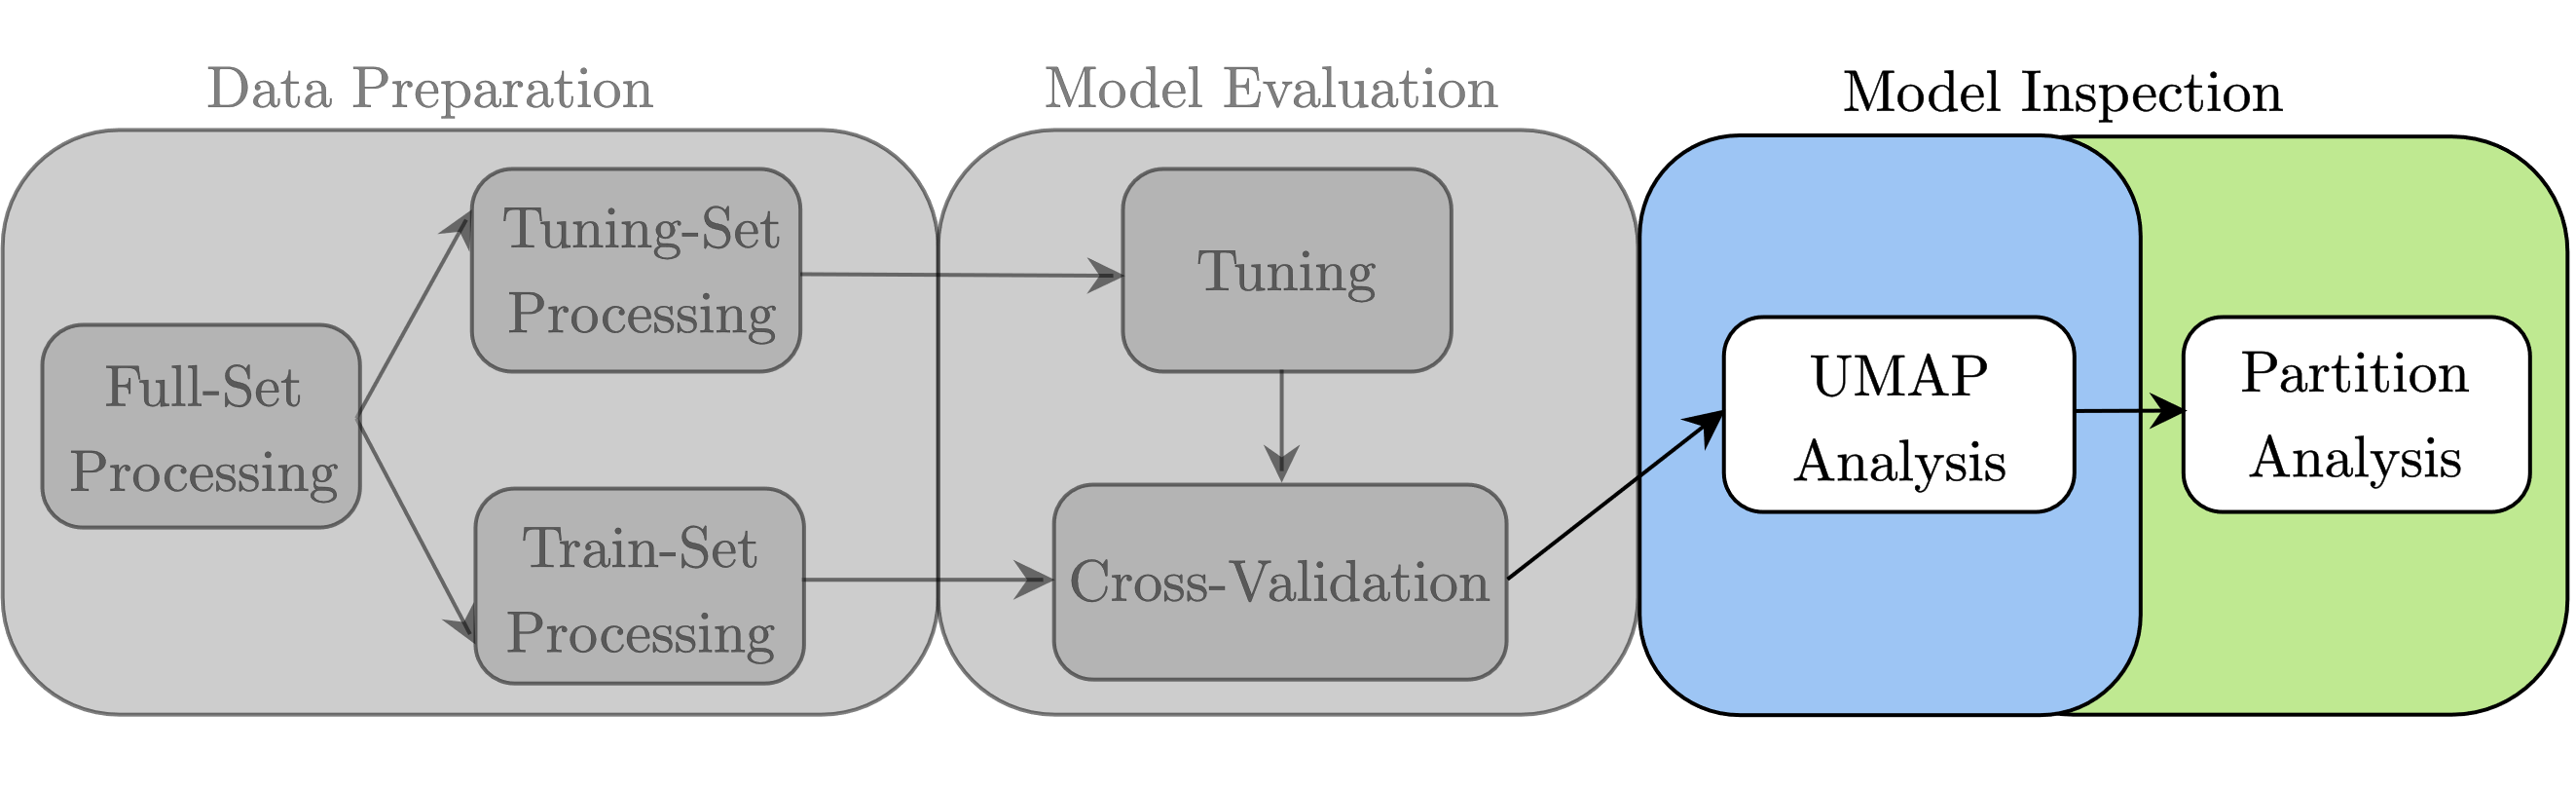
\includegraphics[width=\textwidth]{images/chapter_4/pipeline_inspect.png}
    \caption[\textbf{Representation analysis experimental pipeline}]{Arrows indicate the flow of the pipeline. Big coloured blocks are major pipeline steps, white rectangles indicate sub-tasks within each step. This experimental pipeline stems directly from the "Model Evaluation" stage outline in figure \ref{fig: pipeline_eval}.}
    \label{fig: pipeline_inspect}
\end{figure}

\section{Extracting and Visualizing the Latent Representation}
\label{extract_visulize}

\subsection{Neural Networks, manifolds and embeddings}
\label{manifold_learning_embed}
As we mentioned in section \ref{chapter_theory_modelling}, ANNs approximate a function by mapping the input they receive to a lower dimensional manifold. By moving along this manifold it is possible to reach inputs with different characteristics and observe how they relate with the output produced by the model.

Despite the fact that the manifold structure learned by the model might be intrinsically low dimensional, it is usually stored (or better, it is "embedded"), in a (potentially sparse) high dimensional representation \cite{bengio2017deep}. This representation usually has fewer degrees of freedom than the original input but it is still challenging to parse from a human perspective. Simplifying, this can be compared to storing the "instructions" on how to extract the low dimensional manifold from the input in a distributed fashion across all the parameters of the ANNs. In our case if we look at Figures \ref{fig: rnn_2} and \ref{fig: rnn_env_even}, the portion of the architecture marked in red should, once fitted to the input data, provide us with the relevant "instructions" on how to obtain an approximation of the manifold structure describing the level of attributed incentive salience (see chapter \ref{chapter_theory_modelling} for the theoretical reasons behind this assertion).

As illustrated in sections \ref{artificial_neural_networks} and \ref{manifold_learning}, since an ANNs can be thought as directed acyclic computational graphs (DAGs), to obtain the representation produced at any point of a specific architecture it is sufficient to pass a given input through all the operations performed before that point. Figure \ref{fig: repr_extr} illustrate the process for the RNN architecture presented in section \ref{model_architecture_2}.

\begin{figure}[!htb]
  \centering
  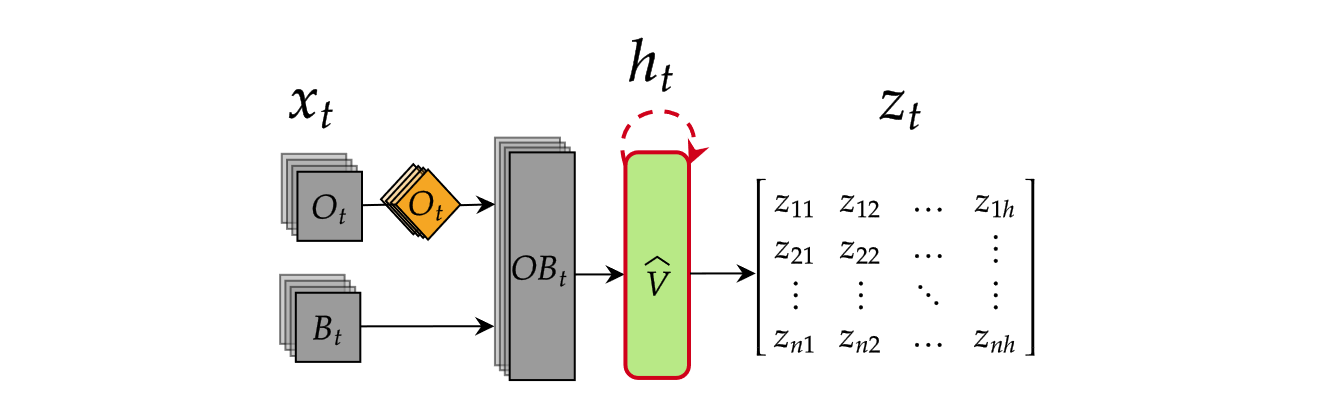
\includegraphics[width=\textwidth]{images/chapter_4/representation_extractor.png}
    \caption[\textbf{The procedure for generating latent representations generated by an ANN}]{Orange and green shapes represent respectively embedding and LSTM layers. Embedding layers are a type of feedforward layers specifically designed for dealing with categorical inputs \cite{chollet2015keras}. Gray shapes indicate operations with no learnable parameters, such as tensor instantiation and concatenation. The orange transparent shape indicate the concatenation of a single embedding with multiple tensors. Stacked, transparent colouring indicates arrays with a sequential structure. Straight and curved arrows refer to the presence of feed-forward or recurrent information flow. The red highlight shows the portion of the model that we hypothesize to be inferring an approximation of attributed incentive salience. Given inputs $O \in \mathbb{Z}^{N \times t}$ and $B \in \mathbb{R}^{N \times t \time 5}$, the matrix $Z_t \in \mathbb{R}^{N \times h}$ represents the $h$ dimensional (where $h$ is the number of hidden units in the recurrent layer) representation generated by the ANN at time $t$ after all operations in its underlying computational graph have been performed.}
    \label{fig: repr_extr}
\end{figure}

Borrowing the terminology from the self-supervised deep learning literature \cite{bengio2017deep} we call this truncated version of the original architecture encoder. Encoders can be thought as functions (whose parameters have been learned during the fitting procedure) mapping input data onto the manifold space learned by the original architecture. From now on, we will use the term encoder for referring to the two considered architectures truncated at the point of the last shared recurrent operation.

\subsection{Dimensionality Reduction and Manifold Approximation}
\label{dim_reduction}
If we look at figure \ref{fig: repr_extr} we can see that with as the size of $h$ increases, it becomes more and more challenging to inspect the representation generated by the encoder. However we recall from section \ref{manifold_learning_embed} that the intrinsic dimensionality for this representation should be much smaller. In the case of a latent state like attributed incentive salience this could be as small as one dimensional, or two if we consider the nature of the rewarding object (see section \ref{motivation_hist} and Figure \ref{fig: vect_mot} in particular). 

A convenient approach for inspecting the shape of this learned manifold would be to peform some form of dimensionality reduction. Principal Component Analysis (PCA) \cite{pearson1901liii} would be a reasonable approach given the straightforward interpretation of the derived components. However the choice of which algorithm to chose is not necessarily that straightforward. 

Looking at figure \ref{fig: swiss_ambient}, we can see the example of a dataset constituted by three separate (the separation aspect is important and will be further in section \ref{functional_properties}) point clouds (denoted by different colours) in a three dimensional ambient space (the space in which a low dimensional manifold might be embedded). Red and green clouds are examples of the synthetic Swiss Roll dataset \cite{scikit-learn}, while the blue cloud is a simple random projection of a square. Both datasets are basically equivalent (i.e. intrinsically two dimensional with the main dimension highlighted by the colour gradient) but differ in their layout in ambient space: the square is linear while the Swiss roll warps in a non linear fashion.

\begin{figure}[!htb]
  \centering
  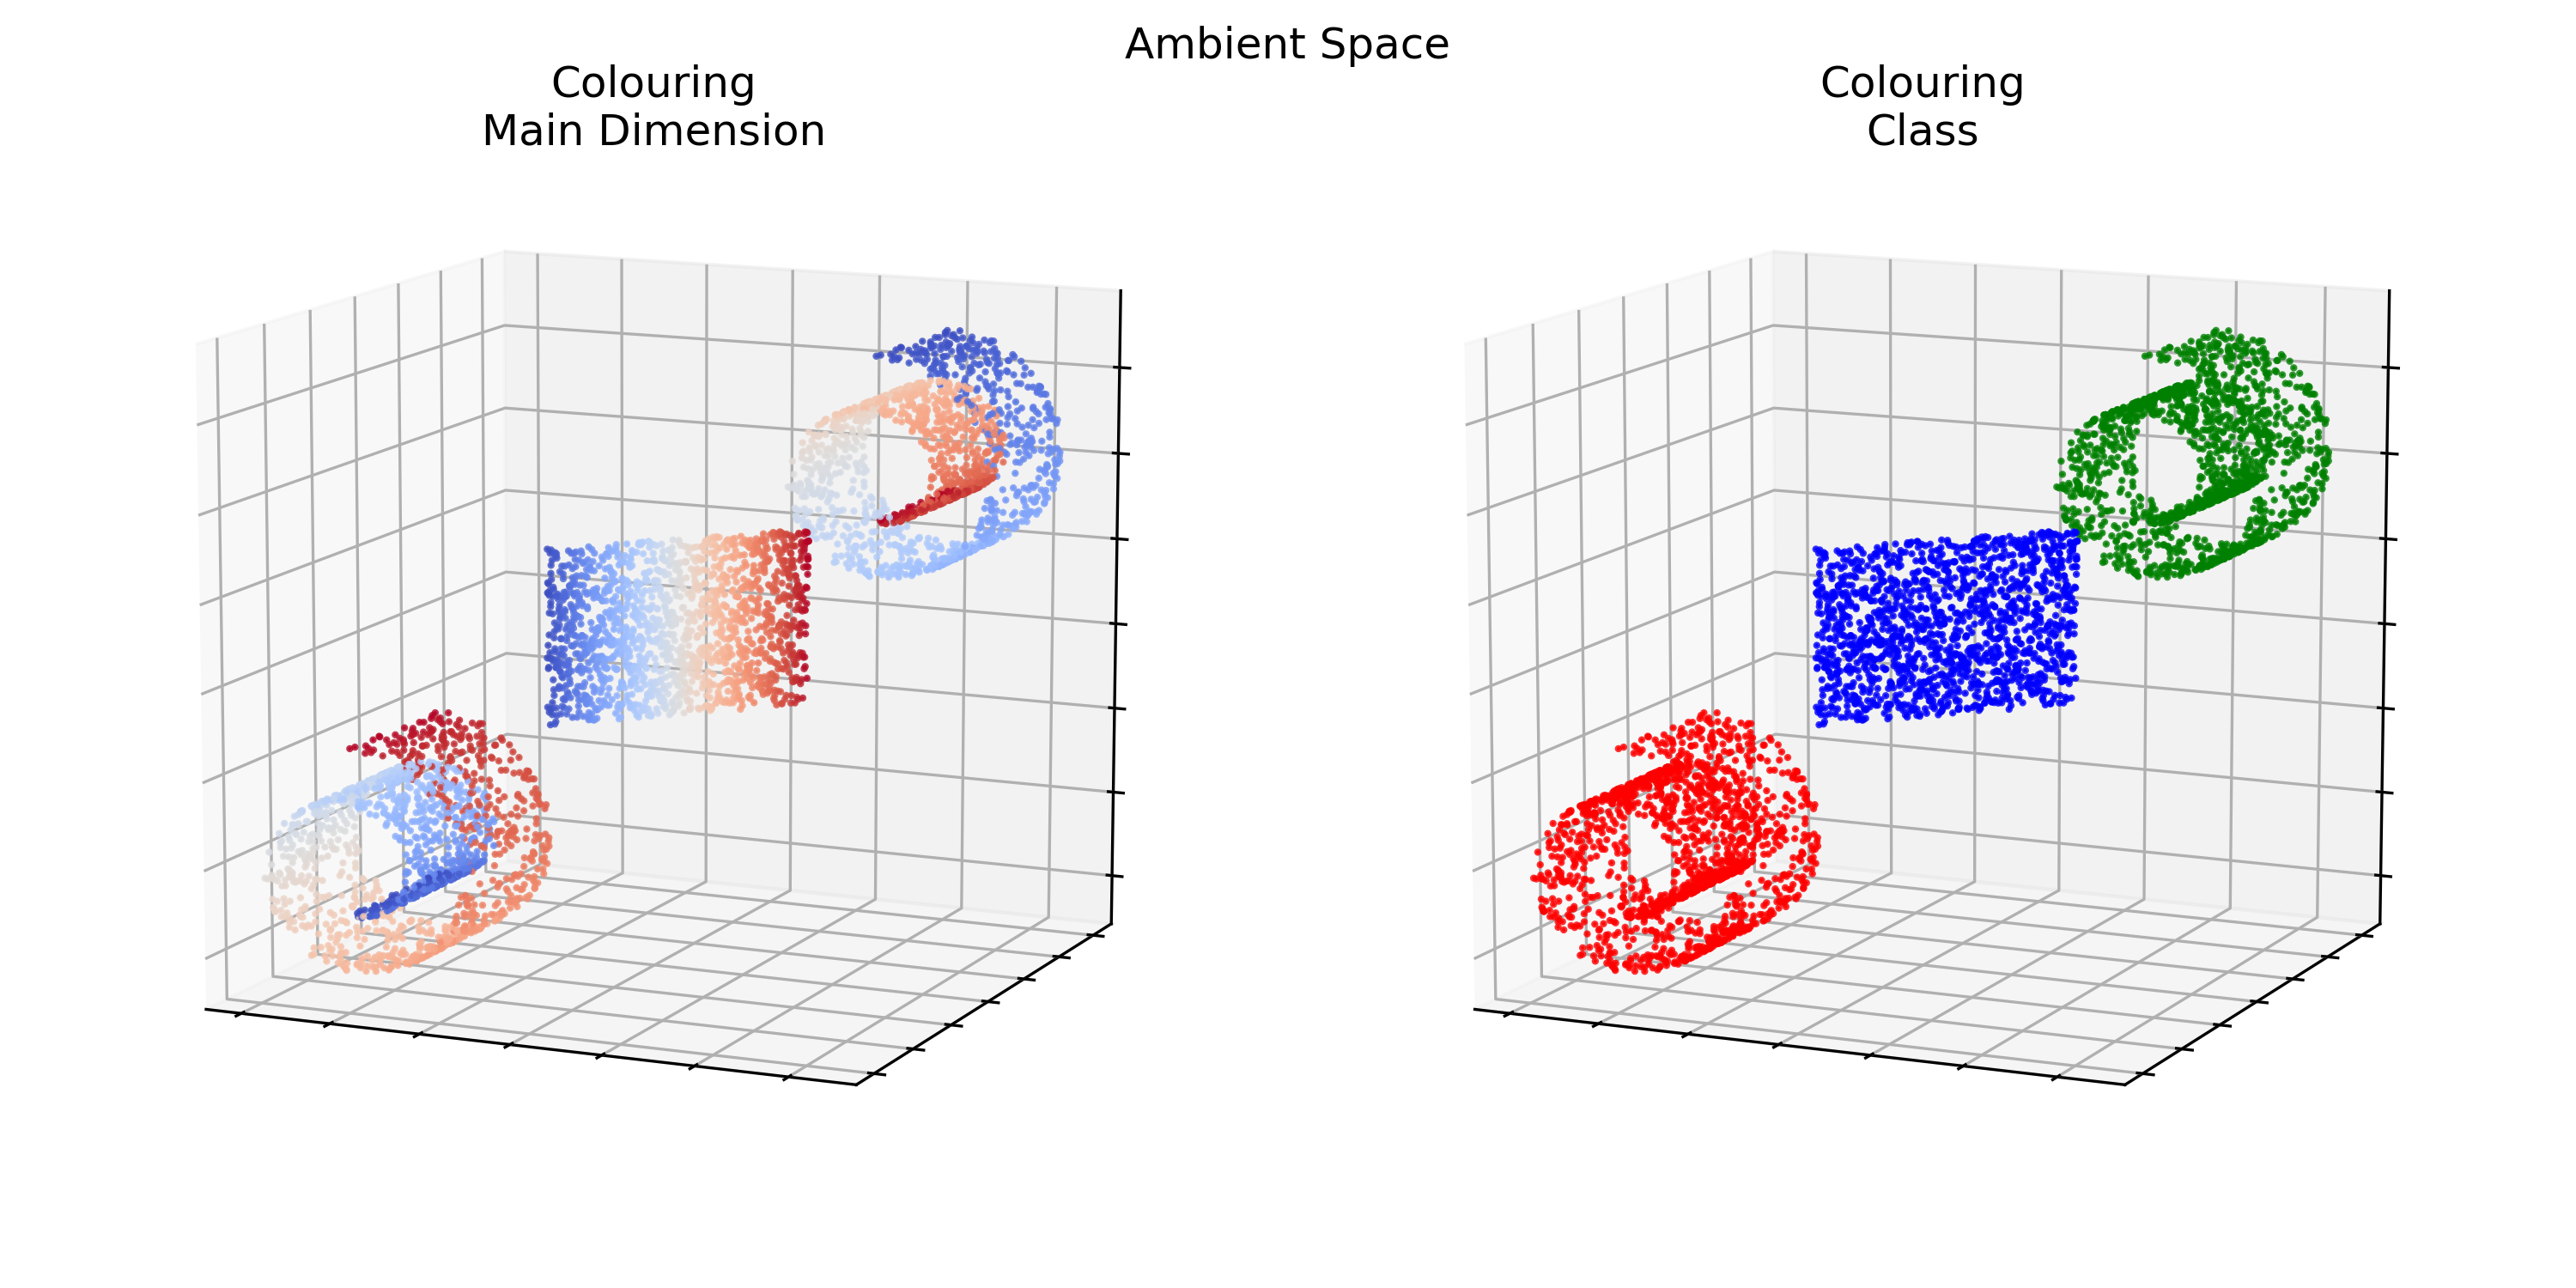
\includegraphics[width=\textwidth]{images/chapter_4/ambient.png}
    \caption[\textbf{Swiss rolls and square in ambient space}]{The figure shows three point clouds which are intrinsically two-dimensional (a Swiss roll and a square) embedded in a three-dimensional ambient space. In both panels the X, y and z axes represent the coordinates of the ambient space. The colours in the first panel indicates the main dimension of variation while those in the second panel simply identify membership of points to a specific cloud.}
    \label{fig: swiss_ambient}
\end{figure}

Figure \ref{fig: swiss_reduce} shows a dimensionality reduction performed by PCA along with an alternative non-linear dimensionality reduction approach: the Uniform Manifold Approximation and Projection (UMAP) \cite{2018arXivUMAP}. 

\begin{figure}[!htb]
  \centering
  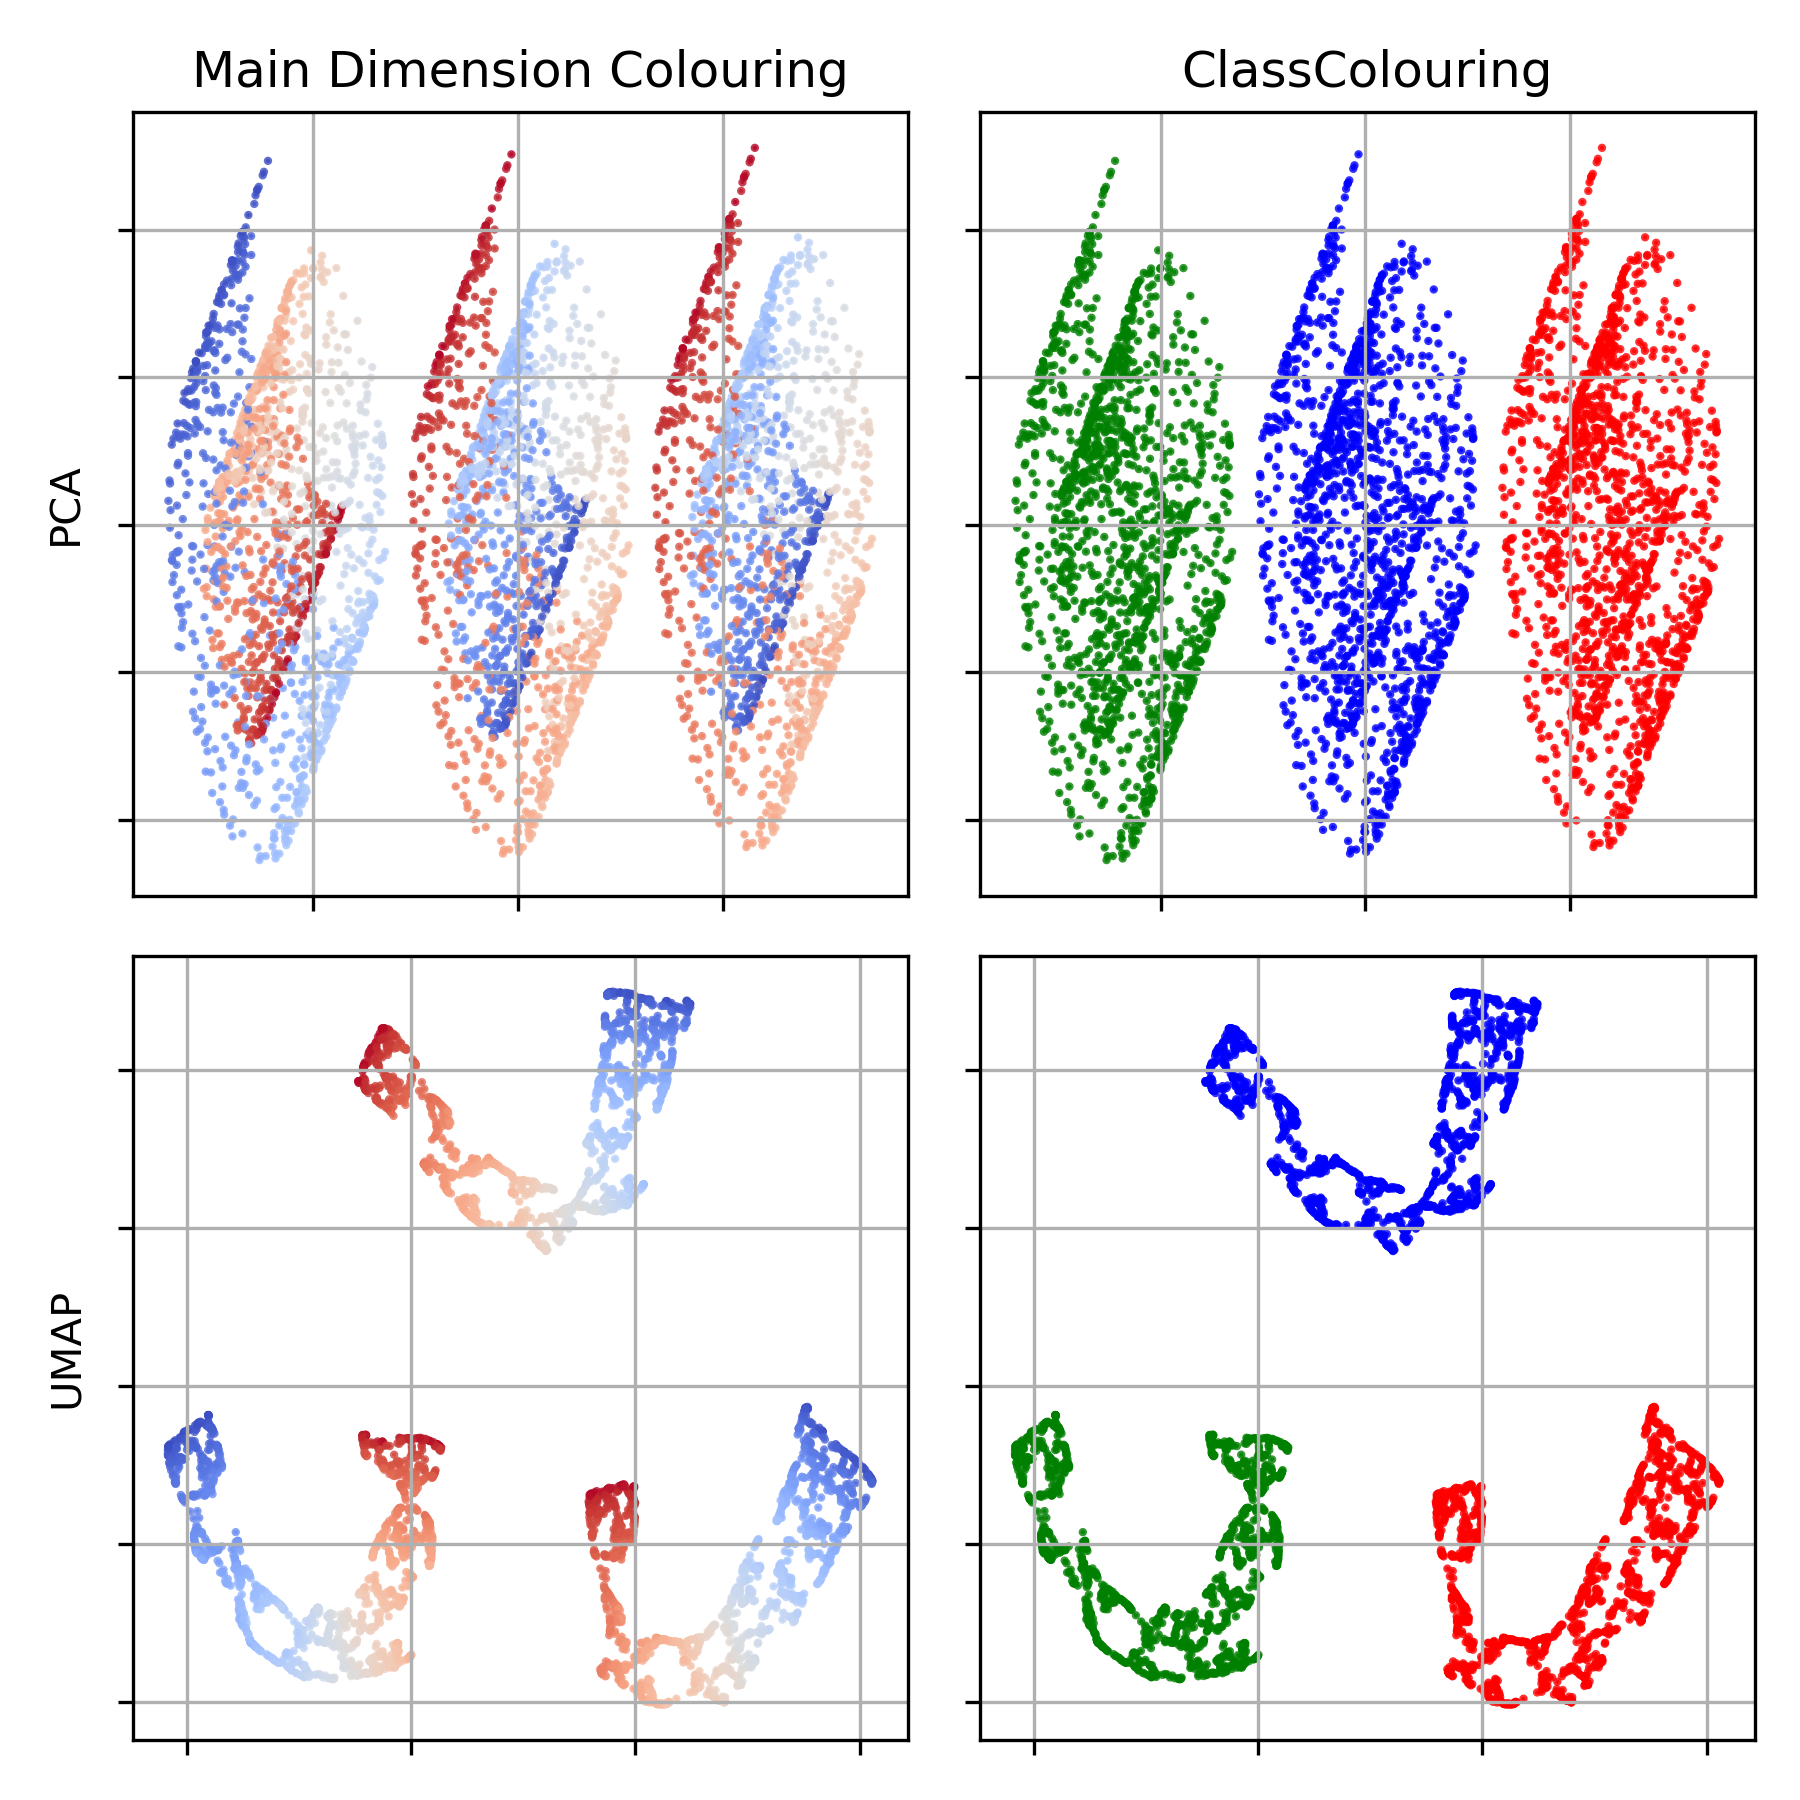
\includegraphics[width=0.7\textwidth]{images/chapter_4/reduced.png}
    \caption[\textbf{PCA and UMAP reduction of Swiss roll and square}]{The figure show the reduction of the three-dimensional point clouds to a two-dimensional plane. The panels in the first row show the reduction produced by PCA while those in the second row show the reduction produced by UMAP. In all panels the x, y axes represent the components extracted by PCA and UMAP. The colours in the two columns again indicate the main dimension of variation and the membership of points to a specific cloud.}
    \label{fig: swiss_reduce}
\end{figure}

The UMAP algorithm is a dimensionality reduction technique based on manifold learning. Given a high dimensional dataset, UMAP first infers its topological structure by means of a k-nearest neighbours graph and then, using stochastic gradient descent, attempts to structurally reproduce it in a lower dimensional space (two or three for visualization purposes) \cite{2018arXivUMAP}. Despite being a local algorithm, compared to other similar approaches (for example, the t-distributed Stochastic Neighbor Embedding \cite{van2008visualizing}),  UMAP has the ability to better preserve the global structure of the original data. Moreover, when given datasets that are sequential in natures (like those produce by the recurrent part of our architecture) UMAP is able to include this characteristics during the optimization process \footnote{See \cite{alignedumap} for implementation details.} generating lower dimensional representations that are aligned over time. 

What we observe in Figure  \ref{fig: swiss_reduce} is that both techniques manage to keep the separation between point clouds, but that PCA, unlike  UMAP, struggles to faithfully represent the the intrinsic structure of the data. This toy example is particularly relevant in our case as the representations generated by ANNs are, by design, highly non-linear. This will be made evident in the next section where we will proceed at visualizing the representation learned by our ANNs architecture.

\section{Representation Analysis}
\label{representation_analysis}
In order to support our idea that the representation learned by the different architectures could be interpreted as an approximation of the latent states generated by incentive salience, we carried out a series of qualitative analyses. If our intuitions were in the right direction, we expected the representations inferred by the architectures to exhibit a series of characteristics and functional properties:
\begin{enumerate}
    \item To possess an intrinsic dimensionality that is much smaller than the observed one.
    \item To be able to effectively distinguish between different game objects.
    \item To be able to effectively distinguish between individuals based on the expected intensity of their future interactions with the considered game objects.
    \item To be able to show the two aforementioned characteristics consistently over time.
\end{enumerate}

The characteristics mentioned above are concerned with a general validation of the properties of the latent representation for all the considered architectures, however we also wanted to understand if the included covariates altered and improved the generated representation.  We therefore inspected the representation extracted by the encoder derived from the improved version of the RNN architecture. 

The procedure followed for extracting the latent representations was the same for all architectures. First, we re-fitted all models on a random sample (i.e. 90\%) of the validation-set following the same procedures specified in chapter \ref{chapter_implementation_testing}. Then, we created six encoders using the approach illustrated in paragraph \ref{manifold_learning_embed} and Figure \ref{fig: repr_extr}. Two were used for extracting the representations expected to approximate the level of attributed incentive salience (red highlights in Figures \ref{fig: rnn_2} and \ref{fig: rnn_env_even}. One for extracting the same type of representation inferred however by the MLP architecture (this was done for comparative purposes). And three were used for extracting the intermediate representations generated by the improved version of the RNN architecture (i.e. those relative to the behavioural, environmental and game events input). Subsequently, we passed the remaining portion of the validation-set (i.e. 10\%) as an input to the encoders, producing arrays of shape $(N \times T \times h)$ with $N$ being the number of considered individuals, $h$ the number of hidden units in the last layer of the encoder and $T$ the number of observed interactions for the considered individuals. This means that all representations have been generated with out-of-sample data. In our case, since all architectures were of type sequence-to-sequence we were able to investigate not just the properties of the generated representation at specific point in time, but also the dynamics underlying their evolution. 

To summarize, each considered encoder was tasked with generating a high dimensional representation where distance could be interpreted as similarity between individuals with respect to the expected intensity of their future interactions with a specific game object (see the manifold hypothesis of attributed incentive salience presented in paragraph \ref{manifold_rep_incentive_salience}). Dimensionality reduction was then used for approximating the intrinsic manifold structure of these representations on a two dimensional plane in order to allow for qualitative visual analysis. 

The reduction to a 2D plane used the UMAP algorithm. The algorithm first inferred the topological structure of the produced representations by computing the cosine distance in a local neighborhood of 1000 points with a minimum distance of 0.8. The projection on a two dimensional plane was then achieved by running the optimization part of the algorithm for 2000 iterations. The choice of a large neighborhood and minimum distance was made to better capture the global structure of the manifold \footnote{See \cite{umapwebs} for a visualization of the effects of these hyperparameters in UMAP.}. 

In order to gather an understanding on the characteristics of the function used for generating the latent representations, we also conducted a set of purely exploratory investigations of the relationship between hidden units' activation in the recurrent layers and the predictions produced by the model. To quantify the strength of the observed relationship we employed the Maximal Information Coefficient (MIC) \cite{reshef2011detecting}, a measure of mutual information that can quantify both linear and non-linear association between variables. The MIC can assume values between 0 to 1 with 1 corresponding to a perfect association. 

We adopted the implementation of UMAP provided McInnes \textit{et. al.} \cite{mcinnes2018umap-software} while the MIC was computed using the python library minepy \cite{albanese2013minerva}. Visualizations were produced using the python libraries matplotlib \cite{hunter2007matplotlib} and seaborn \cite{waskom2021seaborn}.

\subsection{Validating the Functional Properties of the Inferred Latent Representation}
\label{functional_properties}
We first asked if the assumption about the intrinsic dimensionality of the latent representation was reasonable. Looking at figure \ref{cross_corr_act}

\begin{figure}[!htb]
\centering
\includegraphics[width=0.5\textwidth]{images/chapter_4/corr_matrices.png}
\caption[\textbf{Cross-correlation analysis of the hidden units activation of the RNN architecture}]{Each panel shows the cross correlation between the activity of the RNN's artificial neurons in all the game objects going from $t1$ to $t4$. The y and x axes are symmetrical and identify the RNN artificial neurons while the coloured cells indicate the Spearman's Rho correlation coefficient for the activation of each pair of neurons. White cells represent combinations for which the correlation coefficient was lower than 0.05.}
\label{cross_corr_act} 
\end{figure}

we can observe consistent patterns of cross-correlation for the activity of the hidden units constituting the latent representation, suggesting the presence of redundancy. In order to support this finding and to gain a general sense of the intrinsic dimensionality of the embedded manifold, we conducted a Principal Component Analysis (PCA). Despite PCA and UMAP working under radically different assumptions and mechanisms, we thought this could provide us with a general idea of how much variance we would be able to capture by reducing the representation to a lower dimensional space. 

\begin{figure}[!htb]
\centering
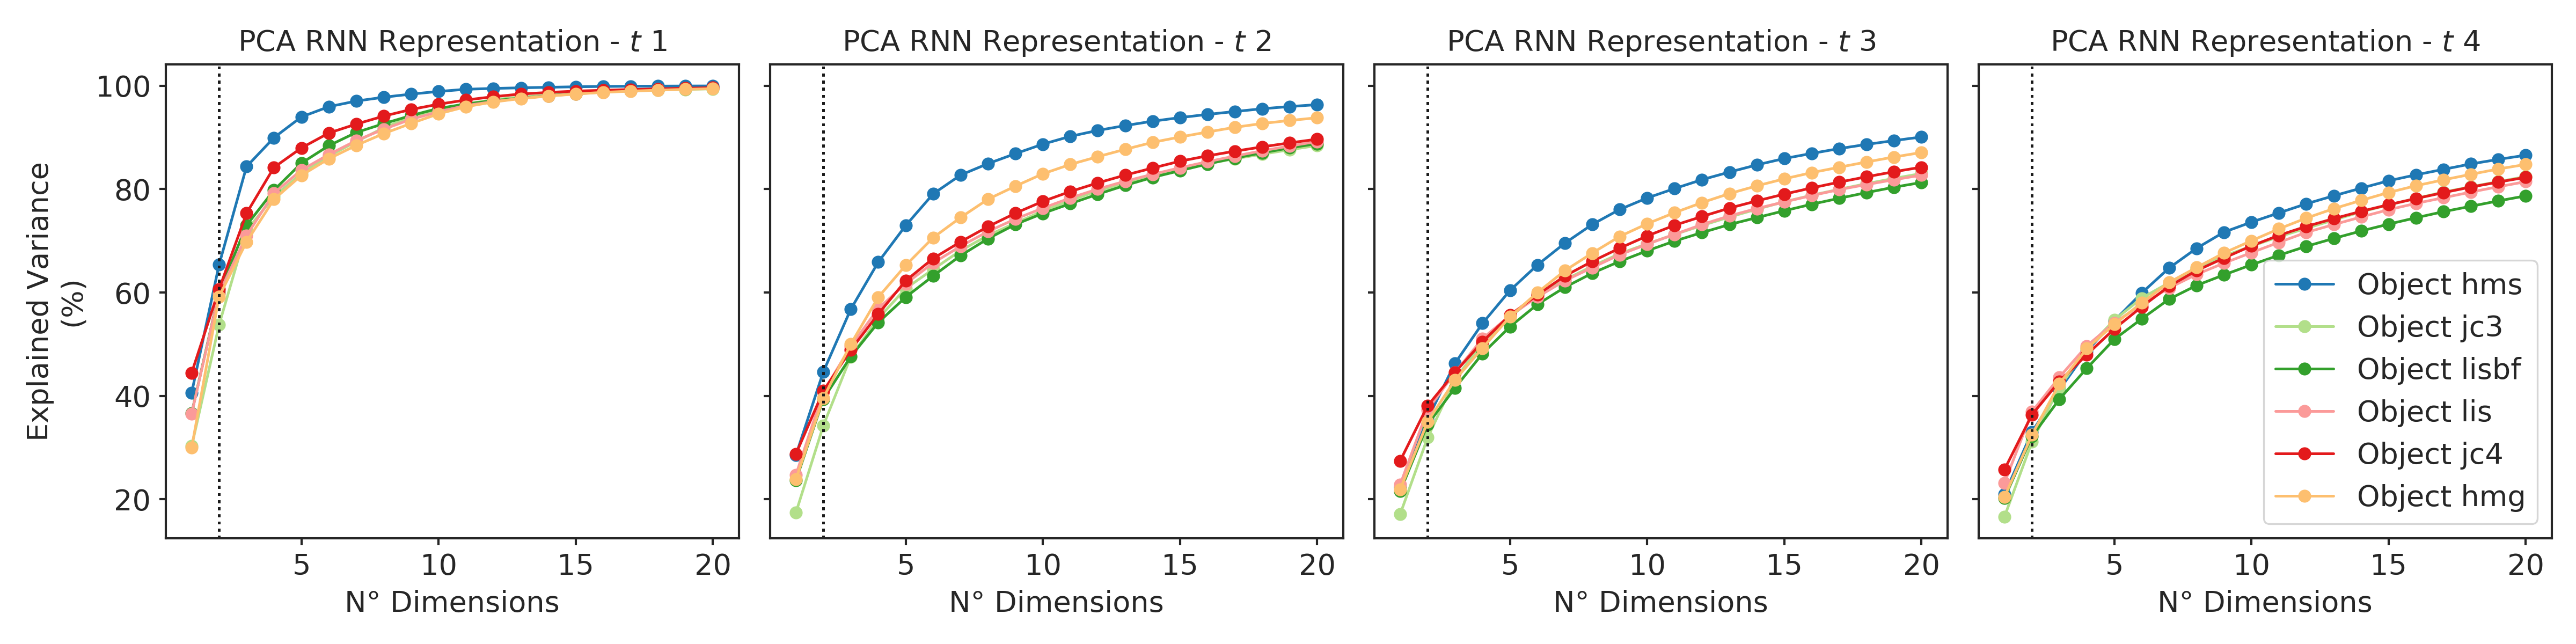
\includegraphics[width=\textwidth]{images/chapter_4/pca_embedding.png}
\caption[\textbf{Principal component analysis of the hidden units activation of the RNN architecture }]{The panel shows the percentage of explained variance by considering 2 to 20 principal components for each game object going from $t1$ to $t4$. The y axis indicates the percentage of explained variance while the x axis the number of principal components considered.}
\label{pca_emb} 
\end{figure}

Looking at figure \ref{pca_emb} we can see that two principal components can explain a large portion of variance in the representation generated by the RNN. To be precise, across game contexts the first two principal components were able to explain from 30 to 60\% of the variance, with maximum explanatory power around 6 and 8 principal components. However, as we illustrated in section \ref{dim_reduction}, relying on PCA alone could give us an incomplete and potentially distorted picture of the manifold structure inferred by the architecture. Looking at Figure \ref{temporal_panel_rnn_pca} 

\begin{figure}[!htb]
\centering
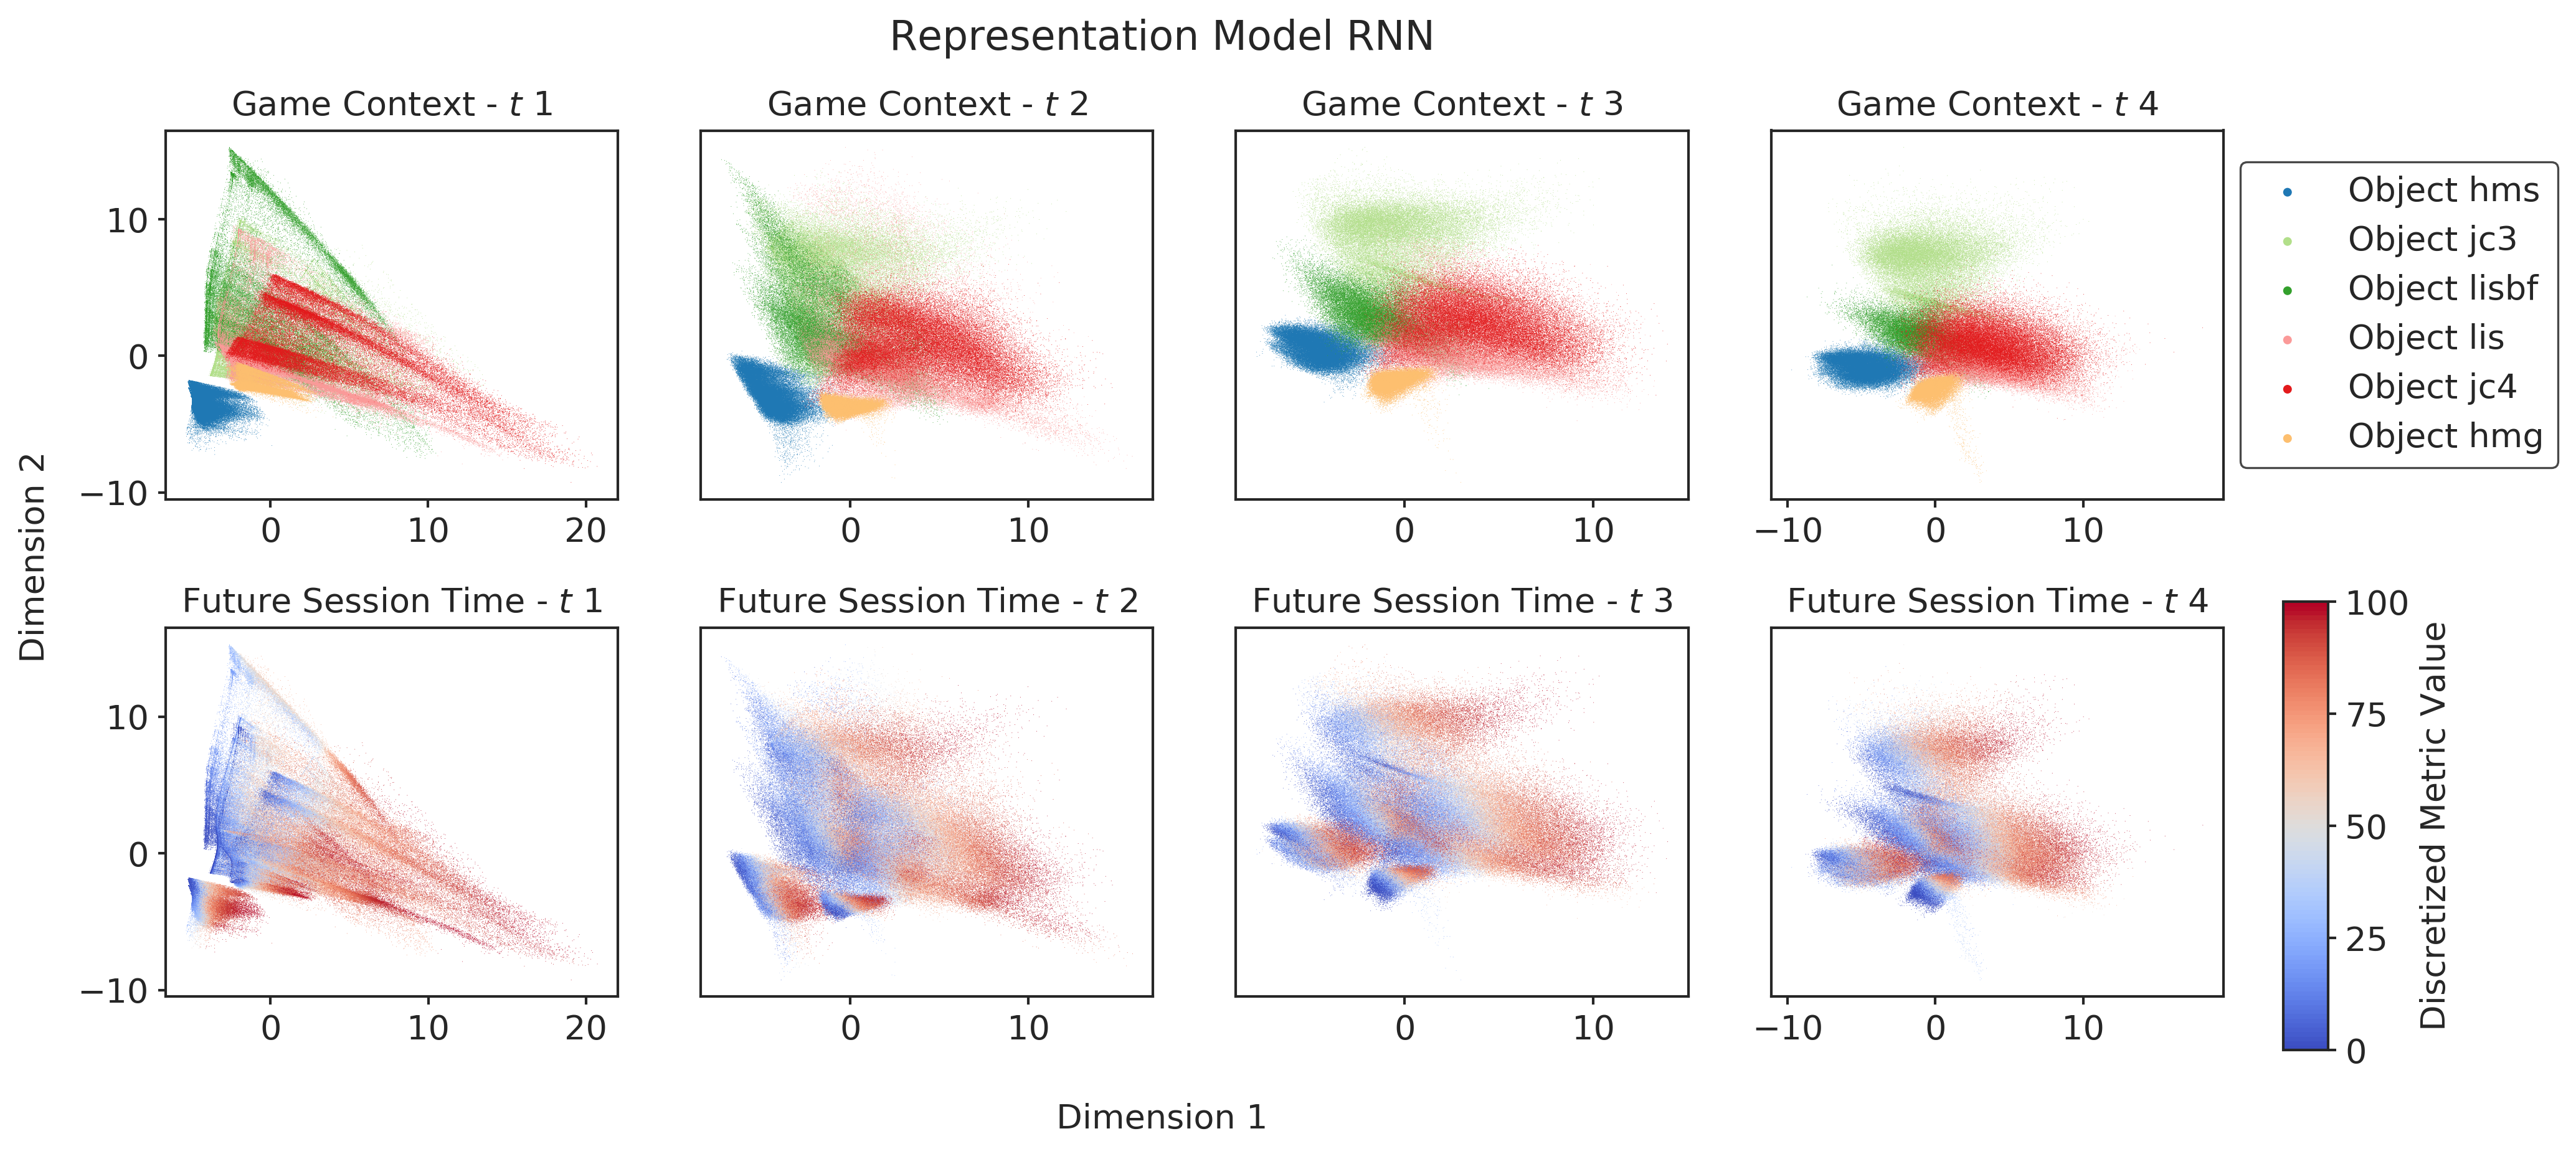
\includegraphics[width=\textwidth]{images/chapter_4/rnn_future_sess_pca.png}
\caption[\textbf{Lower dimensional representation of the latent state generated by the RNN architecture using PCA}]{The figure shows the two-dimensional projection, produced by PCA, of the multi-dimensional representation inferred by the RNN for interactions going from $t1$ to $t4$. We can read the values of the x and y axes as the first two directions of maximum variation in the latent representation. Each point indicates the representation inferred by the RNN model after observing one game session from a single user. The colours in the first row indicate the game object from which the representation is coming. Colours in the second row represent the discounted sum of all future predictions for a particular target (for example, estimated Future Session Time) $\widehat{B}_{t2:T}$ which is given by $\sum_{i=0}^{t2:T} \gamma^i\widehat{B_i}$ with $\gamma=0.1$ as illustrated in the TD Learning equation \ref{td_v}}
\label{temporal_panel_rnn_pca}
\end{figure}

we can see that the representation seems to embed a single gradient line that distinguishes individuals based on the expected length of their future interactions (here future session time) with the considered game objects. However, the low dimensional projection appears to be organized in a disorderly manner, with game contexts blending into each other causing the gradient line to look discontinuous. 

The projection produced by the UMAP algorithm, on the other side, appears to provide a better picture of the inherent structure of the inferred representation. Looking at Figure \ref{full_panel_static}A 

\begin{figure}[!htb]
\centering
\includegraphics[width=\textwidth]{images/chapter_4/static_repr_42.png}
\caption[\textbf{Lower dimensional representation of the latent state generated by the RNN architecture}]{The representation generated by the RNN model distinguishes between different game objects while maintaining an overarching organization able to capture variations in the expected intensity of future interactions that individuals will have with a specific game object. Panel A shows the two-dimensional projection, produced by UMAP, of the multi-dimensional representation inferred by the RNN at $\mathbf{t1}$ as produced by UMAP. We can read the values of the x and y axes as a coordinate system where proximity represents similarity between points in the original high-dimensional space. Each point indicates the representation inferred by the RNN model after observing one game session from a single user. The colours in the Game Context panel indicate the game object from which the representation is coming. Colours in the small panels represent the discounted sum of all future predictions for a particular target (for example, estimated Future Session Time) $\widehat{B}_{t2:T}$ which is given by $\sum_{i=0}^{t2:T} \gamma^i\widehat{B_i}$ with $\gamma=0.1$ as illustrated in equation \ref{td_v}. Each unit  encodes the intensity of future interactions through multiple non-monotonic functions. Panels B and C show the relationship between the activation of randomly-selected hidden units in the LSTM layer of the RNN and the model's predictions at $\mathbf{t1}$. Panel B shows the relationship between the discretized activation of 10 randomly selected units (artificial neurons) plotted along the y axis and the predictions made by the model at $t1$ (colour coded from blue to red as in the small panels in A) for the game object $hmg$. Panel C shows in more detail the relationship between discretized activation and RNN predictions for a single unit highlighted by a black box in Panel B. Here the x axis indicates the discretized activation while the y axis the mean discretized discounted sum of all future predictions produced by the model. Vertical lines are standard errors of the mean. The red curve is the line of best fit provided by a generalized additive model \cite{serven2018} while the box reports the MIC and the correlation coefficient (Spearman's $\rho$) between the artificial neuron activation and the model's predictions.}
\label{full_panel_static}
\end{figure}

we observe how the model was able to effectively distinguish between different game objects while simultaneously encoding for variations in the expected intensity of future interactions. This is illustrated by the fact that each game object occupies different and distinct regions in the representation space while showing a within-object gradient-like organization that places individuals (i.e. single dots) on a continuum based on the estimated magnitude of their future behaviour. 

This organization is preserved for each of the six targets showing how the representation inferred by the model is a suitable meta-descriptor for different behavioural indicators. As expected, some targets show a very similar but not identical organization (e.g. Future Session Time and Future Session Activity) while others appear to be independent (e.g. Future Session Time and Future Absence). We note that the absolute location of each game aggregate (i.e. all the points belonging to a specific game object) on the 2D plane is arbitrary. 

Panels \ref{full_panel_static}B and \ref{full_panel_static}C provide more insight into the activation profiles of individual hidden units constituting the generated representation. Panel \ref{full_panel_static}B shows the relationship between the activity of 10 randomly-chosen units and the predictions generated for the five targets. These are essentially transducer functions illustrating how the estimate for a particular target varies (on average) as the output of a units increases or decreases. Each unit seems to encode for multiple non-monotonic functions, one for each of the considered targets. Differences in the shape of these functions reflect similarities between their associated targets. For example, the functions associated to two highly related targets like Future Session Time and Future Session Activity (see panel \ref{full_panel_static}A) appear to be very similar in shape (see panels \ref{full_panel_static}B and \ref{full_panel_static}C). Interestingly, although most units appear to encode for unique functions some of them (e.g. 41 and 44) show an almost identical behaviour. This suggests the presence of redundancy in the functions underlying the representation generated by the RNN model. These observations are clarified in panel \ref{full_panel_static}C, where the functions associated with a single unit (20, indicated by a dark box in \ref{full_panel_static}B) are presented. Here we observe a strong, non-linear relationship between the unit's activity and the estimated targets (see the high MIC values and the line of best fit). In addition, the between-targets variation in MIC values suggest how the chosen unit is not equally informative for all targets but rather shows specialized  behaviour.

\begin{figure}[!htb]
\centering
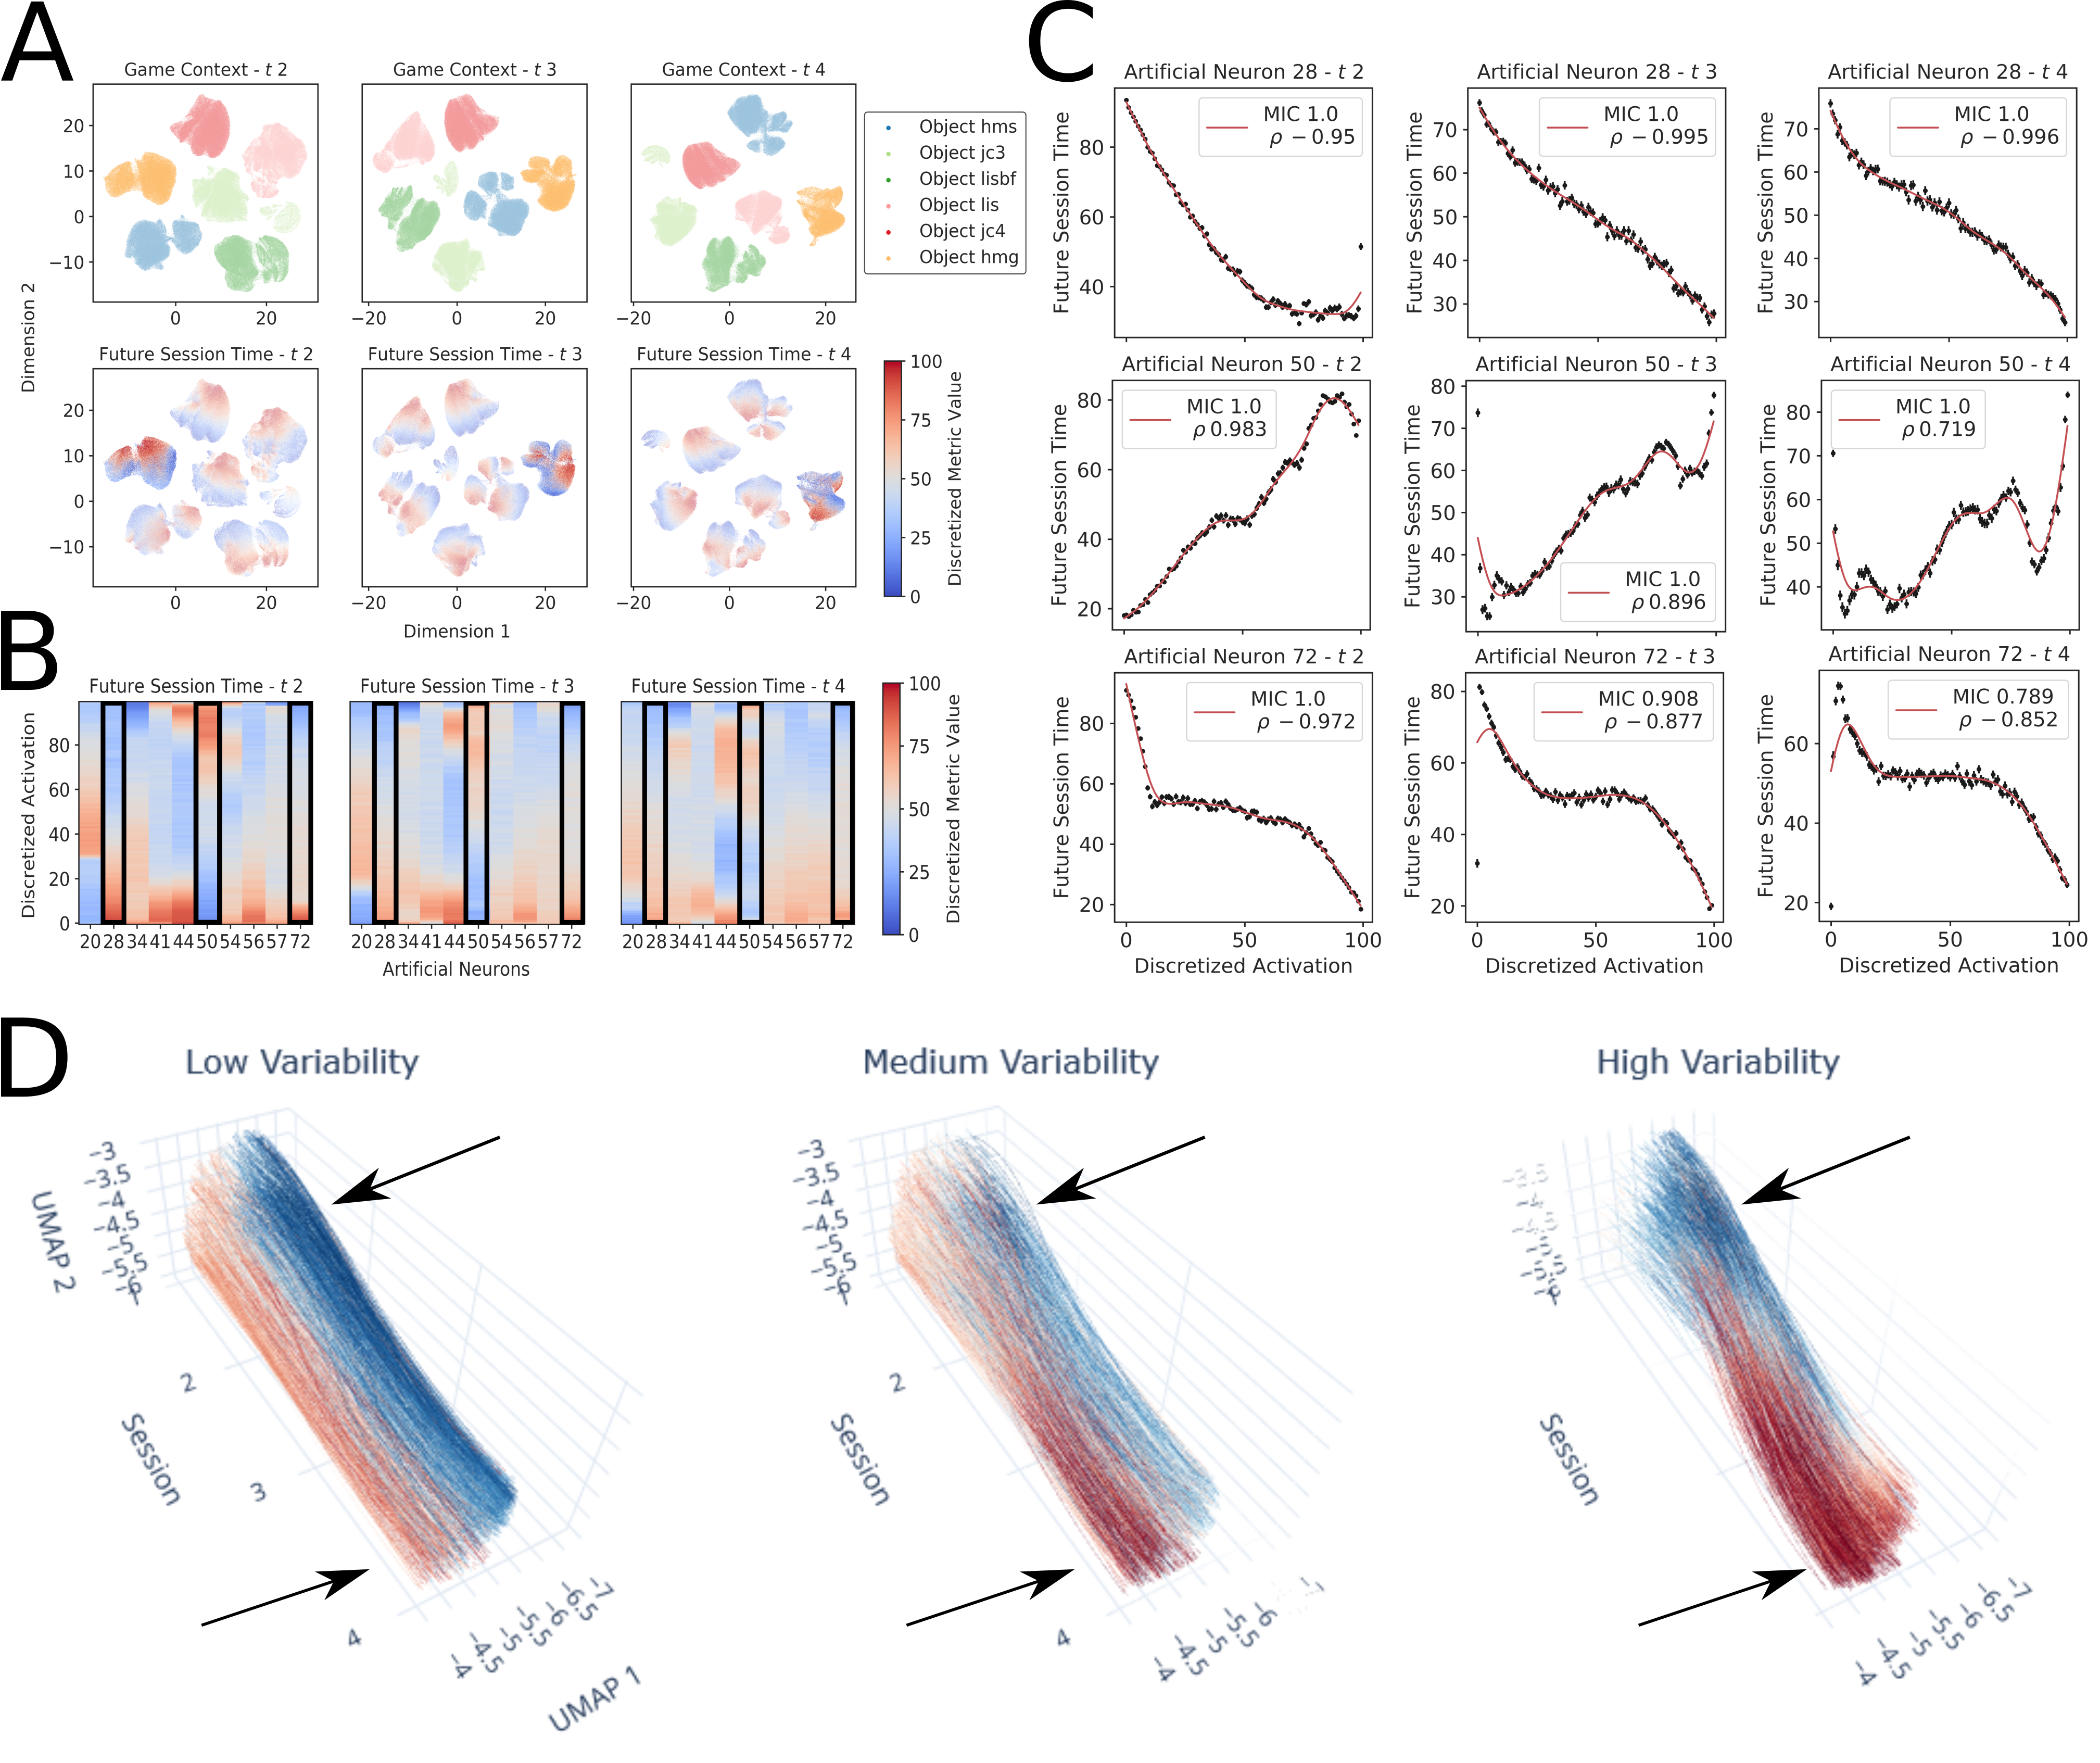
\includegraphics[width=\textwidth]{images/chapter_4/dynamic_repr_42.png}
\caption[\textbf{Lower dimensional representation of the evolution of the latent states generated by the RNN architecture}]{The representation generated by the RNN model appears to maintain its discriminant properties over time. Panel A shows a two-dimensional projection of the multi-dimensional representation inferred by the RNN at $t2$, $t3$ and $t4$. The inferred representation maintains its gradient-like organization over time with an increased ability to differentiate between game objects. As in Figure \ref{full_panel_static}, x and y axes are dimensions individuated by the UMAP algorithm and can be interpreted as a coordinate system where proximity represents similarity between points. Colours in the first row indicate which game object the representation is coming from while those in the second row indicate the discounted sum of future predictions for a single target (i.e. "Future Session Time"). \textbf{The units constituting the generated representation encode for functions that are consistent over time.} Panels B and C show the relationship between units' activation and the model's predictions over time for the game object $hmg$. Different units appear to encode the same target with different non non-monotonic functions which are relatively consistent over time. Panel B illustrates the relationship between the same 10 randomly selected units specified in figure \ref{full_panel_static} and the predictions made by the model for Future Session Time at $t2$, $t3$ and $t4$. Panel C shows in more detail the relationship of the three artificial neurons, highlighted by black boxes in B, across time. Each row is a different unit while each column corresponds to a different $t$. The x axis indicates the discretized activation while the y axis the mean discretized discounted sum of all future predictions. Vertical lines are standard errors of the mean. The red curve is the line of best fit provided by a generalized additive model \cite{serven2018} while the box report the MIC and the correlation coefficient (Spearman's $\rho$) between the artificial neuron activation and the model's predictions. \textbf{The generated representation produces areas of low and high expected intensity among which individuals move over time.} Panel D shows trajectories through time produced by a version of UMAP that incorporates temporal information. Data are drawn from random subsets of individuals having low, medium and high variability in their expected amount of future behaviour. The representation inferred by the RNN model produces "hot" (i.e. the left side) and "cold" (i.e. the right side) regions, representing high and low expected Future Session Time, that are spatially consistent over time. Individuals appear to either stay in the same region or to move between regions over time. Here each line represents variations in the representation generated by the RNN model for a single user over four temporal steps. Continuity is generated by means of cubic spline interpolation for the lines and by linear interpolation for the colours. The x and y axes are the dimensions individuated by the UMAP algorithm while the z axis indicates the associated point in time. Colours indicate the discounted sum of future predictions produced by the model at a specific point in time.}
\label{full_panel_temporal}
\end{figure}

The analyses in Figure \ref{full_panel_static} were performed at a single time point $t1$. However, as we mentioned before, the characteristics of our architectures allowed us to also evaluate how the latent representation evolved over time. 

Looking at Figure \ref{full_panel_temporal}, we can see that the characteristics detected at a single point in time remain qualitatively consistent over time. For example, focusing on Future Session Time (see Appendix \ref{rnn_architecture_representations} for results connected to other targets), we see in Figure \ref{full_panel_temporal}A that the model's ability to segregate different game objects while providing an  overarching representation of the intensity of future interactions is preserved over time. This supports the hypothesis that the representation inferred by our model is dynamic in nature which is further corroborated by panel \ref{full_panel_temporal}D. There we can see how the RNN model was able to individuate a "space" with temporally consistent ”hot” and ”cold” regions between which individuals gradually moved over time depending on the expected intensity of their future interactions. This means that given the history of interaction of a particular individual with a specific game object, our model would determine their "position" (i.e. their "internal state") in a latent space indicative of the expected intensity of future interactions with that object. If we recall our definition of attributed incentive salience from chapters \ref{chapter_lit_review} and \ref{chapter_theory_modelling} we can suggest that the model has inferred the location of individuals in what is an approximation (from the functional point of view) of the "attributed incentive salience space". This aligns with the manifold hypothesis mentioned in sections \ref{manifold_rep_incentive_salience} and \ref{manifold_learning}: changes in the propensity to interact with a specific game object (i.e. variations in the amount of attributed incentive salience) can be expressed moving on a manifold embedded within an $h$ dimensional space, with $h$ being the dimensionality of the representation generated by our RNN model. 

It appears that the hidden units constituting this representation tend to be consistent over time in the type of functions they encode (see Figure \ref{full_panel_temporal}B and C). As expected, we can again observe a strong non linear association between units' activation and targets' predictions, see MIC values and lines of best fit. The decrease in MIC value observed in Figure \ref{full_panel_temporal}C for the artificial neuron 72 might indicate how certain units lose their informative power over time.

\begin{figure}[!htb]
\centering
\includegraphics[width=\textwidth]{images/chapter_4/RNN_MLP_repr_42.png}
\caption[\textbf{Lower dimensional representation of the latent states generated by the time-distributed MLP architecture}]{The representation generated by the MLP model is less effective at distinguishing between different game objects and different levels of expected future behaviour intensity. Panel A shows a two-dimensional projection of the multi-dimensional representation inferred by the MLP at $t1$, $t2$, $t3$ and $t4$. Differently from the RNN, the representation shows a disruption in the gradient-like organization and a reduced ability to differentiate between game objects which remain constant over time. The x and y axes are dimensions individuated by the UMAP algorithm and can be interpreted as a coordinate system where proximity represents similarity between points. Colours in the first row indicate which game object the representation is coming from while those in the second row indicate the discounted sum of future predictions for a single target (i.e. "Future N° of Sessions") \textbf{The representation generated by the MLP model is less effective at at distinguishing different levels of expected behaviour intensity for states that are further away in the future.} Panel B shows a two-dimensional projection of the multi-dimensional representation inferred by the RNN (left) and MLP(right) at $t1$ but colour coded with the discounted sum of future predictions from $t4$ onward. The representation generated by the RNN is able to maintain a gradient-like organization even from states that are further away in the future while this capacity is almost entirely lost for the MLP. The colours in the Game Context panel indicate the game object from which the representation is coming. Colours in the small panels represent the discounted sum of all future predictions for a particular target computed from $t4$ onward instead that from $t1$. The x and y axes are the dimensions individuated by the UMAP algorithm.}
\label{predictive_panel}
\end{figure}

If we look at the differences between MLP and RNN-like architectures from section \ref{model_architecture_2}, we can see that they all aim to solve the same task: predict the intensity of future behaviour given the history of interactions. They do so relying on the same type of metrics, leveraging similar computational mechanisms (i.e. multitask learning and non-linearity) and producing representation according to the same underlying principle (i.e. the manifold hypothesis). Nevertheless, the fact that MLP architectures consistently provided poorer fit to data already suggests that whatever representation it had inferred it was likely a sub-optimal approximation of the manifold structure of attributed incentive salience. 

Looking at figure \ref{predictive_panel}A, and knowing that UMAP represents differences and similarities between points through distance, we can see how the representation generated by the MLP less clearly differentiate between game objects. On the same figure, we can notice how the gradient representation for the metric Future N° Sessions is largely disrupted. This effect is however consistently less pronounced for other metrics (see Appendix \ref{mlp_architecture_representations} for additional visualizations) and in accordance to the differences in predictive perfromance that we observed in chapter \ref{chapter_implementation_testing}. 

Recalling what mentioned in section \ref{comp_framework}, the latent state produced by the level of attributed incentive salience should retain at any point in time some predictive power over the intensity of all the future interactions (i.e. not just the one that follows). Figure \ref{predictive_panel}B shows the representation generated by RNN and MLP at $t1$ but color coded with the discounted sum of the predictions made from $t4$ onward. We can see that, even if degraded, RNN still preserves some of the desired gradient-like organization which is instead much more disrupted for MLP. This is in accordance to what is shown by Figure \ref{full_panel_temporal}D: the RNN appears to define regions of high and low expected behavioural intensity which are consistent over time rather than generating representations that are mostly representative of what is expected at $t+1$.

\subsection{Evaluating the Contribution of Environmental and Game Events Covariates}
\label{representation_env_even_contr}
Shifting our attention to the representations generated by the improved version of the RNN architecture we can see some noticeable differences. Looking at Figure \ref{rnn_env_even_full_beha} 

\begin{figure}[!htb]
\centering
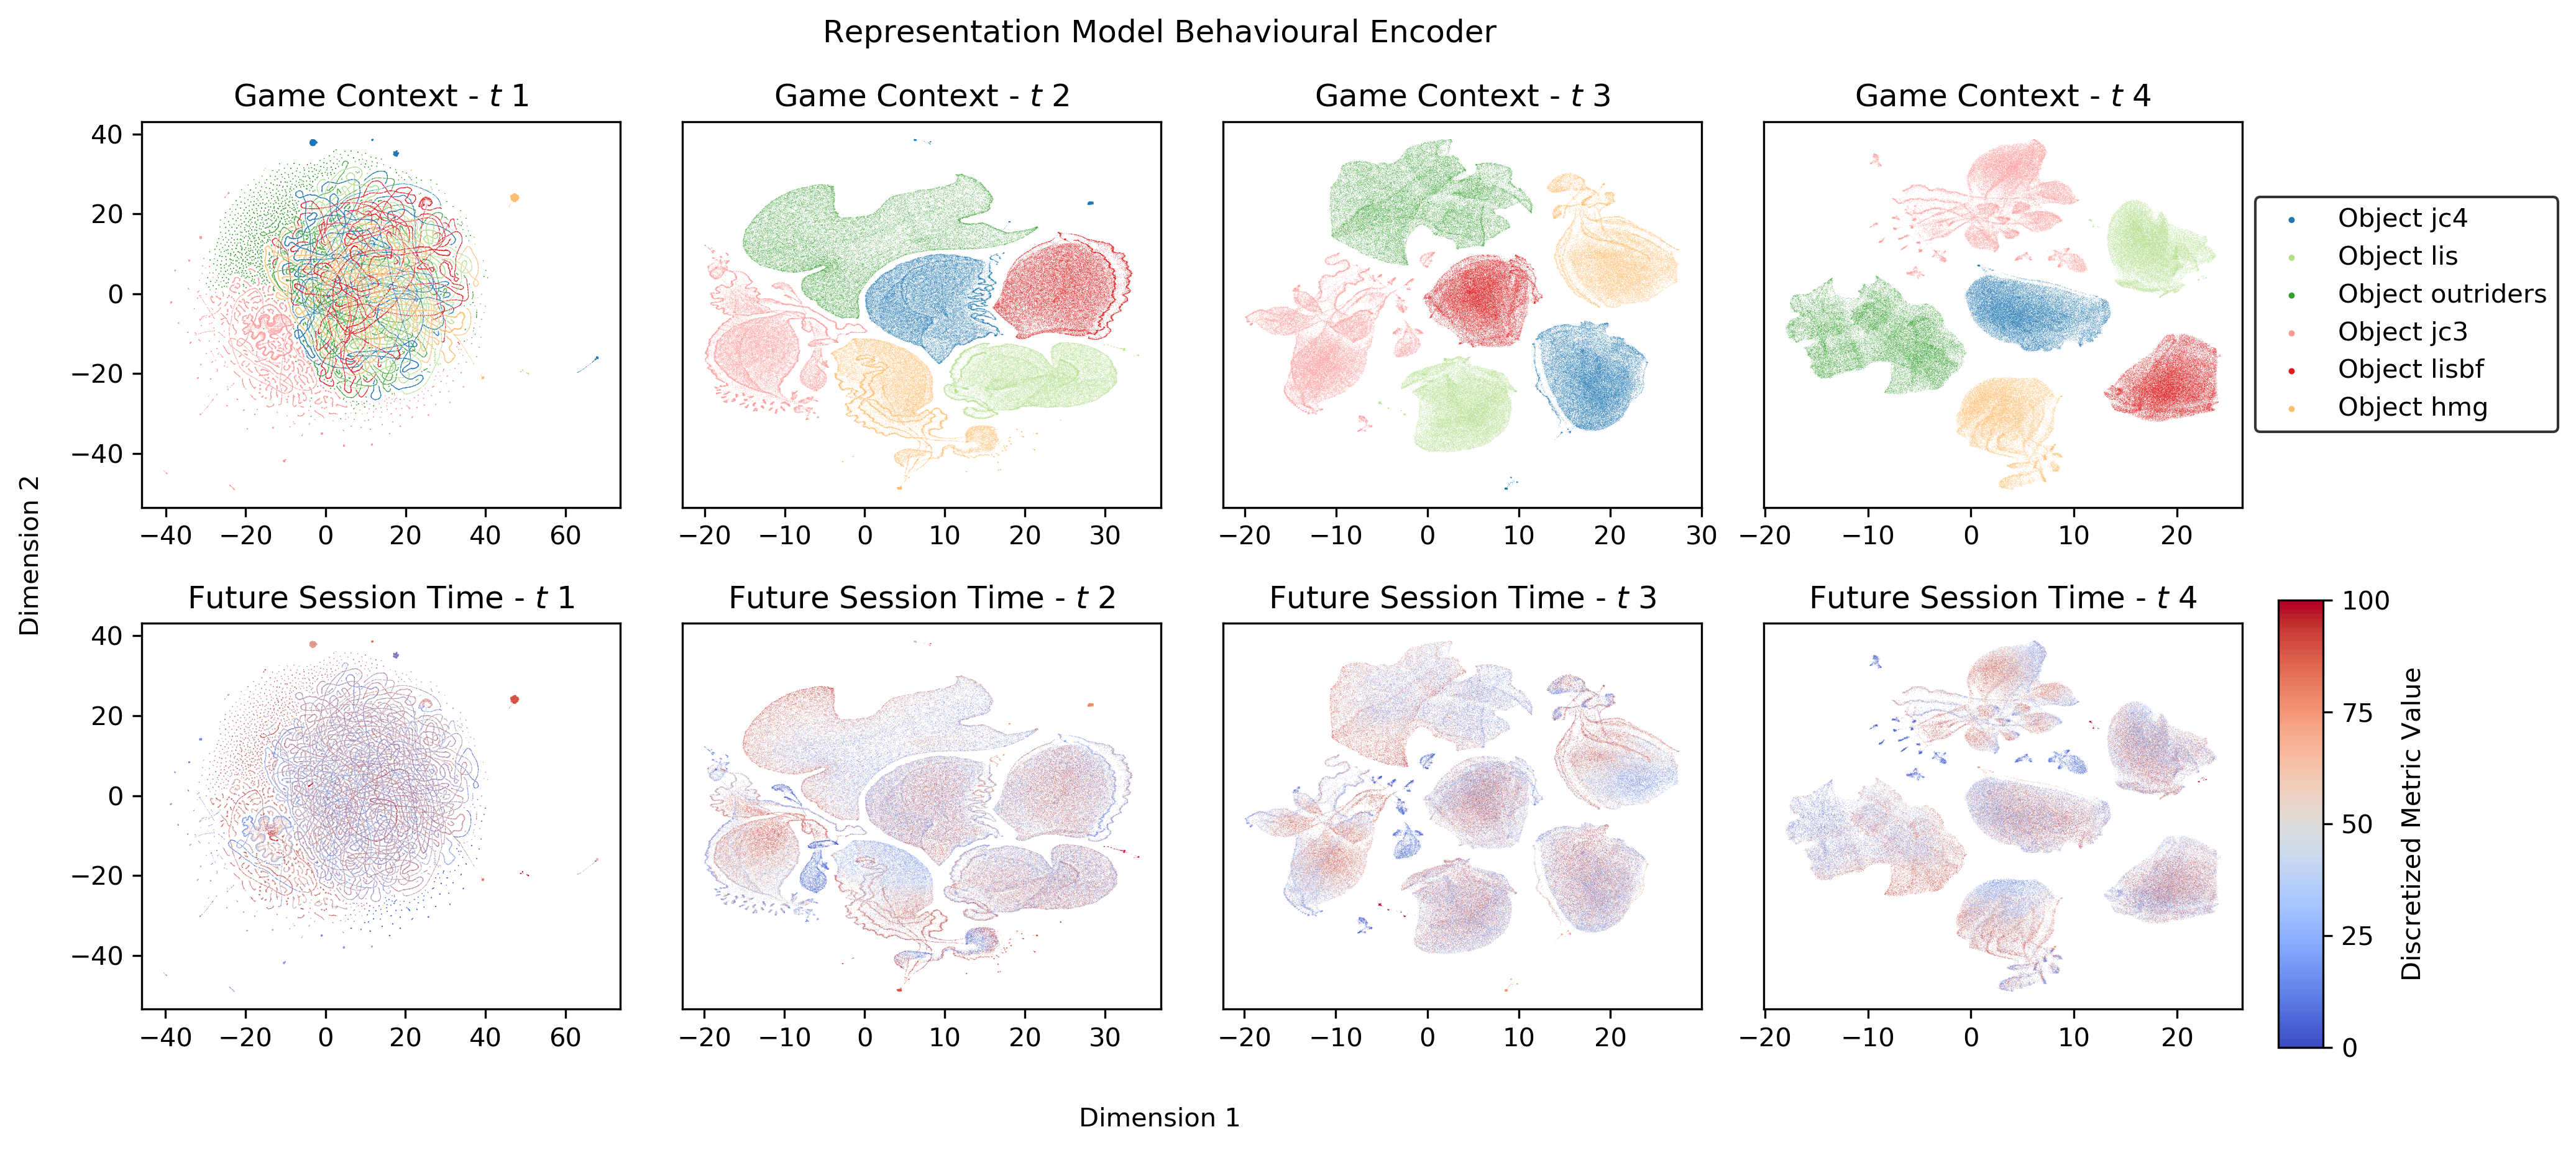
\includegraphics[width=\textwidth]{images/chapter_4/RNN_env_even_0_lstm_layer_features_Future Session Time.png}
\caption[\textbf{Lower dimensional representation of the latent representations generated by the improved version of the RNN architecture from the behavioural metrics}]{Each panel shows a two-dimensional projection of the multi-dimensional representation inferred by the improved RNN architecture at $t1$, $t2$, $t3$ and $t4$. The representations presented in this figure have been generated by the portion of the architecture receiving the behavioural metrics as input. As in Figure \ref{full_panel_temporal}, x and y axes are dimensions individuated by the UMAP algorithm and can be interpreted as a coordinate system where proximity represents similarity between points. Colours in the first row indicate which game object the representation is coming from while those in the second row indicate the discounted sum of future predictions for a single target (i.e. "Future Session Time").}
\label{rnn_env_even_full_beha}
\end{figure}

we can see how the representation generated from the behavioural metrics changes considerably from the simple RNN architecture. Despite the ability to differentiate between game objects is, up to a certain degree, preserved, the quality of the gradient organization is markedly diminished. This is doesn't come as a surprising result: similarly to what happens when covariates are added in a linear model, the behavioural metrics are now only one of the components making up the final representation in charge of producing the model's predictions. It is however worth noticing that the ability to differentiate between individuals with respect to the intensity of their future interactions is not completely removed suggesting the intensity of past interactions still plays a role in determining the intensity of future ones. 

The same cannot be said for the representation generated by the environmental metrics. If we look at Figure \ref{rnn_env_even_full_env} we can see that not just the ability to differentiate between game objects is almost completely disrupted, but also the capacity to distinguish between individuals with high and low expected intensity of future interactions. 

\begin{figure}[!htb]
\centering
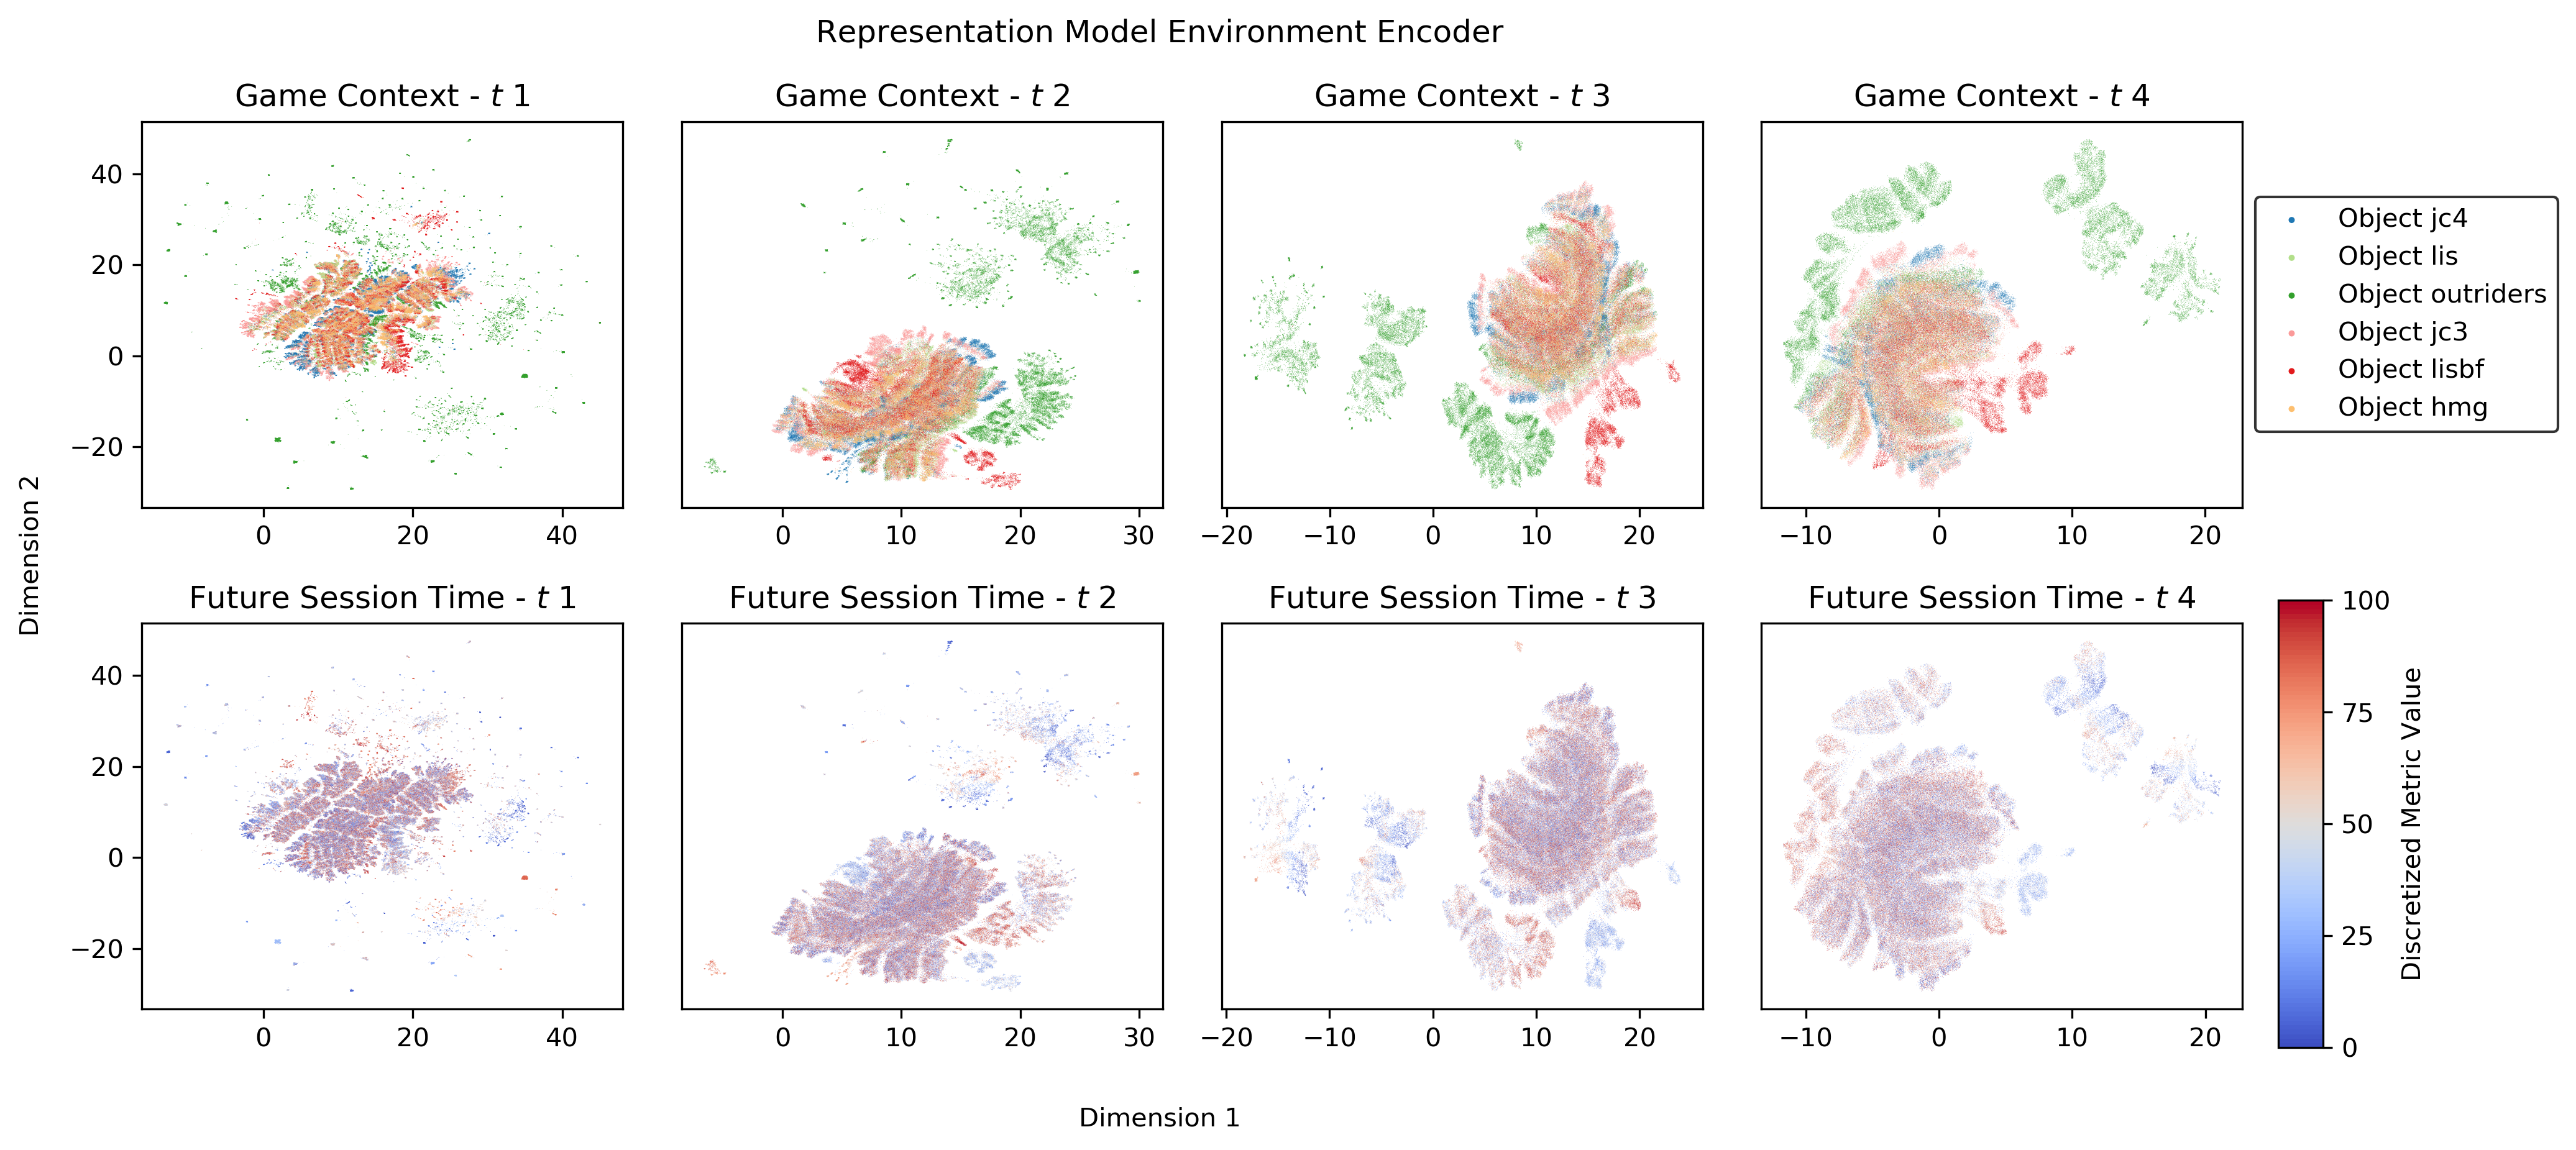
\includegraphics[width=\textwidth]{images/chapter_4/RNN_env_even_0_lstm_layer_env_Future Session Time.png}
\caption[\textbf{Lower dimensional representation of the latent representations generated by the improved version of the RNN architecture from the environmental metrics}]{Each panel show a two-dimensional projection of the multi-dimensional representation inferred by the improved RNN architecture at $t1$, $t2$, $t3$ and $t4$. The representation presented in this figure has been generated by the portion of the architecture receiving the environmental metrics as input. As in Figure \ref{full_panel_temporal}, x and y axes are dimensions individuated by the UMAP algorithm and can be interpreted as a coordinate system where proximity represents similarity between points. Colours in the first row indicate which game object the representation is coming from while those in the second row indicate the discounted sum of future predictions for a single target (i.e. "Future Session Time").}
\label{rnn_env_even_full_env}
\end{figure}

As we anticipated in sections \ref{model_architecture_3} and \ref{modelling_env_and_game_elements}, we did not expect the environmental variables to have strong predictive power on future ammount of gaming behaviour, but rather to act as an absorbing factor for possible noise observed in the behavioural metrics. Or better, we argued that environmental factors might affect the behavioural manifestations of a certain latent state (i.e. attributed incentive salience) both in the past and in the future, but do not play a central role in the shaping of the state itself (i.e. the level of attributed incentive salience). We will expand more on this section \ref{partition_environment}).

Another possibility is that the environmental information do not play a relevant role in generating a latent representation with good predictive power and are just treated as noise by the model. However, by looking at the occasional improvements in predictive performance that they provided in section \ref{results_3}, it seems more plausible that they are to be considered as nuisance metrics supporting the role of the other model inputs. 

The representation generated from the game events information sits in stark contrast to the previous two. Looking at Figure \ref{rnn_env_even_full_events} we can see how different it is from what we observed in Figure \ref{rnn_env_even_full_beha}. The representation appears highly fragmented but with each fragment consistently belonging to distinct game contexts. This suggests the representation attempted to encode the heterogeneity in sequences of game events while maintaining them within the same context.

\begin{figure}[!htb]
\centering
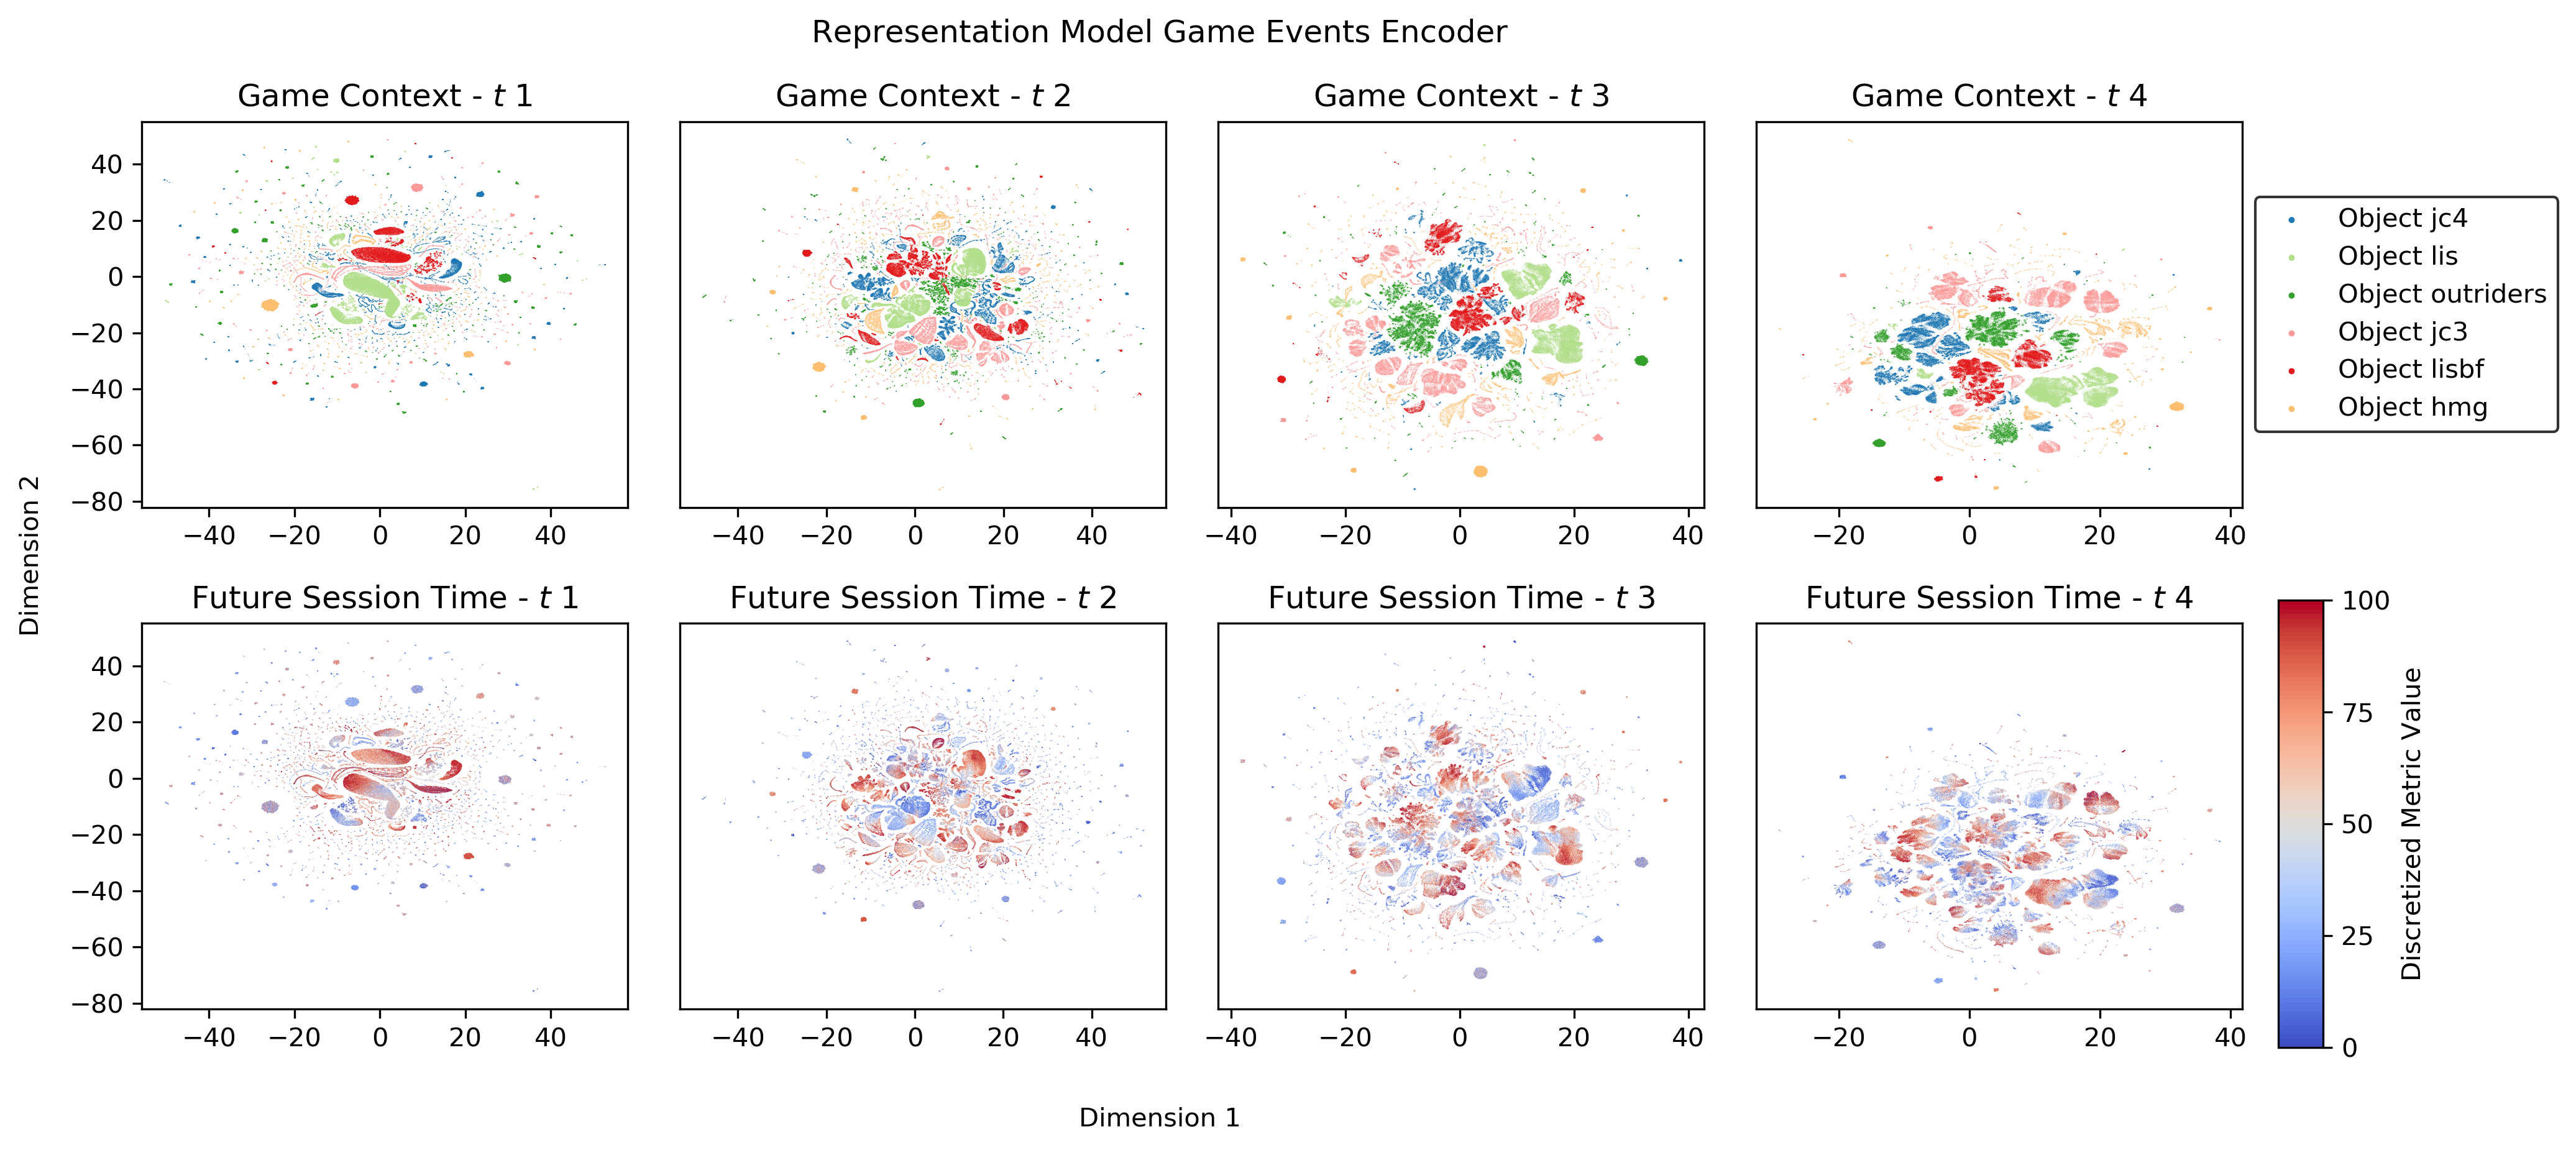
\includegraphics[width=\textwidth]{images/chapter_4/RNN_env_even_0_lstm_layer_events_Future Session Time.png}
\caption[\textbf{Lower dimensional representation of the latent representations generated by the improved version of the RNN architecture from the game events metrics}]{Each panel show a two-dimensional projection of the multi-dimensional representation inferred by the improved RNN architecture at $t1$, $t2$, $t3$ and $t4$. The representation in this figure has been generated by the portion of the architecture receiving the game events metrics as input. As in Figure \ref{full_panel_temporal}, x and y axes are dimensions individuated by the UMAP algorithm and can be interpreted as a coordinate system where proximity represents similarity between points. Colours in the first row indicate which game object the representation is coming from while those in the second row indicate the discounted sum of future predictions for a single target (i.e. "Future Session Time").}
\label{rnn_env_even_full_events}
\end{figure}

The observed level of fragmentation is in line with all the possible sets arising by the combination of the considered game events and their relative frequency of interactions. For example considering the tuple $\{event, frequency\}$ we could have:

\begin{gather}
\label{seq_differences}
    \{\{combat, 10\}, \{explore, 3\}, \{achievement, 2\}\} \\ \nonumber
    \neq \\ \nonumber
    \{\{combat, 2\}, \{explore, 10\}, \{achievement, 5\}\} \\ \nonumber
    \neq \\ \nonumber
    \{\{dialogue, 2\}, \{puzzle, 10\}, \{achievement, 5\}\} \\ \nonumber 
    \neq \\ \nonumber
    \dots
\end{gather}

This type of behaviour is comparable to what can be observed when analyzing the word embeddings of different text corpora (e.g. see the Open Syllabus project \cite{opensyllabus}) and suggest that the architecture was able to discern differences in the sequential choices made by the individuals when interacting with different in-game elements.

What is most interesting however is that among the representations inspected so far, the one generated from the game events metric is the one that best preserves the gradient organization observed for the simple RNN architecture. This suggests that the sequences of observed interactions with specific in-game mechanics plays a role in differentiating between individuals with respect to the expected intensity of their future interactions with a specific game object. This, in turn, is something that we anticipated in sections \ref{factors_engagement} and \ref{modelling_env_and_game_elements} and that is in line with previous findings in the videogame literature \cite{makarovych2018like}.

Finally, when looking at the shared representation in Figure \ref{rnn_env_even_full_shared}, we can see how it resembles the one generated by the simplified version of the RNN architecture with the only difference being a more clearly defined gradient organization. This representation is functionally equivalent to the one extracted by the simplified RNN architecture (i.e. it is used for performing multi-task learning) and is hypothesized to approximate the manifold structure of attributed incentive salience.

\begin{figure}[!htb]
\centering
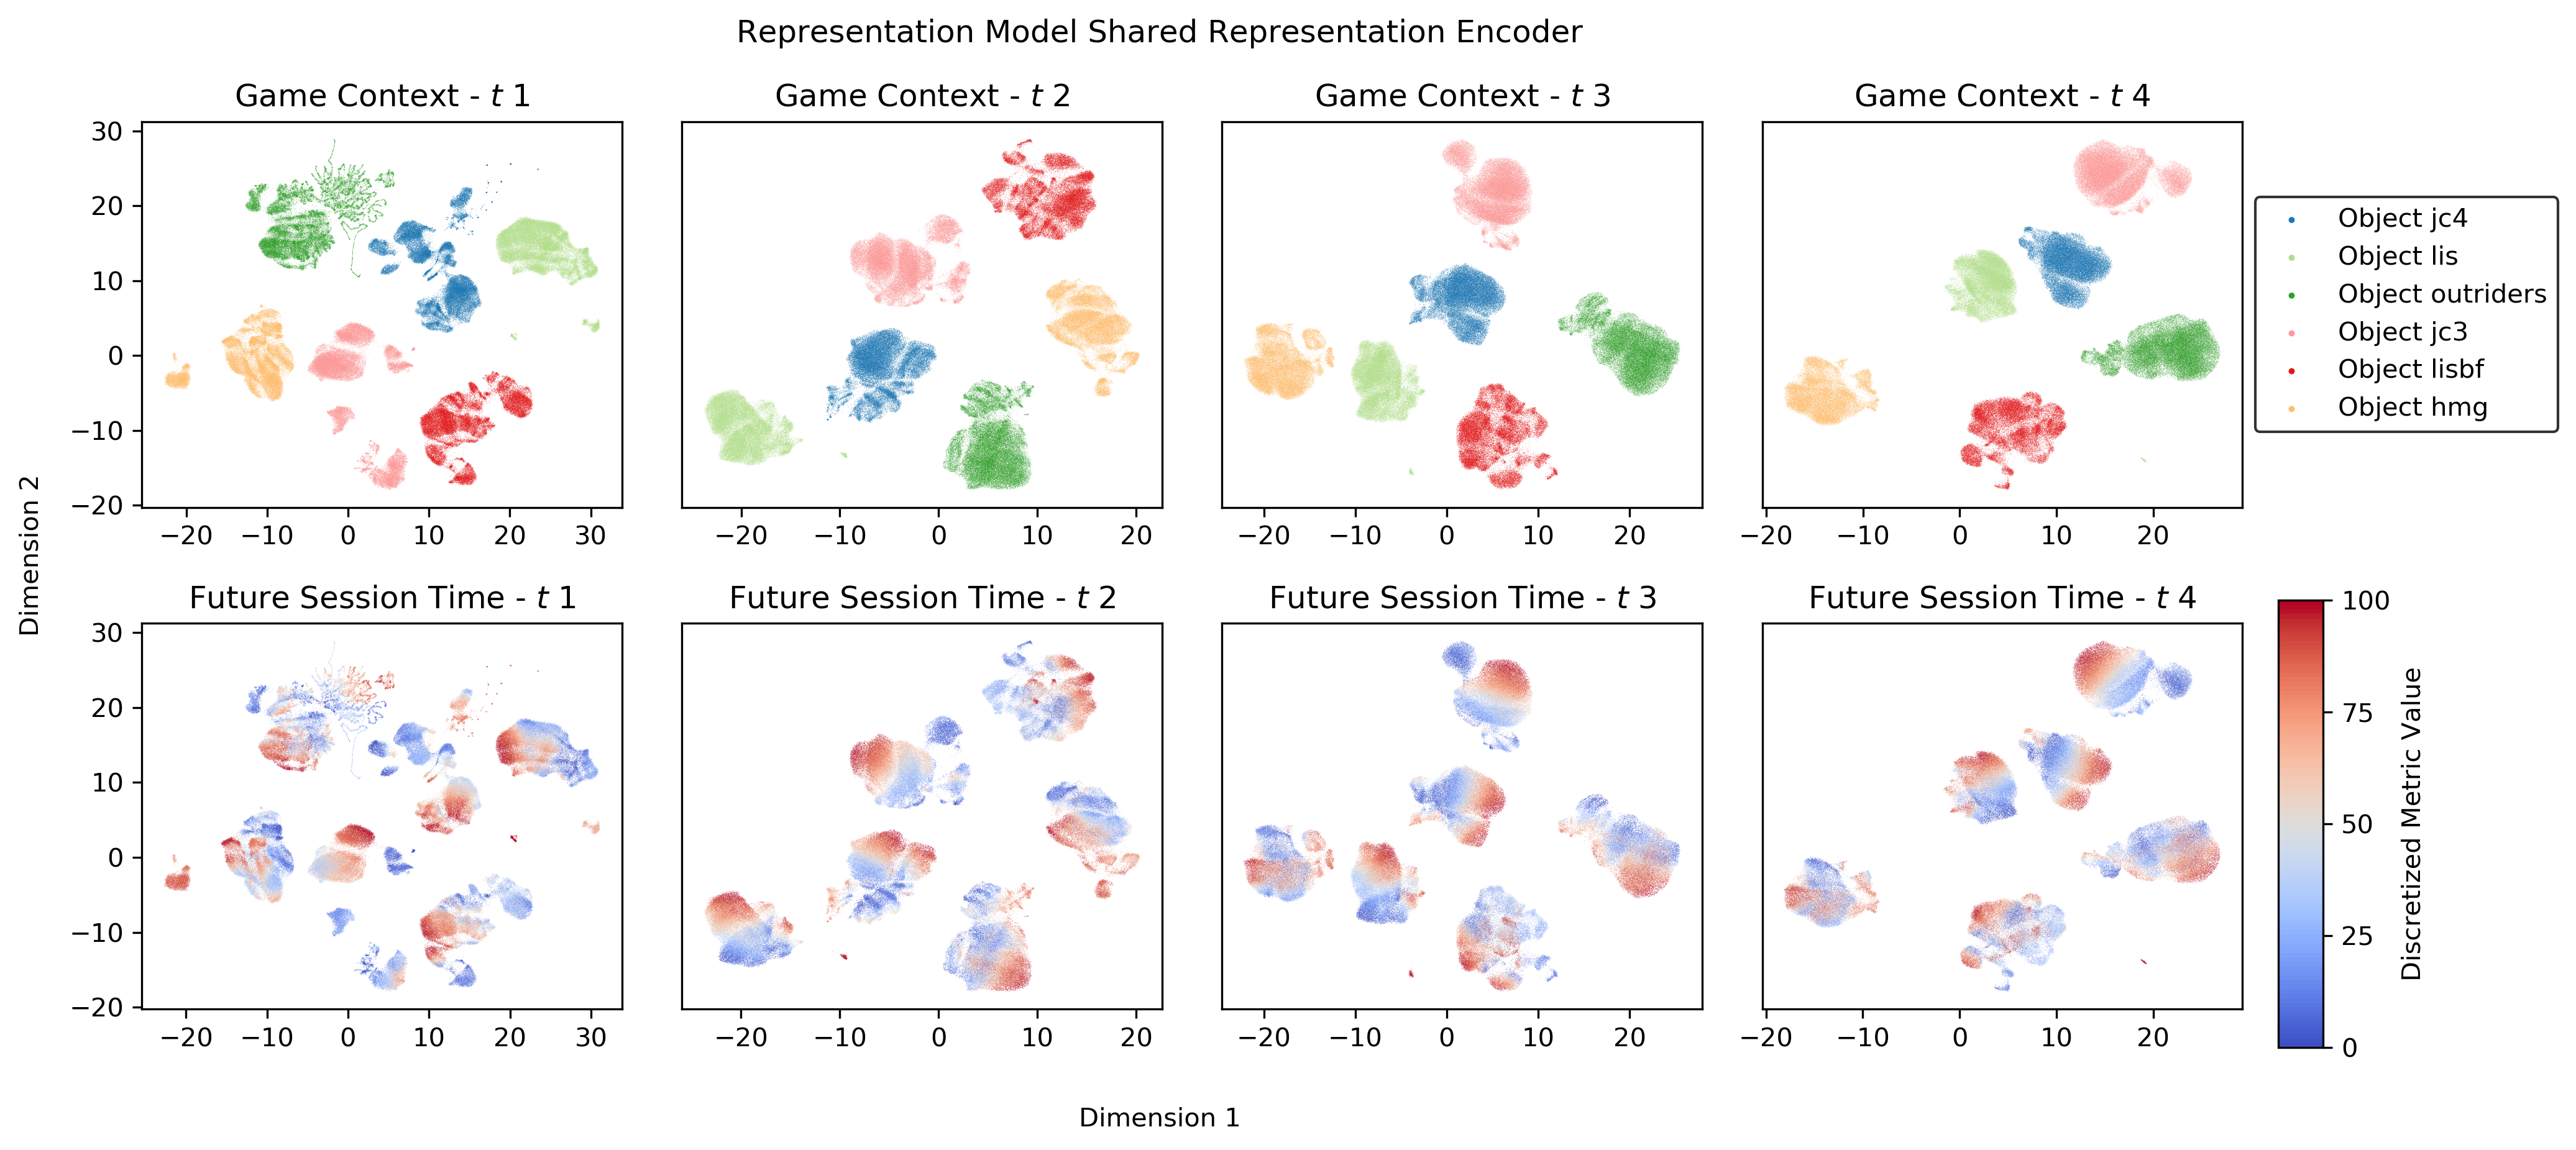
\includegraphics[width=\textwidth]{images/chapter_4/RNN_env_even_0_lstm_layer_shared_Future Session Time.png}
\caption[\textbf{Lower dimensional representation of the shared latent representations generated by the improved version of the RNN architecture}]{Each panel show a two-dimensional projection of the multi-dimensional representation inferred by the improved RNN architecture at $t1$, $t2$, $t3$ and $t4$. The representation presented in this figure has been generated by the portion of the architecture receiving as inputs the representations associated with the behavioural, environmental and game events input and is the one hypothesized to approximate the manifold structure of attributed incentive salience. As in Figure \ref{full_panel_temporal}, x and y axes are dimensions individuated by the UMAP algorithm and can be interpreted as a coordinate system where proximity represents similarity between points. Colours in the first row indicate which game object the representation is coming from while those in the second row indicate the discounted sum of future predictions for a single target (i.e. "Future Session Time").}
\label{rnn_env_even_full_shared}
\end{figure}

This qualitative improvement can be better appreciated when comparing the representation generated by the two version of the RNN architecture, color coded using the ground truth values rather than the predictions provided by the models. Looking at Figure \ref{rnn_predictive_comparison}

\begin{figure}[ht]
\centering
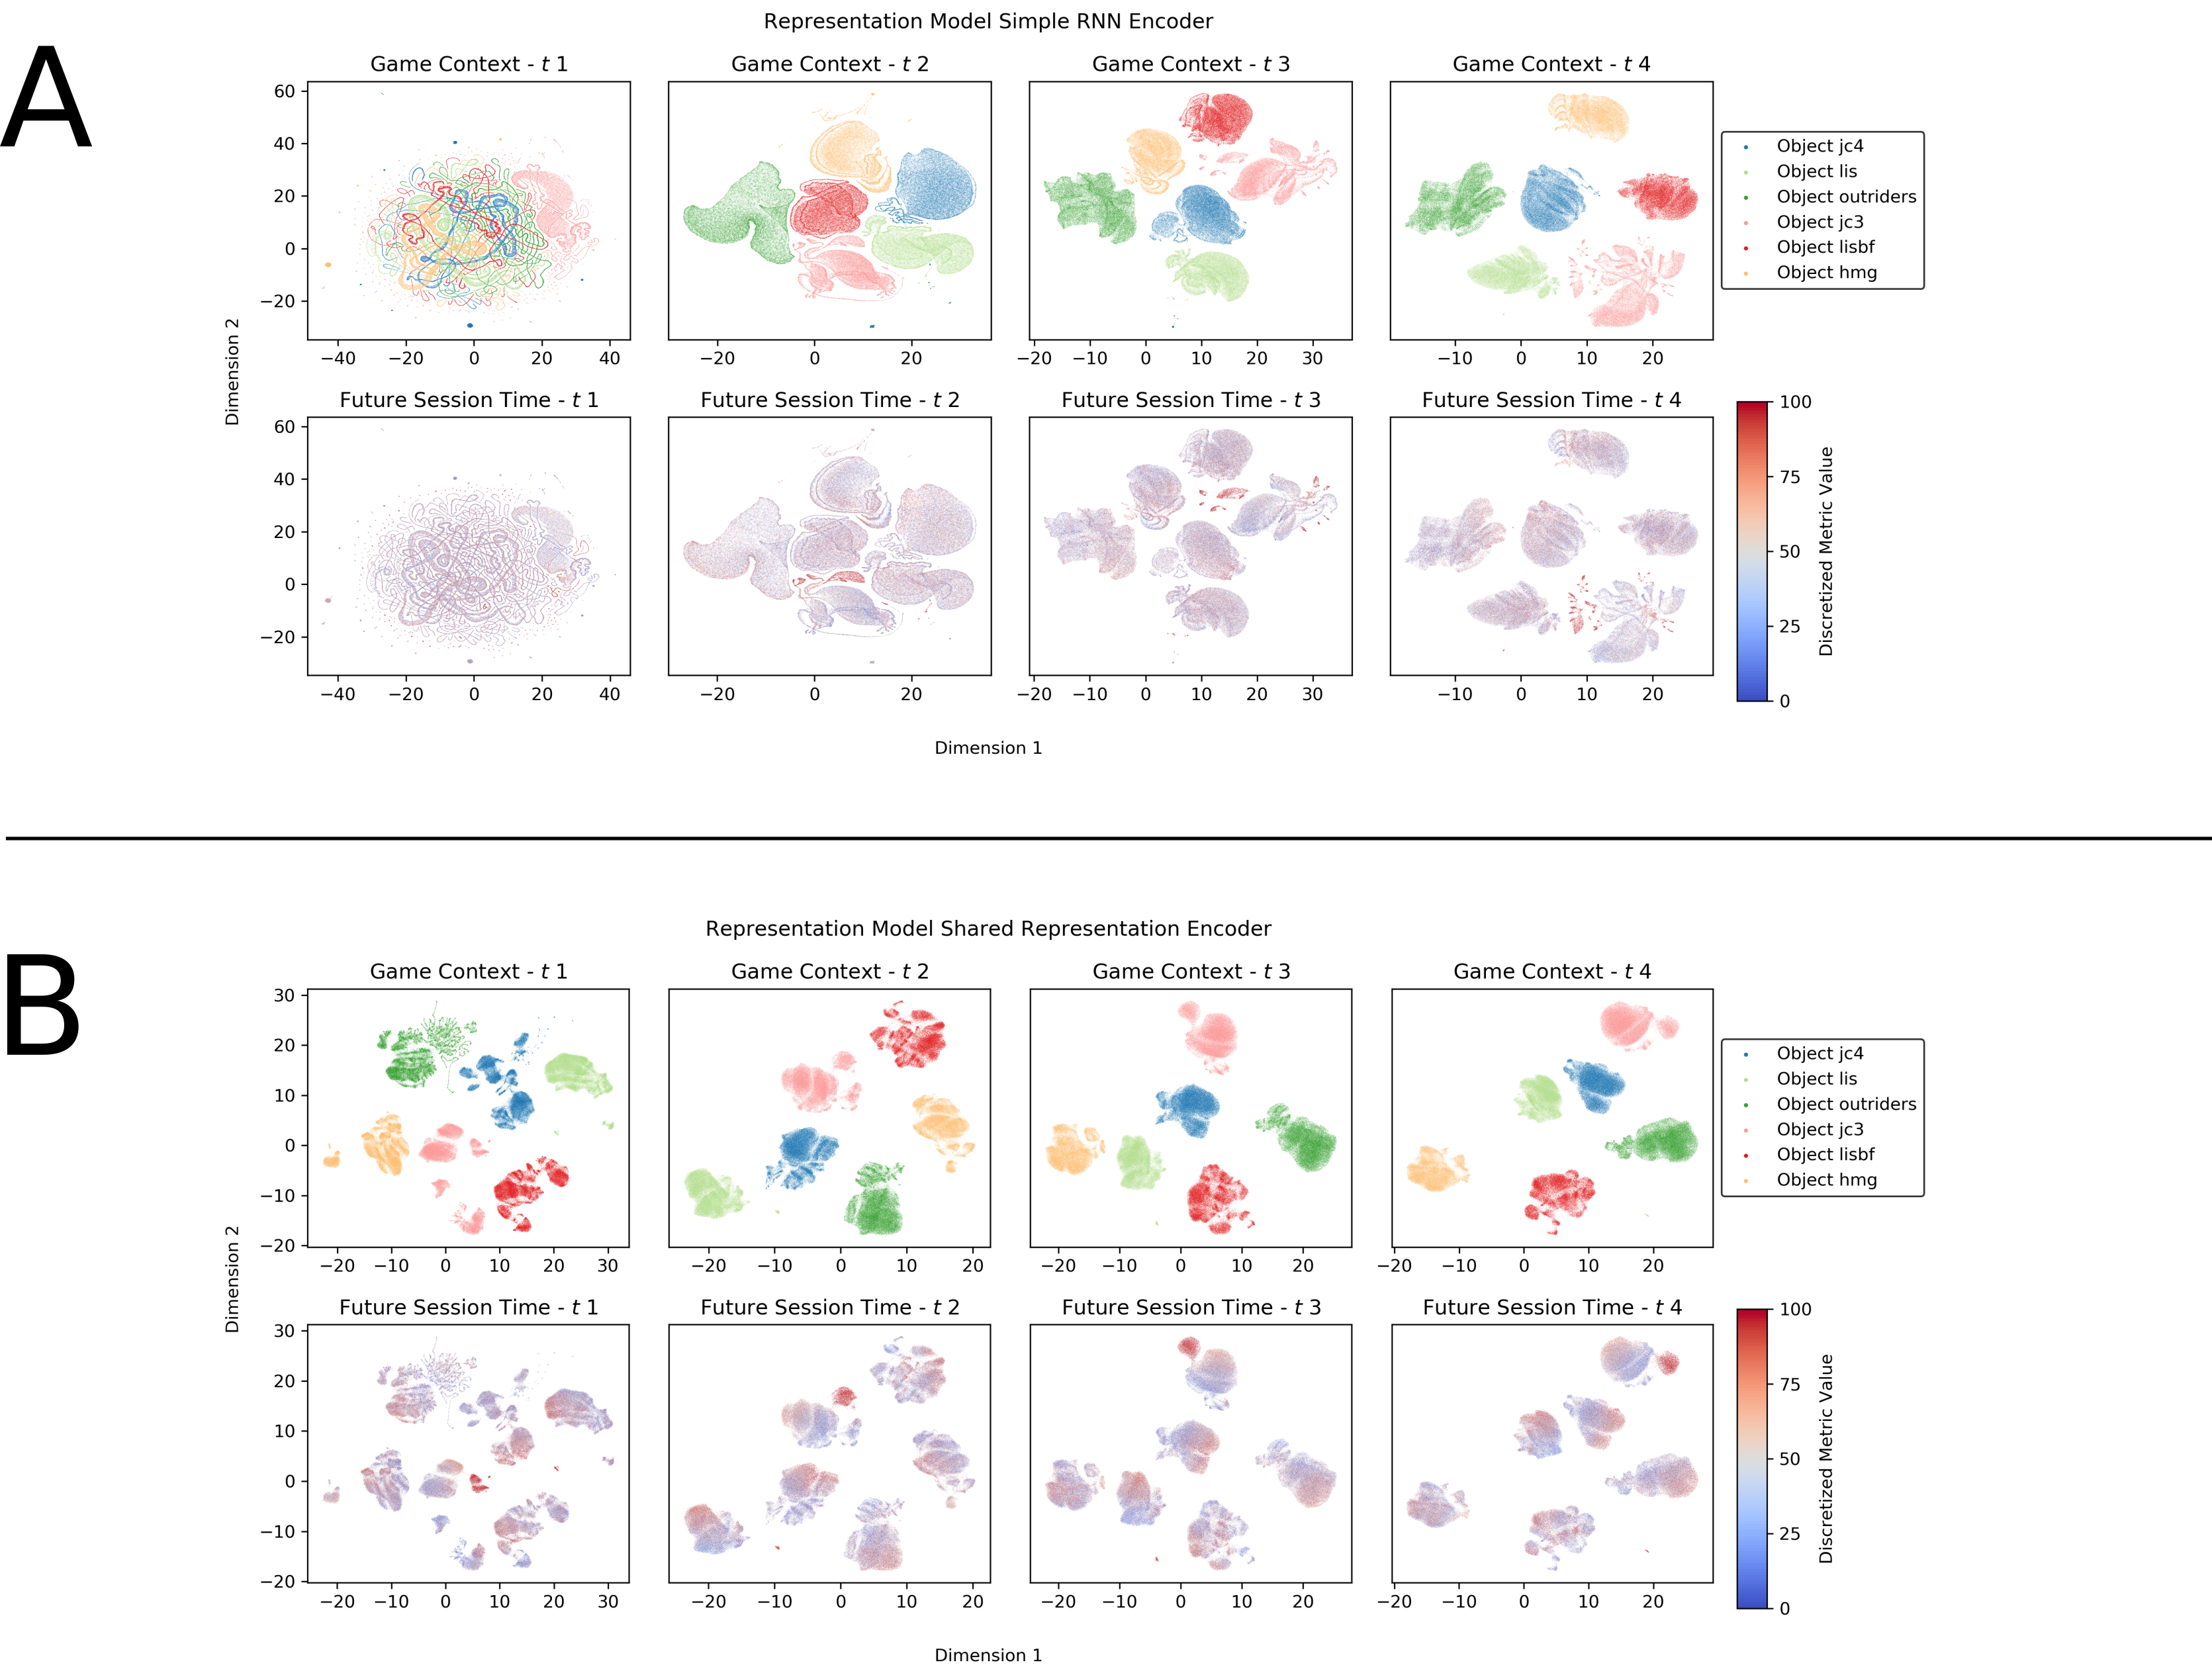
\includegraphics[width=\textwidth]{images/chapter_4/rnn_predictive.png}
\caption[\textbf{Differences in predictive power between the representations generated by the RNN architecture and its improved version}]{The figure show the two-dimensional projection, produced by UMAP, of the multi-dimensional representation generated by the RNN architecture and its improved version at $t1$, $t2$, $t3$ and $t4$. Both representations have been extracted by the portion of the architecture hypothesized to approximate the manifold structure of attributed incentive salience. Panel A refers to the RNN architecture while panel B to its improved version (including environmental and game event covariates). As in Figure \ref{full_panel_temporal}, x and y axes are dimensions identified by the UMAP algorithm and can be interpreted as a coordinate system where proximity represents similarity between points. Colours in the first row indicate which game object the representation is coming from while those in the second row indicate the discounted sum of future ground truth values for a single target (i.e. "Future Session Time").}
\label{rnn_predictive_comparison}
\end{figure}

we can see how the simplified RNN architecture shows a greater level of disruption in the gradient like organization than its improved version, suggesting that this last one is likely to be a better approximation of the functional properties of the latent state (i.e. the level of attributed incentive salience) that generated the observed behaviour. By looking at figure \ref{rnn_env_even_full_shared}, we can notice how the topological characteristics of the previous three representations are replaced by the global-local organization that we described in \ref{functional_properties}. This consistency corroborates the idea that this type of organization is the most suitable one for the type of predictive task that the two architectures are aiming to solve.

\section{Partition Analysis}
\label{partition_analysese}
In order to gather additional insights on the functional properties of the representations generated by our architectures, we attempted to map what inferred by the models back to the observable behavioural space. As specified in section \ref{manifold_learning} these representations are derived from the input metrics and can be interpreted as coordinates on the manifold structure inferred by the architectures. In this view, partitioning them allows identify areas of the manifold holding information about the history of interactions between an individual and a given video game object. Moreover, since the manifold is constructed to be informative of the intensity of future interactions, different partitions might represent not just variations in the input metrics (e.g. differences in the sequences of events triggered in the game) but also in the level of attributed incentive salience. By individuating the set of metrics that contributed to defining the topology of different regions of the inferred manifold we may hope to gather insights on their role in determining the intensity of future behaviour. 

To perform the mapping, we opted for an unsupervised approach and conducted a partition analysis on the representations extracted by the different encoders. 
To partition the data, we decided to apply Mini-Batch K-Means \cite{sculley2010web}, a variation of K-Means, to the representation extracted by the three encoders mentioned in section \ref{representation_analysis}. Given a dataset, the algorithm attempts to divide it by iteratively moving $k$ centroids so as to reduce variance within each partition. The choice of Mini-Batch K-Means was dictated by the fact that it is one of the few distance-based algorithms that scales to very large datasets. The reason for choosing a distance-based algorithm can be found in paragraph \ref{manifold_learning}, there we specified how distance in the manifold structure inferred by an ANN can be interpreted as a measure of similarity between its input with respect to the objective function that the model is trying to minimize. 

To select the optimal $k$ value, we first fitted the algorithm with a varying number of centroids (i.e. 2 to 10) and computed the associated inertia, a measure of within cluster variance (see \ref{inertia}. Since inertia tends to zero as $k$ approaches the number of points in the dataset, we defined the optimal number of partitions as the value of $k$ at which the inertia reached its "elbow" or maximum curvature \cite{satopaa2011finding}. This allows us to identify the point at which increasing the number of partitions provides diminishing returns in terms of within cluster variance reduction. Despite the fact that this procedure might be prone to errors or imprecision (e.g. the elbow might be non-unique or change depending on the maximum number of considered centroids) we thought it would be preferable to an arbitrary choice. 

Every instance of Mini-Batch K-Means was initialized 3000 times at random and ran for a maximum of 3000 epochs. The input data were re-scaled to have zero mean and unit-variance and passed to the algorithm in random batches of size $(512 \times h)$. The associated behavioural profiles were found by applying this methodology separately to each game object and retrieving, for each partition, the expected deviation of all the behavioural metrics from their relative mean (computed along the temporal dimension) in each game context. In order to have an indication of the quality of the individuated partitions, we decided to computecomputed the average silhouette score (see appendix \ref{silhouette}). The silhouette score can be interpreted as an index of cluster cohesion. It is bounded between -1 and 1 and a high value indicates that, on average, all the considered points are well matched to their own partition and poorly matched to neighboring partitions, while the reverse is true for low or negative values. 

We will first focus on inspecting the partitions derived from the representations generated by encoding the behavioural metrics using the RNN architecture and its improved version. We will subsequently move onto the partitions associated with those representation related to environmental and game events covariates. When analysing the obtained partitions we will focus only on those related to the game object $outriders$, results related to other game objects will be reported in appendices \ref{partitions_behavioural}, \ref{partitions_environmental} and \ref{partitions_game_events} and mostly used for drawing general remarks. 

The Mini-Batch K-Means implementation used for this analysis was provided by the python library scikit-learn \cite{scikit-learn}. All the analyses were conducted using Python programming language version 3.6.2 \cite{10.5555/1593511}.

\subsection{Partitioning the representation associated to the behavioural inputs}
\label{partition_behaviour}
As we can see from Figure \ref{partition_rnn_behaviour}, following the methodology outlined in section \ref{partition_analysese}, among all the Mini-Batch K-Means runs, the one with $k=4$ was identified as the optimal one for both representations. All the partitions were associated with a distinct behavioural profile, each one with its own offset and temporal evolution. It is relevant to note that the profiles identified for the two representations are virtually identical (apart from small variations in some of the metrics). However the representation extracted by the improved version of the RNN architecture appears to allow for qualitatively superior (i.e. more compact) partitions as highlighted by the higher average silhouette score.

\begin{figure}[!htb]
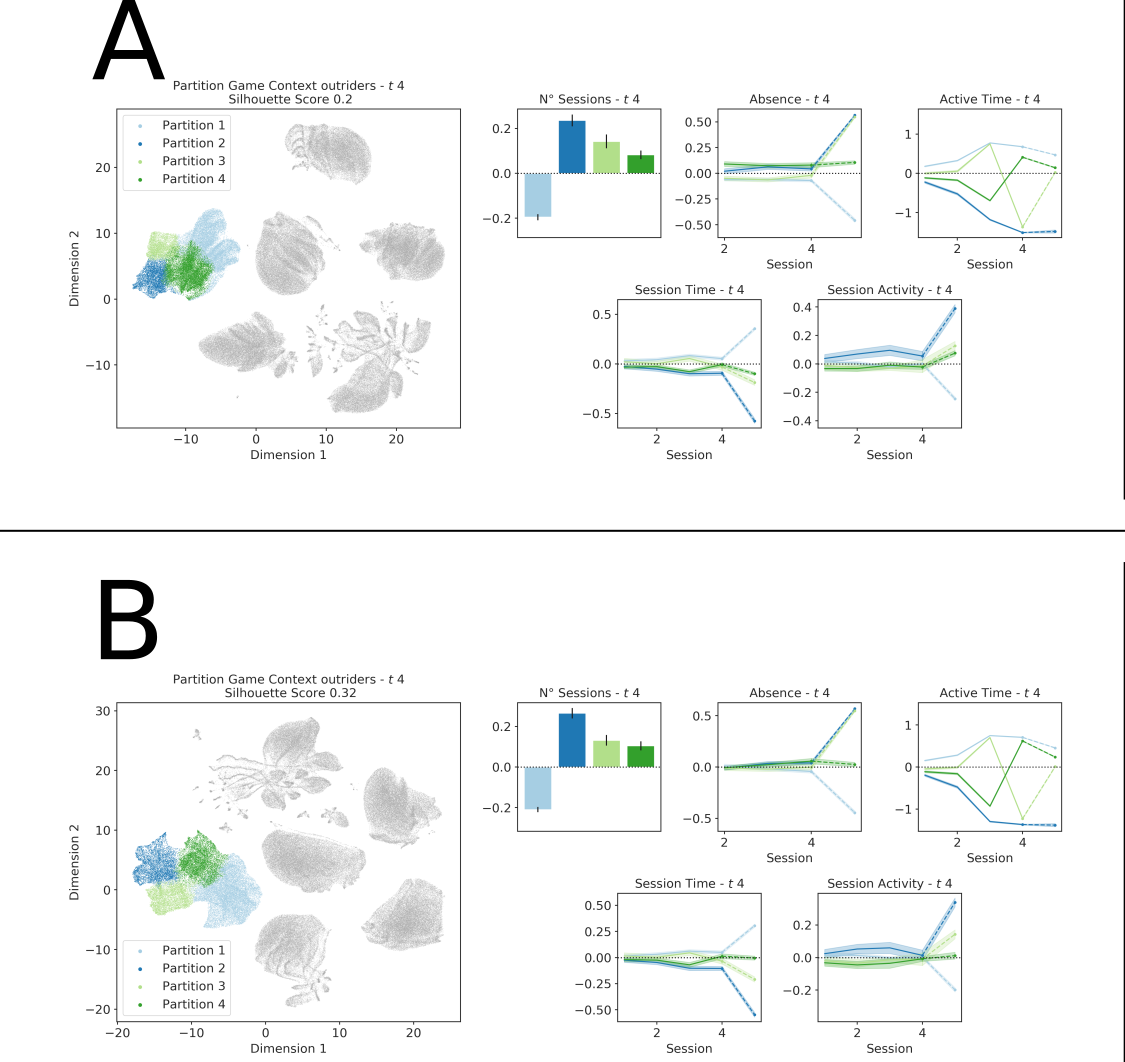
\includegraphics[width=0.7\textwidth]{images/chapter_4/clust_beha.png}
\centering
\caption[\textbf{Partitions of the representations generated by the RNN architectures from the behavioural metrics}]{The two panels shows the individuated partitions and associated behavioural profiles at $t4$. The big panels report the same UMAP reduction presented in the last column of Figure \ref{full_panel_temporal}. Each dot is the representation associated with a particular individual and is colour coded based on the partition to which it belongs. Small panels represent the temporal evolution of the considered behavioural metrics for each individuated partition. The panel showing  N°Sessions only reports the prediction produced by the model as the number of preceding session is constant for all the partitions. The x axis reports the game sessions while the y axis the value assumed by the considered metric at a specific point in time. The y axis is expressed in terms of number of standard deviations from the game population mean (i.e. z-scores). Each line indicates the mean z-score while the shaded area around the line its 95\% confidence interval. The solid part of each line indicates the portion of the temporal series observed by the model (i.e. the input) while the dotted part the predictions produced at that point in time. The first columns shows the partitions associated with the representation extracted by the RNN architecture while the second those associated with the representation extracted by the version of the RNN architecture that included environmental and game events covariates. Each row indicates the partitions identified for the six considered game contexts.}
\label{partition_rnn_behaviour} 
\end{figure}

At a global level, the four partitions seem to belong to two general groups: a group with a high propensity to produce future interactions (i.e. partitions 1 and 2) and a group with low propensity (partitions 3 and 4). Noticeably, when looking in detail at each specific partition they appear as variations on the macro group they belong to. Interestingly the percentage of Session Time spent actively interacting with the game object (i.e. Active Time) and the expected N°Sessions seem to be a relevant components in this more granular characterization. 

We will now report examples of the type of behavioural "phenotype" that we were able to derive from the partition analysis. However, Given the unsupervised nature of the adopted methodology and the lack of any strong a-priori expectations on the profiles' outlook, we suggest to interpret them with cautions and consider them as the result of a purely exploratory analysis.

\paragraph*{\textbf{Partition 1}} represents individuals producing high intensity interactions (see Session Time) at a high frequency (see Absence). The high amount of Active Time highlights how the individuals were actively interacting with the game object. The individuals in this partition are projected to produce a number of future interactions that is below average while maintaining a high intensity profile. It can be speculated that the history of high intensity interactions reflected a positive propensity towards the game. This might have prompted individuals in this partition to consume most of the available contents in the game leading to a reduced amount of expected future interactions (i.e. N° Sessions).

\paragraph*{\textbf{Partition 2}} describes individuals that have a history of very infrequent (see Absence) and brief interactions with burst of activities and long idle times (they have the lowest Active time among the individuate partitions). These individuals are expected to maintain this trend in the future although producing a number of interactions that is largely above the average. An hypothetical explanation might see individuals in this partitions constituting a variant of those in Partition 1. The high frequency and intensity of interactions could suggest an eagerness to interact with the game object. This, combined with the low amount of consumed content (see Session Time and Active Time) could explain the projected high amount of future interactions.

\paragraph*{\textbf{Partition 3}} includes individuals whose interactions have been very frequent and average both in terms of length and amount of activity until session 3. From there, a burst in both the length and active time can be observed concomitant with a reduction in latency before the following interaction. This is followed by a re-bounce effect with a marked reduction in the length and intensity of the next interaction. These individuals are predicted to produce a number of future interactions slightly above average while also maintaining a low intensity profile. These individuals might have started with a normal propensity towards the game which suddenly increased around session 3 and had a "physiological" downturn around session 4. 

\paragraph*{\textbf{Partition 4}} contains individuals producing the least intense and frequent interactions. With the only exception of a brief increase in active time around session 4. These individuals are estimated to produce a number of future interactions just above average while maintaining the original low intensity profile. These individuals started and maintained a low intensity profile, suggesting a negative propensity toward the game. 

It is interesting to note that despite the fact that the partitions identified for the various game objects always show the two "macro groups" mentioned above, their finer grain characterizations (i.e. the behavioural profiles extracted from the partitions) vary between game contexts suggesting the presence of a possible interaction (see Appendix \ref{partitions_behavioural}).

Although the individuated profiles can provide valuable information on the behavioural "fingerprint" of group of individuals, the most relevant and reliable information can be found in the relationship between the considered metrics. We observe that Session Time and Session Activity are usually highly correlated. Low Absence seems to be a good indicator of the propensity to produce more interactions in the future. Similarly, high Absence seems to be associated with a general history of low intensity interactions. It is also worth noting that variations in this metric seem to follow and be proportional to increases and decreases in interactions' intensity. 

We can also notice how there is often (but not always) a very high correspondence between the profiles associated with the representations generated by the two versions of the RNN architecture. However, looking at the average silhouette score values, it seems that including environmental and game event covariates helps to generate tighter and more consistent partitions. This might have been driven by mechanism similar to one that we find in conventional linear models: by including appropriate covariates it is possible to obtain more reliable and robust estimates of a specific coefficient of interest \cite{gelman2020regression}.

\subsection{Partitioning the representation associated to the environmental covariates}
\label{partition_environment}
Looking at Figure \ref{partition_rnn_env} we can see the partitions individuated by the Mini-Batch K-Means for the representation generated from the environmental metrics. Given that all the entries included in our dataset were logged using the same time zone (i.e. CEST) we decided to focus in this analysis only on individuals playing from Central European countries. By looking at Figure \ref{partition_rnn_env}A we can observe how individuals tend to distribute their interactions with a game object differently depending on the day of the week or the hour of the day. This finding is not surprising but is in line with the idea mentioned in sections \ref{estpred_motivation_engagement} and \ref{modelling_env_and_game_elements}: the environment in which an interaction (here, between an individual and a game object) occurs help to determine its observed behavioural intensity. 
\begin{figure}[!htb]
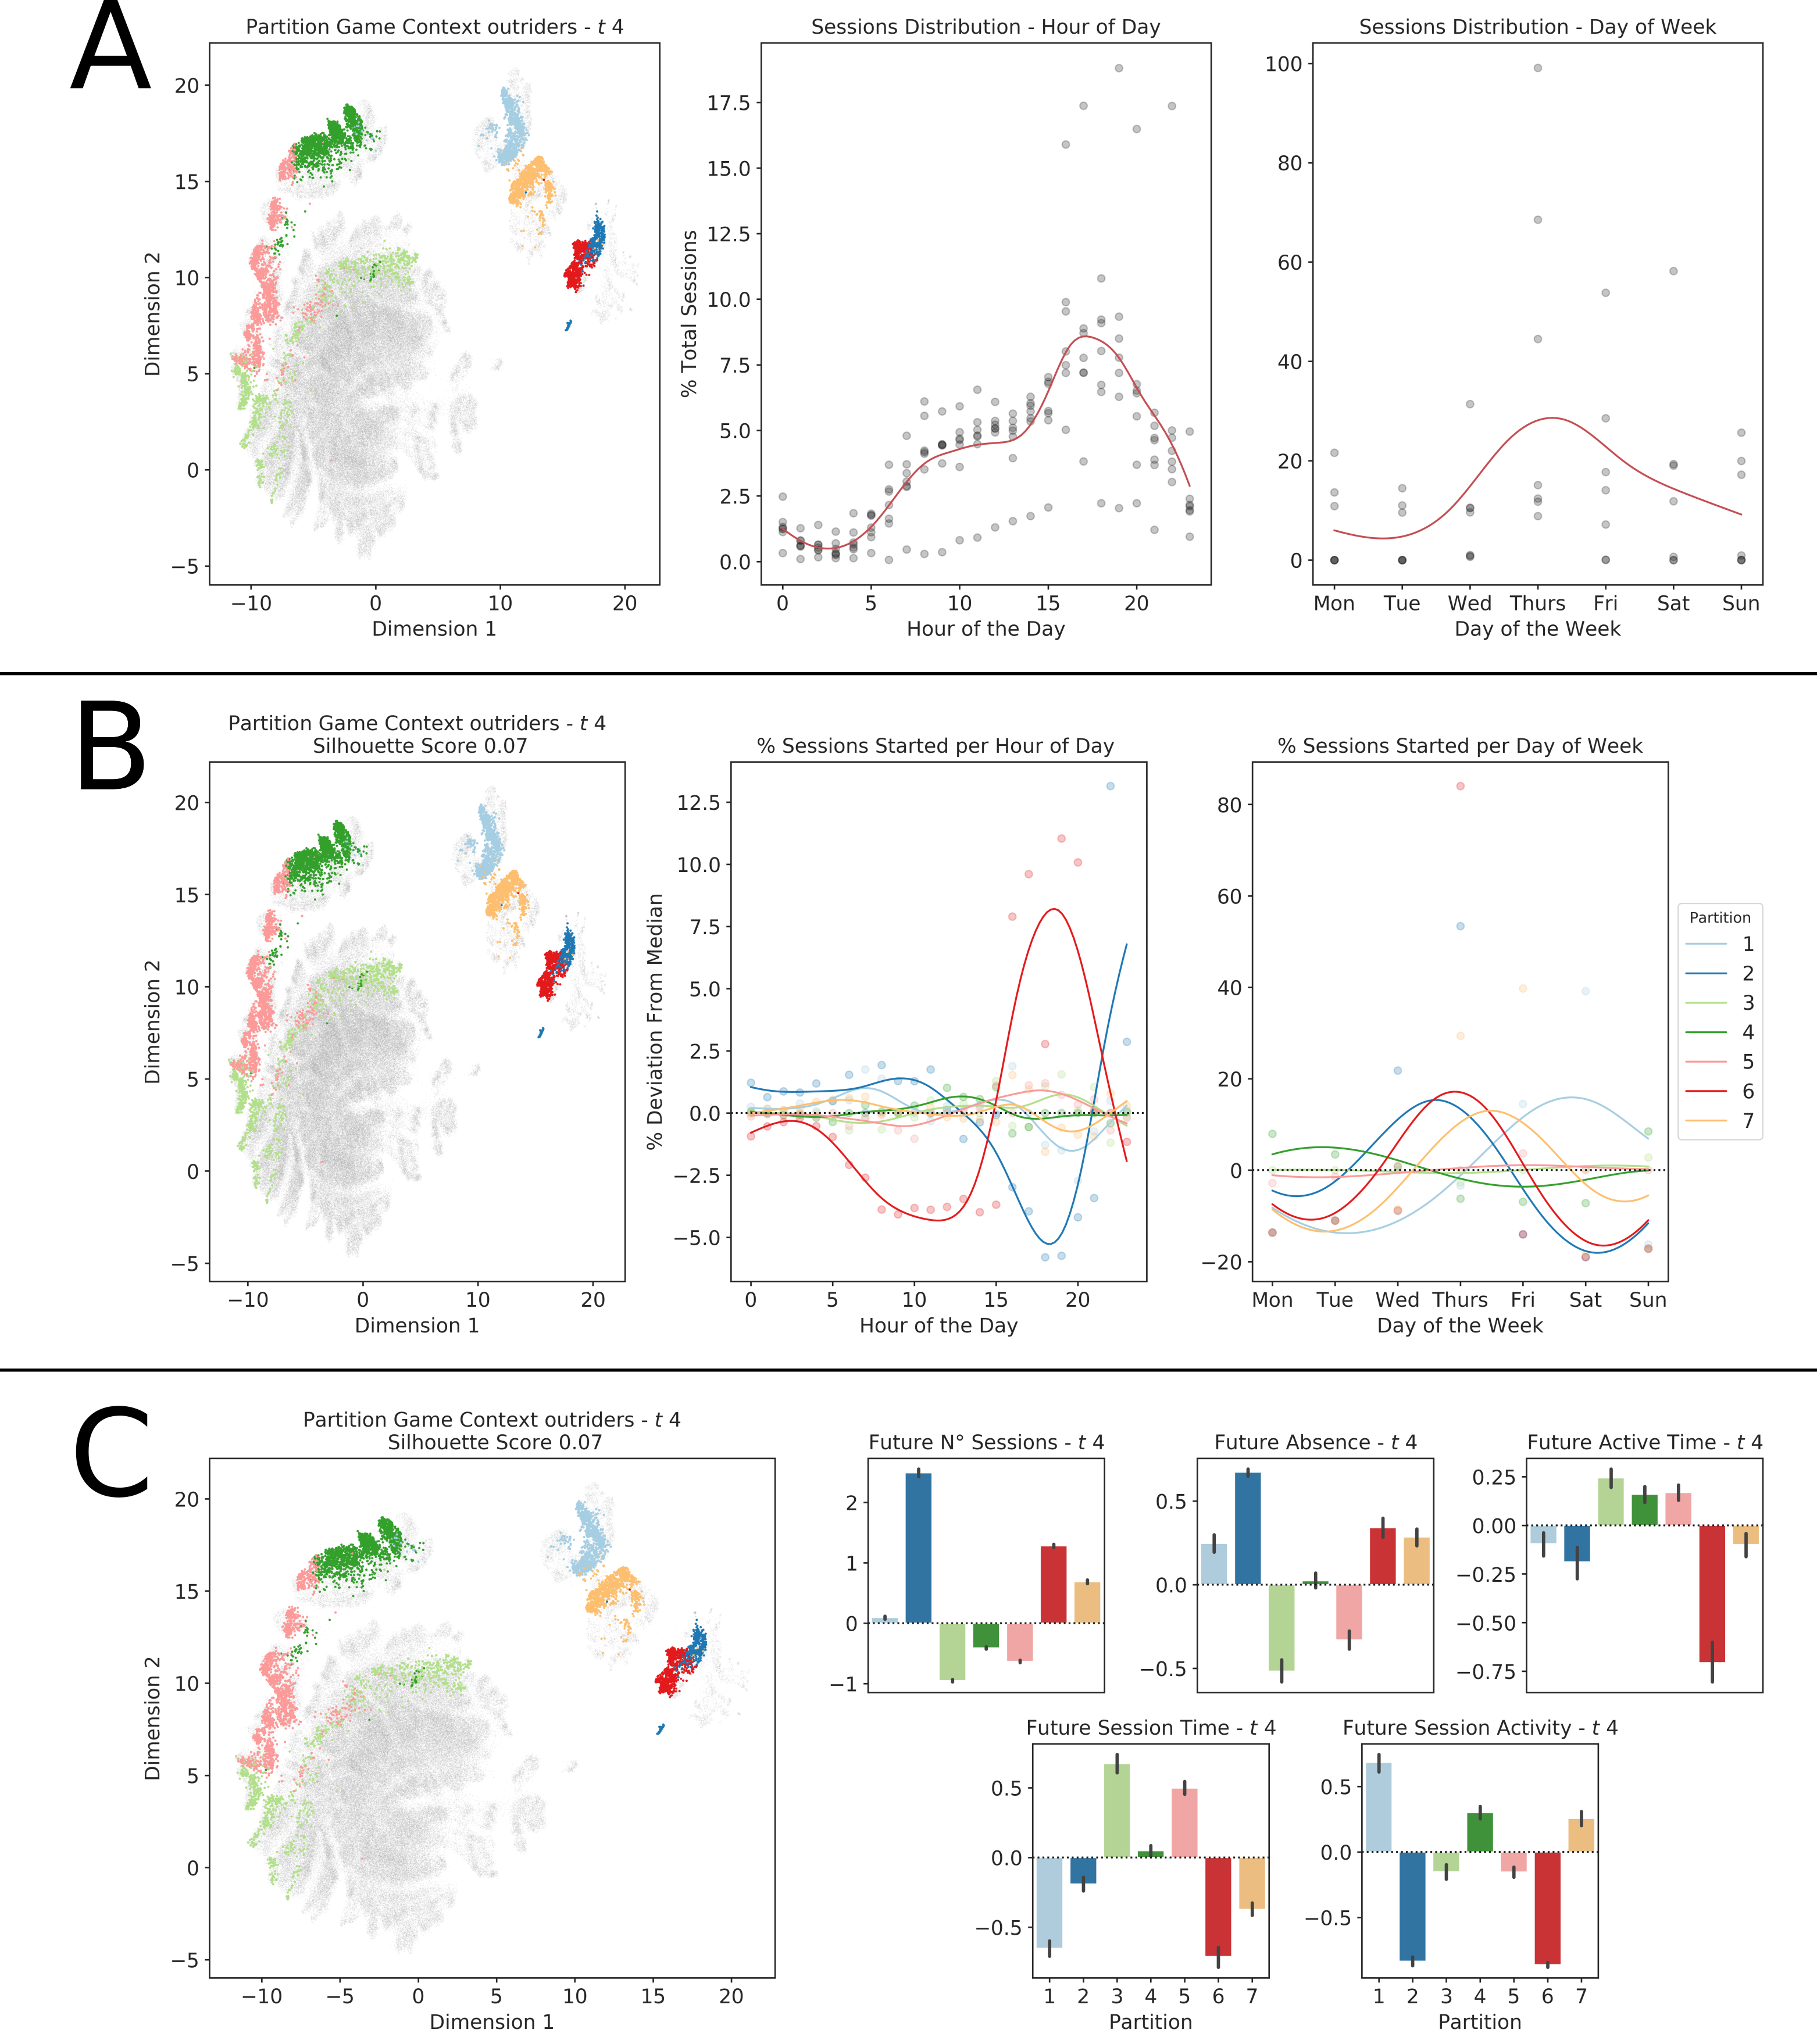
\includegraphics[width=\textwidth]{images/chapter_4/clust_env.png}
\centering
\caption[\textbf{Partitions of the representations generated by the RNN architectures using the environmental metrics}]{The panels show the individuated partitions and associated profiles for the representation encapsulating all the environmental information up to $t4$. Each panel shows the conventional UMAP reduction of the inferred latent representation with the colours representing membership to a specific partition individuated by the Mini-batch KMeans. The other two plots in panels A and B represent the percentage of total sessions that each partition initiated during a specific hour of the day or day of the week. The x axis reports either the hour of the day or the day of the week while the y axis the share of initiated sessions. For each panel we reported the line of best fit provided by a generalized additive model \cite{serven2018}. Panel A shows how each partition distributes its game sessions between different parts of the days or days of the week while panel B provides the same information at the sample level integrating over all partitions. The y axis in panel A is expressed in number of standard deviations from the sample mean. Panel C shows, similarly to Figure \ref{partition_rnn_behaviour} , differences in the predictions produced by the model for each partitions. The x axis indicates the partition number while the y axis the expected prediction made for a specific partition. The y axis is expressed in terms of number of standard deviations from the sample mean (i.e. z-scores) with black line indicating the 95\% confidence interval}
\label{partition_rnn_env} 
\end{figure}

Looking at Figure \ref{partition_rnn_env}A we can observe that the amount of playing activity in the considered sample tends to grow monotonically (but not linearly) from early in the morning (roughly around 6 a.m.) until early in the evening, peaking at around 7 p.m. A finding that is compatible with the expected daily schedule and circadian rhythm of individuals in the considered regions \cite{vitaterna2001overview} and with the results obtained by Vihanga and colleagues \cite{vihanga2019weekly}. A similar pattern can be observed for the distribution of playing activity during the days of the week: starting from Monday, individuals seem to progressively initiate more game sessions over time with peak activity recorded between Thursday and Friday. 

Interestingly, it appears that the nature of the object (i.e. the game context) plays a role in determining how different environmental factors influence the intensity of the interactions. A finding that is in again in line with the work of Vihanga and colleagues \cite{vihanga2019weekly, wannigamage2021player}. Looking at the Figures in Appendix \ref{partitions_environmental}, we can see for example that the game object $hmg$ shows a different distribution of play sessions during the hours of the day with respect to $outriders$. For $hmg$ sessions seem to be roughly equally distributed during the day while for $outriders$ they peak towards the end of the day. This might be explained by the fact that being $hmg$ a mobile game, it allows individuals to  more easily initiate playing sessions at any moment during the day. In other words, the considered environmental factors would be posing less constrains on the intention to initiate the gaming activity. This type of differences appear even more pronounced and pervasive when looking at the distribution of playing sessions over the days of the week. 

More nuanced differences appear to emerge when inspecting the profiles derived by the partition analysis. Looking at Figure \ref{partition_rnn_env}B we can see how different groups of individuals distribute their playing activity differently in a way that is not necessarily compliant with what emerged from Figure \ref{partition_rnn_env}A. As in the case of the behavioural profiles we suggest that   these findings should be interpreted with caution and consider them as descriptive rather than prescriptive. 

\paragraph*{\textbf{Partitions 3, 4 and 5}} represent individuals with a distribution pattern which is not radically different from what observed in Figure \ref{partition_rnn_env}A. Partitions 3 and 5 show a slight preference for evening rather than morning interactions while the opposite is true for partition 4 which seems to also have initiated more play sessions at the beginning of the week. They are expected to have a number of future playing sessions below average, but their next interaction is expected to be of moderately high intensity and to occur in a short amount of time. These individuals might have had a regular schedule of relatively long playing sessions that allowed them to consume a considerable amount of in-game content.

\paragraph*{\textbf{Partitions 1 and 7}} include individuals showing a slight preference for early morning rather than evening interactions. Partition 7 appears to have initiated more sessions late in the week (e.g. Thursday and Friday) while partition 1 seems to have favoured the weekend. The profile emerging from the expected intensity of their next interaction appear to be similar for both partitions: a brief but intense session occurring after a relatively long hiatus. These individuals might have had only a relatively narrow window of time for accumulating their playing activity.  Nevertheless they are expected to keep interacting with the game object (see the expected Future N° Sessions) suggesting that, despite the environmental constrains, they might be attributing high value to the playing activity.

\paragraph*{\textbf{Partitions 2 and 6}} are the ones showing the most unusual and extreme patterns. Individuals belonging to partition 2 appear to have initiated most of their session very late at night or very early in the morning avoiding the afternoon and evening. Partition 6 shows the opposite patterns, with playing sessions happening exclusively between late afternoon and early in the evening. Both profiles appears to have logged most of their activity in the middle of the week at the expenses of the weekend. The next session for these individuals is expected to be brief, of low intensity and occurring after a relatively prolonged period of time. However, these partitions encompass individuals that are expected to have the highest number of future playing sessions. This suggest that, similarly to what we observed for partitions 1 and 7, these individuals might have enjoyed the playing activity but the manifestation of their playing behaviour has been hampered by environmental constrains.

The results of this partition analysis, in conjunction with what emerged in sections \ref{results_3} and \ref{representation_env_even_contr} seems to support our intuition regarding the role of environmental covariates in the representation generated by the RNN architecture. 

These type of factors might influence the intensity of future interactions that an individual has with a particular game object. However they act mostly as facilitators or impediments to the observed behaviour (see partitions 2 and 6) rather than inherently influencing the internal state of the individual. 

Indeed, in contrast to what we observe in Figures \ref{rnn_env_even_full_events} and \ref{rnn_env_even_full_beha}, the representation extracted by the environmental encoder appears unable to clearly distinguish between individuals based on the expected intensity of their future interactions. Interestingly, the results of the partition analysis show that the representation is not just noise but can be used for discerning different patterns of interactions. This suggest that despite the fact that the model was able to organize information to capture similarities between interaction patterns, this might not have been crucial for the minimization of the model objective, or at least not in the same way as behavioural and game events covariates showed to be.

The only notable exception to this seems to be when environmental covariates describe unusual and exceptional situations (e.g., partitions 2 and 6). The reason might be that in these cases there is a correspondence between the environmental conditions in which an interaction occurred and the expected intensity of the next one. For example, speculating that individuals in partition 2 might be doing some form of shift work that allows them to play only late at night or early in the morning, it is reasonable to expect their future interactions to be of low intensity. This is because there is a consistent constrain on how much time they can dedicate to the playing activity, regardless of how enjoyable they might find it.

\subsection{Partitioning the representation associated to the game events covariates}
Figure \ref{clust_even_outr} reports the profiles individuated by partitioning the representation derived from the game events metrics for the game context "Outriders". By looking at Figure \ref{clust_even_outr}A we can see that partitioning the representation we  were able to distinguish between individuals based on the dynamics of their interactions with different in-game mechanics. Apart from partition two, which appeared to have a consistent pattern of engagement (i.e., all the available mechanics were triggered in a similar way over time) the other profiles were able to capture temporal variations in the preference of individuals for different in-game mechanics.

Interestingly, the various partitions appear to encode differences in the amount and intensity of expected future behaviour. This suggests that the inferred representation might have grouped individuals based not just on the similarity between the sequences of triggered events but also based on the impact that these might have had on the generation of future behaviour.

\label{partition_event}
\begin{figure}[htbp]
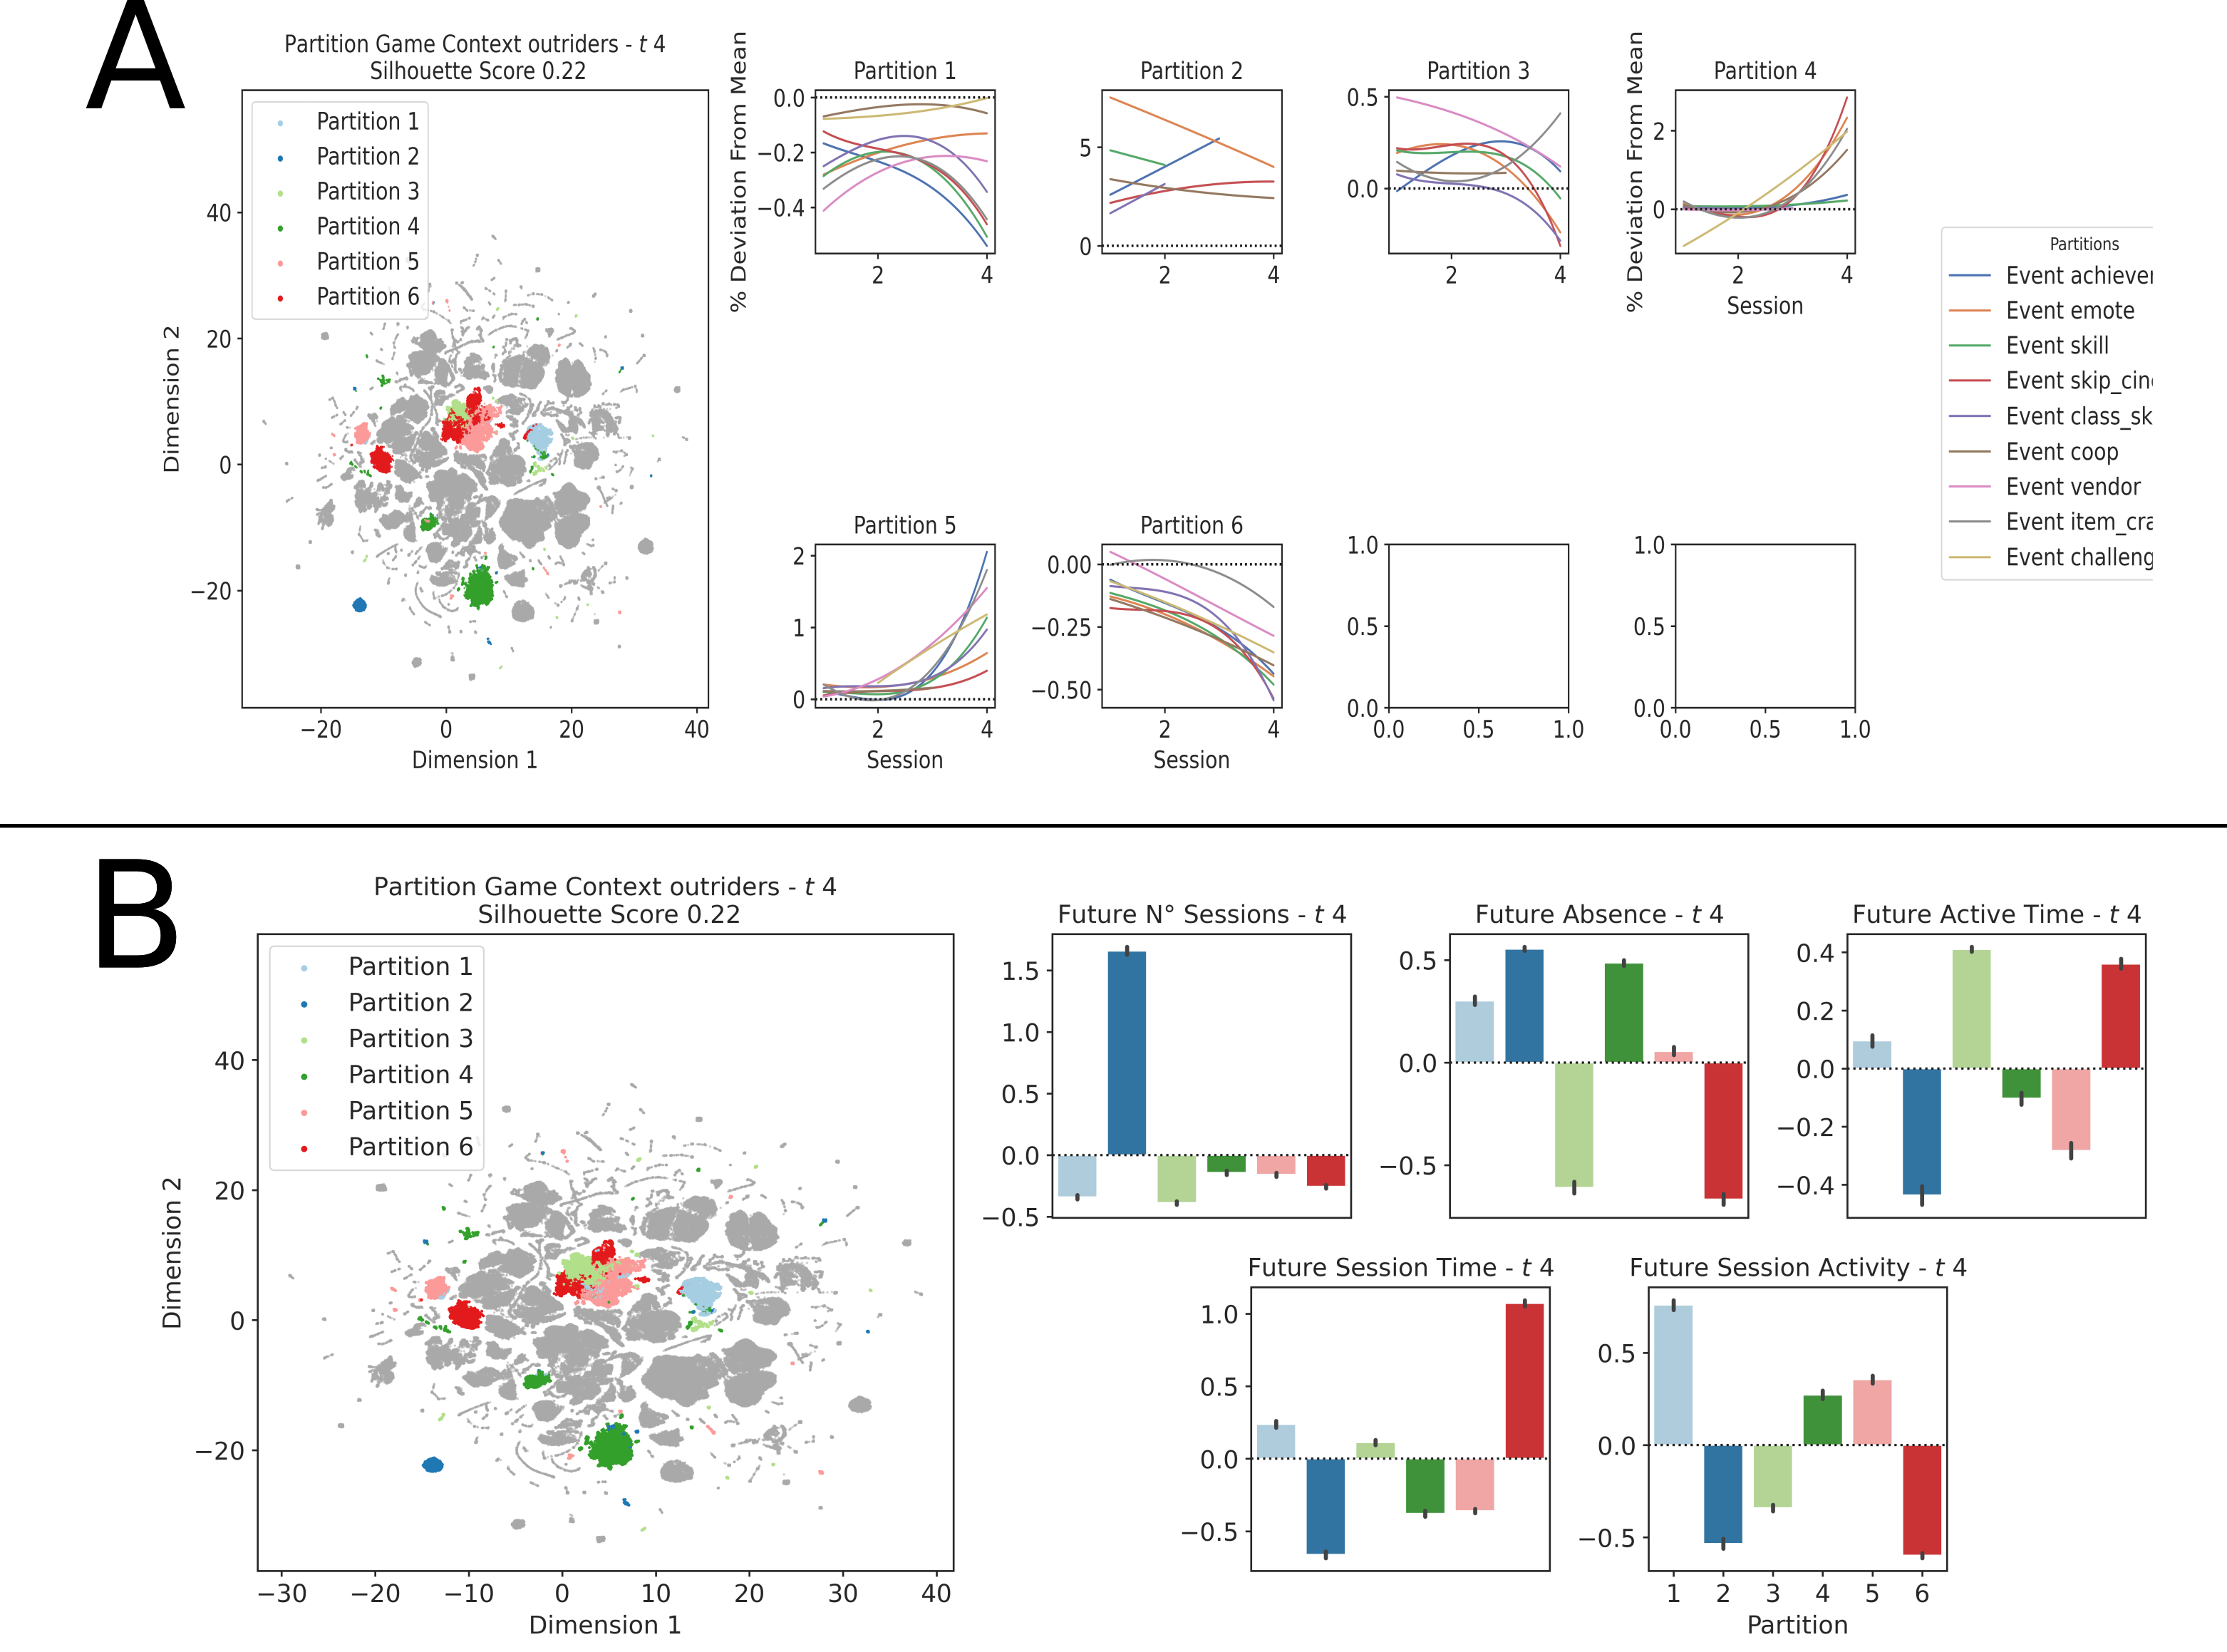
\includegraphics[width=\textwidth]{images/chapter_4/clust_even_outr.png}
\centering
\caption[\textbf{Partitions of the representations generated by the RNN architectures from the game events metrics}]{Panels show the individuated partitions and associated profiles for the representation encapsulating all the game events information up to $t4$. Each panel reports the conventional UMAP reduction of the inferred latent representation with the colours representing membership to a specific partition individuated by the Mini-batch KMeans. Panel A shows for each partition the share of events triggered during each considered game session expressed as number of standard deviations from the sample mean (i.e. z-scores). This information is conveyed through the line of best fit provided by a generalized additive model \cite{serven2018}. Panel C shows, similarly to Figure \ref{partition_rnn_behaviour} , differences in the predictions produced by the model for each partitions. The x axis indicates the partition number while the y axis the expected prediction made for a specific partition. The y axis is expressed in terms of number of standard deviations from the sample mean (i.e. z-scores) with black line indicating the 95\% confidence interval.}
\label{clust_even_outr} 
\end{figure}

\section{Discussion}
As mentioned in section  \ref{incentive_salience}, incentive salience attribution produces latent representations of objects that, when imbued with value, make future interactions with those objects more likely and intense \cite{berridge1998role,berridge2004motivation}. 

The fact that the representation generated by our model could be effectively described by a relatively small number of dimensions (potentially two) appeared to be in line with this and compatible with the idea presented in section \ref{motivation} that motivation-related internal states can be compared to the magnitude of a two-dimensional vector. This metaphor of the "motivational vector" seems to be compatible with the global-local organization of the representation generated by the RNN architecture and its improved version. 

At the global level, different game 'objects' were organized in distinct and coherent regions (see Figure \ref{full_panel_static}A) showing how the model attempted to operate on a meta-level by partitioning a global representation in several object-specific ones. This finding aligns with what highlighted in various work on neural manifold where the responses related to qualitatively different stimuli tends to show a cluster-like organization when reduced to a lower dimensional space \cite{stopfer2003intensity, gallego2017neural, ganmor2015thesaurus}. 

At the local level, each object-specific representation showed an internal gradient-like organization distinguishing individuals based on the estimated intensity of their future interactions with that specific object. This was true for each of the considered behavioural targets (see Figure \ref{full_panel_static}A) showing how the model attempted to provide an holistic description of the intensity of future interactions. The presence of this type of gradient-like organization emerged in work by Nieh et al. \cite{nieh2021geometry} when analyzing neural responses during an evidence accumulation task in virtual reality. When reducing the neural activity to a three-dimensional space, the resulting manifold presented a clear gradient able to code simultaneously for position and levels of accumulated evidence \cite{nieh2021geometry}. A similar finding was present in the work by Stopfner et al. \cite{stopfer2003intensity} where the manifold structure extracted from the activity of olfactory neurons was able to represent qualitative and quantitative differences between odours through a global-local organization similar to that showed in section \ref{functional_properties}.

The dynamic nature of the representation generated by our approach also fits nicely with that of attributed incentive salience \cite{toates1994comparing,robinson1993neural,zhang2009neural,tindell2009dynamic,berridge2012prediction}. In particular, the fact that the aforementioned global-local organization is maintained over time (see Figure \ref{full_panel_temporal}A) corroborate the hypothesis that our model approximated state changes originated from a dynamic process. In support of this, we also observed that the representation generated by our model was spatially coherent over time: it produced distinct regions of low and high expected intensity between which individuals moved over time (see Figure\ref{full_panel_temporal}D). These results appear to match the definition of motivation and incentive salience attribution specified in section \ref{motivation}: a single overarching process able to dynamically predict the likelyhood and intensity by which individuals will interact with a varied set of objects \cite{simpson2016behavioral,toates1994comparing,berridge2004motivation,zhang2009neural}. 

Many other cognitive and affective functions might rely on a latent representation that is functionally similar to the one described in our work (e.g. credit assignment and optimal control \cite{wang2018prefrontal, barto2004reinforcement, friston2012active}, cognitive control, learning \cite{skinner1965science},various forms of reward processing \cite{schultz1997neural, schultz2000reward}). Similar to attributed incentive salience, these functions are all involved in generating motivated behaviour and heavily rely on reward signals, however none of them is concerned with attributing and describing the motivational saliency that an object possess. This is made evident in the works by McClure et al. \cite{mcclure2003computational} and Zhang et al. \cite{zhang2009neural} where the system involved in salience attribution is functionally separate from the one assigning credit and executing actions: the former provide a representation that informs and biases the decisions taken by the latter serving an almost exclusively qualifying role (see the role of attributed incentive salience in addiction-like conditions \cite{robinson1993neural}). Similarly, the representation generated by our model does not provide any insight on the decision making process underlying the observed playing behaviour but simply provide an approximate description of the "motivational pull" that a particular game object has on a particular individual at a certain point in time. 

The functions encoded by the hidden units constituting the representation appeared to have a series of distinctive properties, namely: redundancy, non linearity, multiplicity (single units code for multiple functions) and consistency over time. These may have played a role in providing the representation generated by our model with its distinctive characteristics. For example, as we mentioned in section \ref{manifold_rep_incentive_salience} redundancy and inter-correlation are characteristics of the signals from which the manifold representation of internal states arises \cite{seung2000manifold,gallego2017neural}. Multiplicity on the other hand, might be the factor underlying the ability of our model to produce a single unitary representation which holds predictive power over different behavioural targets. Finally, consistency over time could be the mechanisms supporting the type of temporal coherence observed in panel \ref{full_panel_temporal}D. We want to stress that these findings are to be considered exploratory in nature since they do not rely on \textit{a-priori} hypotheses. A comparison between these computational properties and those underlying the attribution of incentive salience is required and would constitute a potential venue for future investigations. 

The introduction of environmental and game event covariates appeared to have produced a more consistent representation (see Figures \ref{rnn_env_even_full_shared} \ref{rnn_predictive_comparison}) with better discriminatory powers, a finding in line with the, although marginal, improvements in predictive performance observed in section \ref{results_3}. It might be speculated that this improvement was associated both with the introduction of new informative covariates and with the ability of the architecture to separately model their contribution. Indeed, similarly to the idea underlying Neural GAMs \cite{agarwal2021neural}, different portion of the architecture might have focused on inferring specialized functions then combined in a more effective latent representation.

However, the major advantage provided by separately modelling the contribution of behavioural, environmental and game-events metrics lied in the ability to obtain distinct representations that we were able to leverage for exploratory analyses. This allowed us to perform time series partitioning at a much larger scale that has been previously done in the videogames literature (potentially up to millions of time series) \cite{bauckhage2014clustering, makarovych2018like, vihanga2019weekly, aung2019trails}. Indeed, previous approaches in the literature attempted to cluster or partition directly the observable data space, a particularly cumbersome process for univariate and multivariate time series, especially if suitable techniques like Dynamic Time Warping \cite{muller2007dynamic} are to be used. In our case by leveraging the representational power of ANNs we were able to condense the information present in the the time series data to a more compact representation, this allowed us to then rely on relatively inexpensive algorithm (i.e. Minini-Batch KMeans) for performing the partitioning.

The partition analysis conducted on the behavioural representation allowed to individuate a set of profiles that are, to a certain extent, consistent with behavioural correlates of different levels of attributed incentive salience \cite{berridge2004motivation} and general operant conditioning principles \cite{thorndike1927law, skinner1953science, nevin2000behavioral}: the strength of past interactions positively correlate with the frequency and intensity of future ones. The various offsets that each partition showed might suggest different levels of predisposition towards the various game-objects. The dynamic nature of these profiles provided a more granular characterization allowing to observe variations in the entire history of interactions and not just in the expected intensity of future ones. For example, it was possible to see how a higher likelihood of future interactions was supported both by a history of low intensity but high frequency interactions as well as by a series of high frequency and high intensity interactions. In this sense, these behavioural profiles can be seen as useful devices for investigating the existence of inter-individual differences in schedules of interactions with potentially rewarding objects. 

On the other hand, partitioning the environmental representation provided us with insights on how different individuals distributed their interactions with a videogame over days of the week and hours of the day. We were able to replicate some of the findings of Vihanga and colleagues \cite{vihanga2019weekly, wannigamage2021player}, identifying similar profiles of interactions. However, our approach allowed us to gather insights not just on the characteristics of the different profiles but also on their potential impact on interaction intensity. A similar conclusion can be drawn from the partitioning of the game events representation. We were able to identify not just  how different groups of individual distributed their playing activity between different in-game events but also how these evolved over time. Moreover in contrast to the work of Makarovych et al. \cite{makarovych2018like}, our approach did not just identify frequent patterns of interactions with in-games elements but also the associated variations in the intensity of future behaviour.

\chapter{Model Application and Pipeline}
\label{chapter_appliction}
\section{Introduction}
\label{industry_needs}
As we mentioned in chapter \ref{chapter_general_intro}, despite the main aim of this thesis has been to derive a methodology for approximating the motivational state of individuals while interacting with potentially rewarding object (a videogame in this case), a secondary objective was to illustrate the potential application of this methodology within an industrial setting.

In this view, this chapter will focus on sketching the design of a system relying on our methodology for automated engagement prediction. First we will introduce a set of ethical considerations that should be taken into account when designing such system. Subsequently, we will provide an overview on why an industry player (or groups thereof) might need a process for quantifying and predicting engagement and which characteristics this process should have. Finally we will proceed at illustrating a system designed for serving this need, placing particular emphasis on how its components connect with the work presented so far.

\section{Some Ethical Consideration}
\label{ehtical_considerations}
Automated system leveraging behavioural data are now-days used extensively in both low and high stakes scenarios \cite{mehrabi2021survey}, with the potential to have a direct and concrete impact on individuals. For this reason, when designing automated data-driven applications, issues related to fairness should be taken into account. 

By fairness we entail the set of principles and considerations that in recent years are adopted in order to avoid that decisions based on a machine-learned model do not inadvertently bring harm to specific groups of people \cite{mehrabi2021survey}. A complete overview of the issue of fairness in machine learning would be beyond the scope of not just this section but the entire thesis, as it is a vast landscape \cite{mehrabi2021survey} hard to navigate due to its many levels of complexity \cite{corbett2018measure}.  We will therefore focus on three major aspects related to the work presented in this chapter. 

The first aspect concerns biases present in the data on which a machine learning algorithm is fitted. These might be induced by an over or under representation of certain strata of the population that an automated system will ultimately need to serve \cite{mehrabi2021survey}. Given how a large part of machine learning algorithms are fitted to the data (e.g., maximum likelyhood) the risk is that the prediction produced by the algorithm will revert to the mean or in the worst case, will result to be biased with respect to the true characteristics of the population \cite{corbett2018measure, mehrabi2021survey}. Despite the harm that these biases might cause in the context of engagement prediction is not as pronounced as in other areas (e.g., credit, criminal or medical risk assessment), they can still have unexpected repercussion on an individual if they assume that people engage in similar ways regardless of situational, personal and cultural differences. For example an individual might receive notifications in inappropriate contexts (e.g.,  during an emotionally challenging period) or be unfairly penalized within the game world (e.g., due to irregular playing patterns caused by personal or situational reasons) because they deviate from what is the expected behaviour in the data on which the algorithm was fitted.

To this connects the second aspect of fairness that we want to highlight, namely the risk of inadvertently cause harm to individuals which are either temporarily or structurally subject to some form of vulnerability. This might happen as a consequence of automated decision making based on what we call "unconstrained model predictions", what we mean by this is when the predictions from a model are used verbatim without knowing the context in which they will be applied. For example, if we imagine a system aimed at individuating high spending users within a game relying on gacha or loot-box mechanics, relying on unconstrained predictions might in this case inadvertently target individuals with a predisposition to or an history of problematic gambling behaviour \cite{petrovskaya2022prevalence}. The most problematic aspect related of this issue is that often the information required for "constraining" an "unconstrained prediction" are not available to the system, either because they are not easy to derive (e.g., they are not directly observable) or should not be accessible (e.g., they are Personal Identifiable Information - PII \cite{EUdataregulations2018}).

Related to the first two points is the third and final aspect of fairness that we would like to address which is connected with the right to object specified by the General Data Protection and Regulation act (GDPR) \cite{EUdataregulations2018} which allows an individual to object to the processing of their data in any form and at any moment. Despite this aspect is partially attenuated by rights granted by the GDPR (although this interests exclusively the European Union), it only covers the processing of data rather than the effect connected with automated decision making. An individual might object to the inclusion of their data during the decision making process but still be subject to the effect of this last one, for example if the system entails a policy of blanket intervention based on the average user behaviour for all those individuals for which no data are available.

As we mentioned at the beginning of the paragraph, an exhaustive treatment of these issues and the relative mitigating actions that could be taken is beyond the scope of the current work. Nevertheless we want to stress that addressing them in an effective manner is of pivotal importance when automated systems based on machine-learning (or other form of statistical decision making) becomes part of the operations of an industry player.

\section{Autometed Engagement Quantification and Prediction in a Videogame Setting}
\label{industry_needs}
As we mentioned before, in an industry setting the development of research projects often aims at the the resolution of specific problems or at the improvement processes central to its success (being it measure in terms of revenues or perceived quality of goods and services). 

So where does engagement quantification and prediction sits within the needs of the videogame industry? Very often (if not always) the success of a videogame title is strictly connected with either its ability to retain users or with the experience that users had with the product (i.e., a videogame title) \cite{amit2001value, alomari2016mobile}. The first is pivotal in scenarios where games are treated as a service sold to an audience (similarly to the function of streaming services) while the second is more relevant in situations where games are considered digital goods \cite{amit2001value, alomari2016mobile}. 

In this context, engagement can be viewed as a measure of how a particular game was, is or will be able to retain users. For example, if an individual is engaged with a particular service (e.g., a videogame) it is likely that will keep paying a subscription (or any other form of pay-to-consume) for said service. Similarly, if an individual had a good experience with a particular digital good, it is is more likely that will promote it to other potential users, acquire similar products or buy products from the same seller.  

In this view being able to estimate the propensity that a user (or a group of users) has towards a particular game translates (in a more or less direct way) to the capacity of assessing if a game is likely to be a success of public and revenue. For this reason it is often the case that videogame publishers and studios try to leverage the information they have available through telemetry system for taking the stock of how a particular game is performing \cite{el2016game}. 

This is the classical example of analytical reports summarizing various type of Key Performance Indicators \cite{el2016game} or profiling techniques describing how users interacted with a particular game \cite{el2016game}. Despite this approaches are extremely relevant for gathering insights on the perfromance of a particular game title, they only allow to execute what we call "reactive" interventions. By reactive interventions we mean that mitigating actions for improving a sub-optimal situation (e.g., when a videogame is unable to foster engagement) can only be taken \textit{ex-post}.

On the other hand, interventions based on the outcomes of a predictive model are by definition "pro-active". This because by knowing in advance if a particular situation is going to be problematic or not allows to plan and deliver mitigating actions \textit{ex-ante} \cite{el2016game, el2021game}. It is worth noticing that approach based on the outcome of predictive models are not incompatible with techniques used within a "reactive" framework (e.g., reports and profiles) but rather complementary. For example the same KPI calculated on observed data can and should be computed also on predictions and forecast generated by a machine-learned model. Similarly, it is possible to create profiles that not just describe the historical interactions of users with a particular game but that are also informative of the expected future engagement of such users.

Within this last "pro-active" framework lies the work that we presented in this thesis. We will now proceed at illustrating the design of a system aimed at delivering predictions and insights that can to foster \textit{ex-ante} interventions for the mitigation and improvement of videogames engagement.

\section{System Design Diagram}
\label{pipeline}


\begin{figure}[ht]
\centering
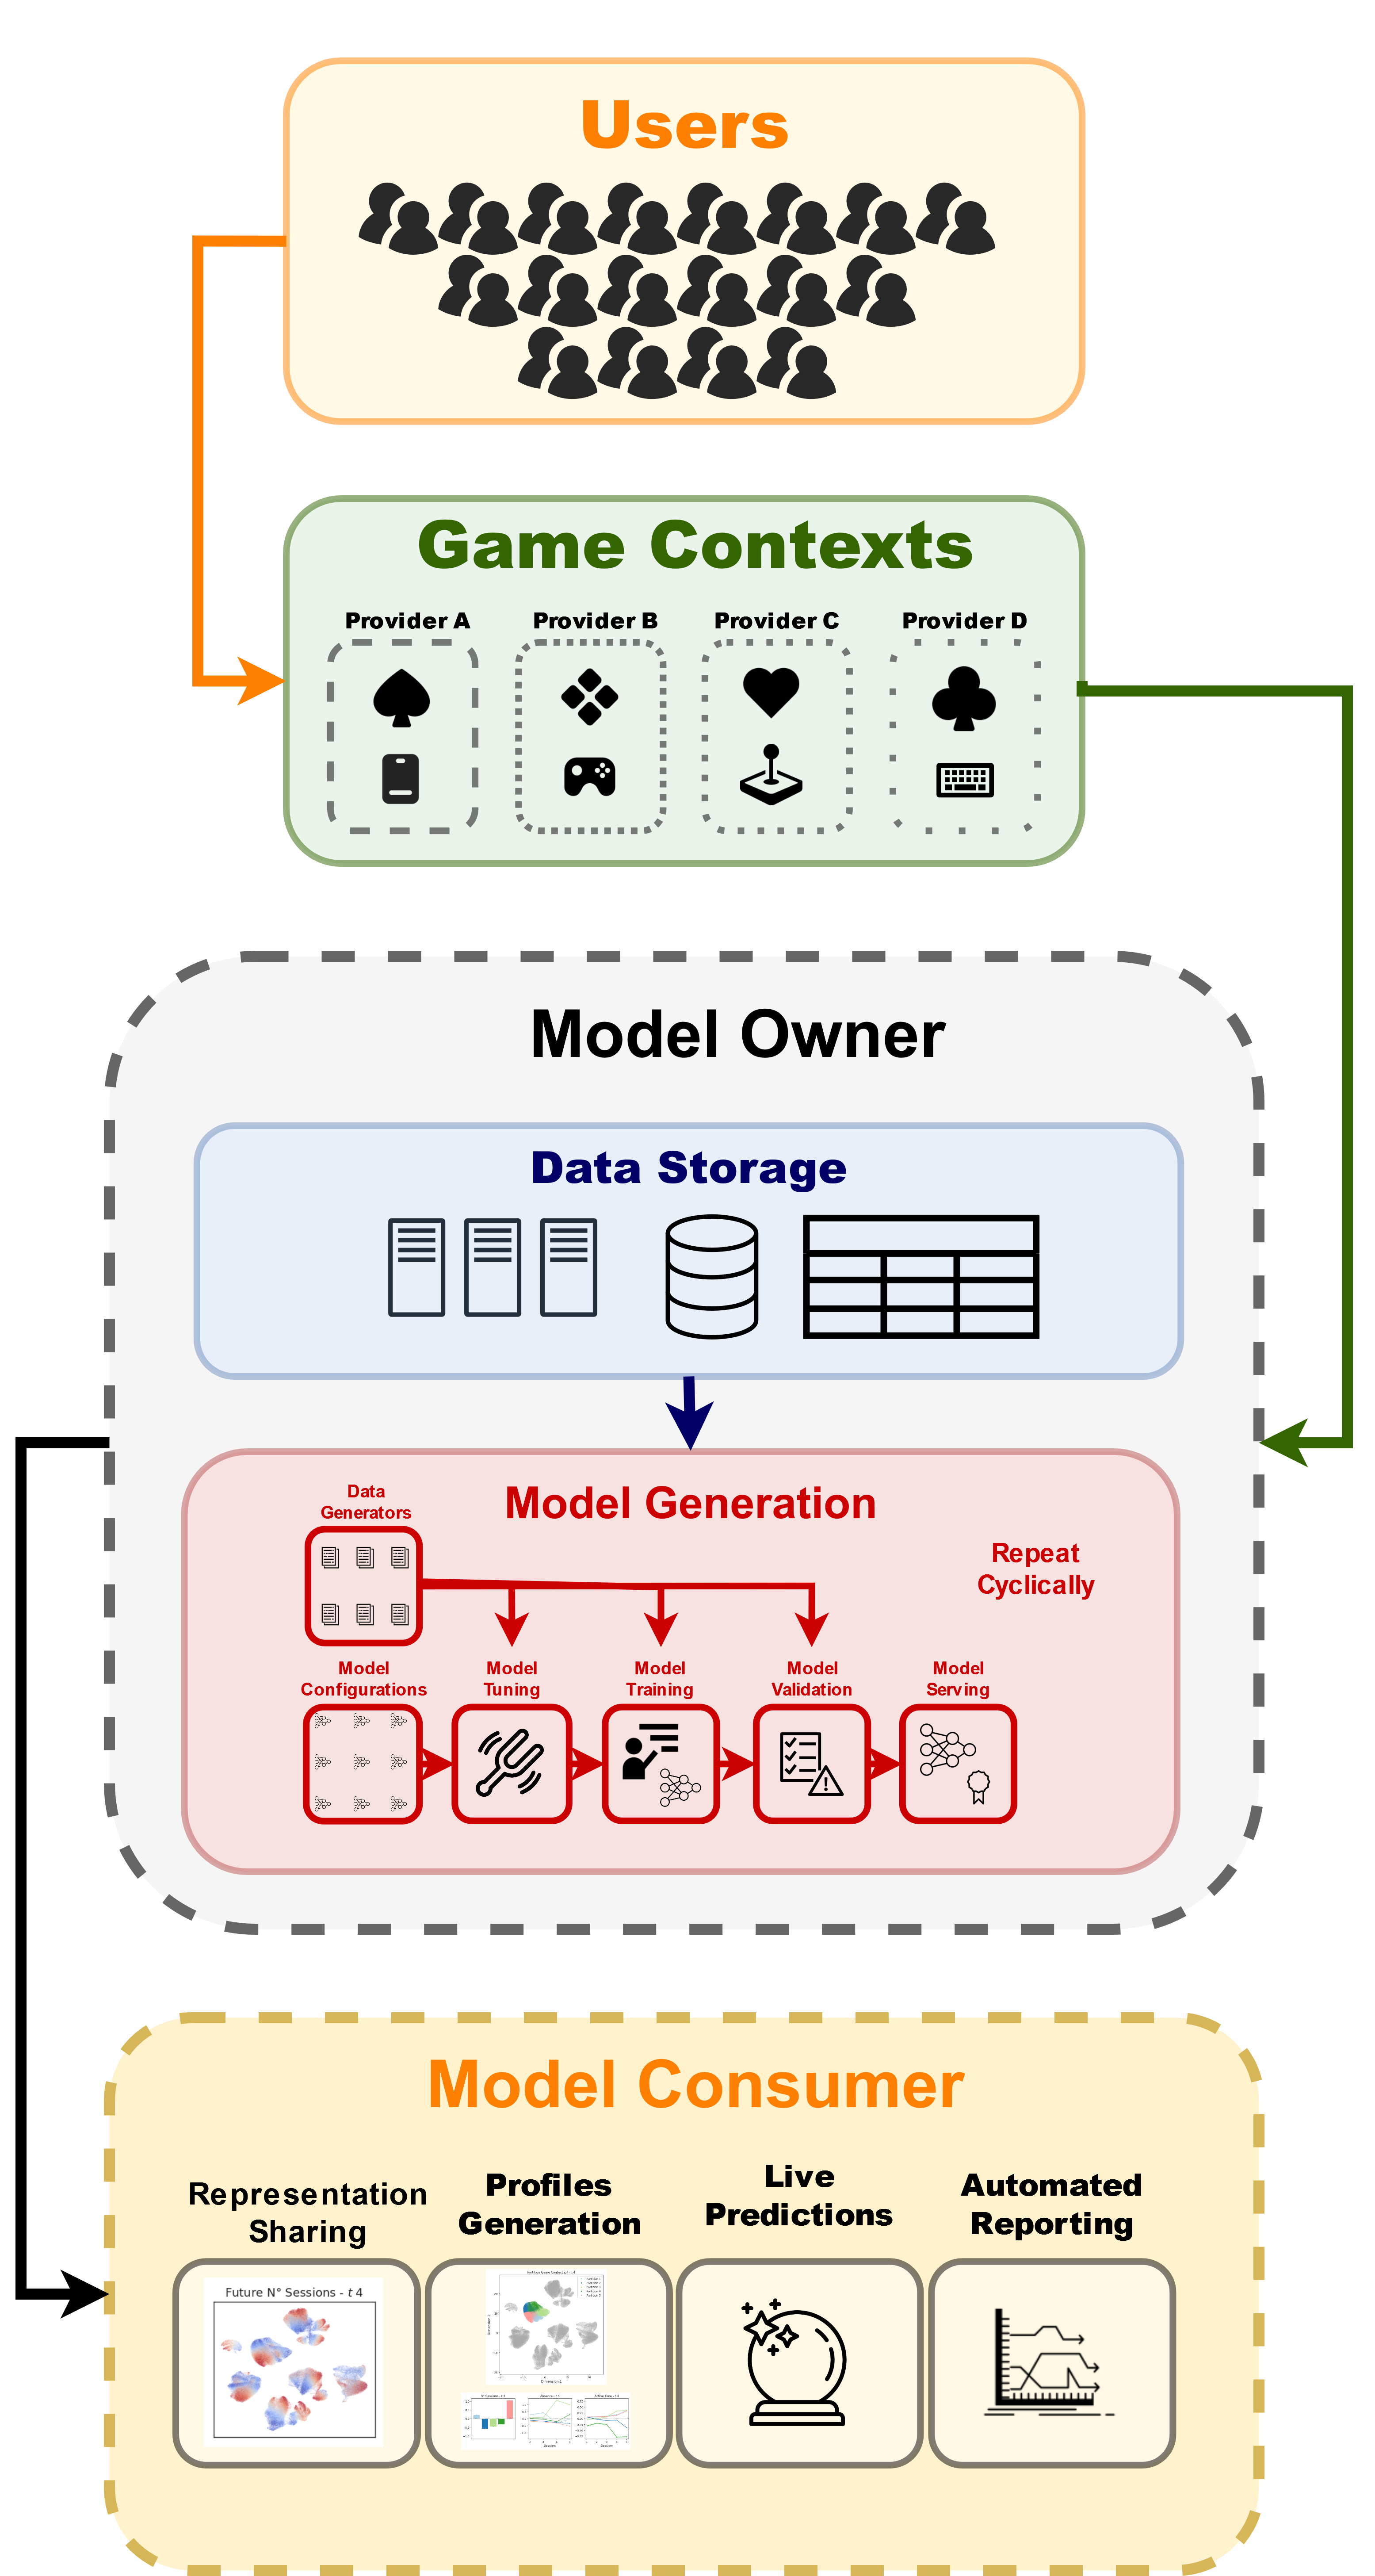
\includegraphics[width=0.7\textwidth]{images/chapter_5/pipeline_diagram.png}
\caption[\textbf{Model Deployment Pipeline}]{The figure represents a simplified system diagram for a potential application of the improved RNN architecture. Solid lines represent low-level components in the system while dashed lines indicate high-level entities. Directional arrows represent the flow of operations inside the system.}
\label{pipeline}
\end{figure}

\section{Data Generation}
\label{data_generation}
This is the first component of the system and describes the entities generating the data that will then be used by the system. It is composed by two major elements: the users and the game contexts. 

The relationship between these two entities has already been described in chapter \ref{chapter_lit_review} and chapter \ref{chapter_theory_modelling} in particular. In line with the framework that we adopted through out this thesis we assume that each game context posses properties (defined by their structural characteristics) that might result more or less rewarding to different users. By means of repeated interactions with the game contexts the users learn about these properties and progressively updates latent representations of the various contexts. These representations, which as we said in chapters \ref{chapter_lit_review} and \ref{chapter_theory_modelling} are imbued with value, act by either promoting or demoting future engagement with the game contexts quantifiable by means of metrics of behavioural frequency and intensity.

The various game contexts can be managed by a single or multiple entities and are usually provided through different type of systems. For example, the game contexts utilized for this thesis were managed by a single entity (i.e., our partner company Square Enix Ltd.) and provided through an array of different hardware systems: smartphones, personal computers and gaming consoles. Ultimately, the software and console hardware make up the game context with which the users interact and within those lies the telemetry system in charge of recording the behavioural metrics and transmitting them to the relevant data storage system.

\section{Model Owner}
\label{model_owner}
This component represents the entity responsible for the acquisition ad storage of data generated by the interactions between the users and the game contexts. It is also in charge of managing all the operations necessary for fitting a learning algorithm to the data and validating the derived model. 

It is relevant to highlight that the model owner usually corresponds one-to-one with the entity managing the game contexts but the two don't necessarily  have to coincide. In the context of federated learning  \cite{yang2019federated} for instance, a model owner might distribute copies of the learning algorithm across separate entities and only act as a pooling mechanism  once they have been fitted to the data \cite{kairouz2021advances}. In this case, the entities don't necessarily need to be known to the model owner or to each other, in fact this information must be kept hidden. Indeed, the aim of federated learning is to generate global and robust model fitted on multi-source data while being compliant with strict privacy constrains \cite{yang2019federated, kairouz2021advances}. 

That said, for simplicity in this section we will focus on a situation where the model owner is one with the entity managing the game contexts.

\subsection{Data Storage}
Once the in-game behaviour resulting from the interaction between the users and the game contexts have been recorded by the telemetry system

\subsection{Model Generation}
\lorem
\paragraph*{Data Generators} \lorem
\paragraph*{Model Configurations} \lorem
\paragraph*{Model Tuning} \lorem
\paragraph*{Model Training} \lorem
\paragraph*{Model Validation} \lorem
\paragraph*{Model Serving} \lorem

\section{Model Consumer}
The model consumer identifies the entity interacting with the model and leveraging its outputs. As specified in section \ref{model_owner} this doesn't necessarily have to correspond to the model owner but it is supposed to be identified in at least one of the entities managing the game contexts. Again, for simplicity we will assume that in this case they all corresponds to the same entity. The model consumer shouldn't have direct access to the algorithm generated by the model owner nor should be able to alter its inner working (e.g., it should be able to re-fit the algorithm on a new set of the data), its only focus should be to consume its output for different type of applications. We will now proceed at briefly illustrating some of these applications.

\subsection{Representation Sharing}
\lorem
\subsection{Profile Generation}
\lorem
\subsection{Live Predictions}
\lorem
\subsection{Automated Reporting}
\lorem


\chapter{General Discussion}
\label{chapter_general_discussion}
The present work outlined a method for embedding theory-driven knowledge in data-driven approaches, allowing to more easily interpret and test hypotheses on the representation they produce. In comparison to other works focusing on the identification of latent states (or their manifold representation) from behavioural data \cite{calhoun2019unsupervised, luxem2020identifying, pereira2020quantifying, shi2021learning, mccullough2021unsupervised}, the present methodology offers a series of advantages. It does not require the Markov assumption, it generates continuous rather than discrete state space (hence the number of hidden states doesn't need to be specified) and it relies on a more easily scalable class of algorithms. Moreover, in contrast with a general tendency of utilising completely unsupervised techniques for capturing the manifold structure underlying behavioural data \cite{calhoun2019unsupervised, luxem2020identifying, pereira2020quantifying, shi2021learning, mccullough2021unsupervised}, our methodology attempts to extract representations which obey to specific functional constrains (see section \ref{manifold_learning}) and can therefore be more easily interpreted within a specific theoretical framework. Our approach offers a convenient framework for dealing with a diverse series of tasks. It allows to produce predictions of the amount and intensity of future interactions that an individual will have with a specific object. It generates a representation that can be analyzed (similarly to what has been done in section \ref{representation_analysis}) or provided as input to other algorithms. Indeed, the encoder mentioned in section \ref{representation_analysis} can be thought of as an automatic feature extractor. This can be used to reduce complex time series data of varying length to fixed-size vectors able to describe the propensity of an individual to interact with an object. For example, the analysis presented in section \ref{partition_analysis} showed how this process could be applied for time-series partitioning of large dataset. The present work leveraged data coming from video games but the adopted approach could easily be applied to other contexts. They only key requirement is the access to behavioural quantifiers describing the amount and intensity of interactions that an individual has with a particular object, service or task. This means that natural areas of application for our approach are those relying on the remote acquisition of behavioural data (e.g. web services or online experiments) but also situations in which large volumes of experimental data are available (e.g. large multi-center studies).  

\section{Limitations and Future Directions}
The work we just presented is not exempt from limitations. First, since our approach is attempting to solve an inverse problem, the issue of uniqueness arises. Many different latent states might have produced the behavioural patterns that our model observed and there is no guarantee of a strict one-to-one mapping between the representation generated by our model and attributed incentive salience.  As we mentioned in section \ref{videogame_telemetries} the reward dynamics generated by the interaction between the individual and the game incentive mechanics play an important role in determining the intensity of future playing behaviour \cite{agarwal2017quitting, avserivskis2017computational, wang2018beyond}. In addition to this, we know that these dynamics are modulated by the internal state of the individual \cite{zhang2009neural} and by the context in which in which they are generated \cite{palminteri2015contextual}. These factors, were only partially captured by our approach as they require a higher temporal resolution (i.e. within rather than between sessions) as well as more granular indices (i.e. in-game and environmental information) than those we employed. As a consequence we can see how our approach, despite outperforming competing ones, still achieves a relatively high error rate in predicting some behavioural targets (e.g. future Absence). The behavioural profiles individuated by the partition analysis generally reflect those predicted by theories of reward-driven motivation \cite{thorndike1927law,skinner1965science,berridge2004motivation} but they also show some unexpected and potentially contradictory results (see the differences between partitions 1 and 2 and between partitions 3 and 4 in Figure \ref{partitioning}B). Given the observational setting and the unsupervised learning analysis we adopted, the explanations provided in section \ref{partition_analysis} should be taken with caution and be seen mostly as a starting point for future investigations. Clarifying the the nature of these discrepancies may require experimental work in more controlled settings. Lastly, despite the fact that our approach appeared to deal gracefully  with objects having different structural characteristics, these were limited to the domain of video games. In order to verify the generalizability of our approach, future work should include data generated from a variety of contexts (e.g. web services, online and laboratory-based experiments).

\bibliographystyle{unsrt}
\bibliography{bibliography}

\end{document}

%%%%%%%%%%%%%%%%%%%%%%%%%%%%%%%%%%%%%%%%%%%%%%%%%%%%%%%%%